\documentclass[12pt,
	a4paper,
	listof=totoc,
	bibliography=totoc,
	parskip=full*
	]{scrreprt}

\usepackage[utf8]{inputenc}
\usepackage[ngerman]{babel}
\usepackage[babel,german=quotes]{csquotes}
\usepackage[hidelinks]{hyperref}
\usepackage{amsmath}
\usepackage{paralist}
\usepackage{amsfonts}
\usepackage{amssymb}
\usepackage{caption}
\usepackage{pdfpages}
\usepackage{graphicx}
\usepackage{tabularx}
\usepackage{tabu}
\usepackage{enumerate}
\usepackage{enumitem}
\usepackage{adjustbox}
\usepackage[toc,page]{appendix}
\usepackage{subfigure}
\usepackage[left=3.00cm, right=2.00cm, top=1cm, bottom=1.5cm,includeheadfoot]{geometry}
\usepackage{scrpage2}
\pagestyle{scrheadings}
\usepackage{todonotes}
\usepackage{fixltx2e}
\usepackage[toc,nonumberlist,acronym,style=super]{glossaries}
\usepackage{float}
\usepackage{wrapfig}
\usepackage{lscape}
\usepackage{rotating}
\usepackage{blindtext}
\usepackage{booktabs}
\usepackage[backend=bibtex,style=ieee,sorting=nty]{biblatex}
\usepackage{listings}
\usepackage{color}
\usepackage{courier}
\usepackage{tablefootnote}
\usepackage{slashbox}
\usepackage{multirow}
\usepackage{mathtools}
\usepackage{blindtext}

\renewcaptionname{ngerman}{\bibname}{References}
\renewcommand\appendixtocname{Appendix}
\renewcommand\appendixpagename{Appendix}
\setcounter{secnumdepth}{3}

\newcommand{\mytitle}{Building Conversational Dialog-Systems using Sequence-To-Sequence Learning}
\newcommand{\myauthor}{Dirk von Grünigen, Martin Weilenmann}

\newcommand{\ra}[1]{\renewcommand{\arraystretch}{#1}}
\newcommand{\quotes}[1]{``#1''}
\newcommand{\fixme}[1]{\todo[linecolor=red,backgroundcolor=red!25,bordercolor=red]{#1}}
\newcolumntype{M}{>{\begin{varwidth}{4cm}}l<{\end{varwidth}}} %M is for Maximal column

\definecolor{dkgreen}{rgb}{0,0.6,0}
\definecolor{gray}{rgb}{0.5,0.5,0.5}
\definecolor{mauve}{rgb}{0.58,0,0.82}

\lstset{frame=tb,
  language=python,
  aboveskip=3mm,
  belowskip=3mm,
  showstringspaces=false,
  columns=flexible,
  basicstyle={\small\ttfamily},
  numbers=none,
  numberstyle=\tiny\color{gray},
  keywordstyle=\color{blue},
  commentstyle=\color{dkgreen},
  stringstyle=\color{mauve},
  breaklines=true,
  breakatwhitespace=true,
  tabsize=3
}

\newcommand{\specialcell}[2][c]{%
	\begin{tabular}[#1]{@{}c@{}}#2\end{tabular}}

\bibliography{biblio}
\nocite{*}

% Glossar entries

\newglossaryentry{cell}
{
	name={Cell},
	description={Any instance of any kind of RNN layer is called a cell}
}

\newglossaryentry{corpus}
{
	name={Corpus},
	description={Refers to the raw data used to build the datasets}
}

\newglossaryentry{dataset}
{
	name={Dataset},
	description={Refers to the dataset resulting from the preprocessing of the raw corpus}
}

\newglossaryentry{epoch}
{
  name={Epoch},
  description={One iteration through all of the training data is called an epoch}
}

\newglossaryentry{encoder}
{
	name={Encoder},
	description={Part of seq2seq models responsible for processing the input sequence}
}

\newglossaryentry{decoder}
{
	name={Decoder},
	description={Part of seq2seq models responsible for generating the output sequence}
}

\newglossaryentry{neuron}
{
  name={Neuron},
  description={Basic building blocks of NN. Models a mathematical function}
}

\newglossaryentry{layer}
{
  name={Layer},
  description={Collection of multiple neurons. An NN usually consists of several of these layers}
}

% Acronyms
\newacronym{CPU}{CPU}{Central Processing Unit}
\newacronym{GPU}{GPU}{Graphical Processing Unit}
\newacronym{NN}{NN}{Neural Network}
\newacronym{RNN}{RNN}{Recurrent Neural Network}
\newacronym{LSTM}{LSTM}{Long Short-Term Memory Network}
\newacronym{Seq2Seq}{Seq2Seq}{Sequence-To-Sequence}


\makeglossaries

\title{\mytitle}
\author{\myauthor}

\begin{document}

\begin{titlepage}
	
	\newcommand{\HRule}{\rule{\linewidth}{0.5mm}} % Defines a new command for the horizontal lines, change thickness here
	
	\center % Center everything on the page
	
	%----------------------------------------------------------------------------------------
	%	HEADING SECTIONS
	%----------------------------------------------------------------------------------------
	
	\textsc{\LARGE ZHAW}\\ % Name of your university/college
	\textsc{\Large Zurich University of\\Applied Sciences}\\[1.0cm]
	\textsc{\Large Bachelor-Thesis}\\[0.5cm] % Major heading such as course name
	\textsc{\large FS 2017}\\[0.5cm] % Minor heading such as course title
	
	%----------------------------------------------------------------------------------------
	%	TITLE SECTION
	%----------------------------------------------------------------------------------------
	
	\HRule \\[0.4cm]
	{ \LARGE \bfseries \mytitle}\\[0.4cm] % Title of your document
	\HRule \\[1.5cm]
	
	%----------------------------------------------------------------------------------------
	%	AUTHOR SECTION
	%----------------------------------------------------------------------------------------
	
	\begin{minipage}{0.4\textwidth}
		\begin{flushleft} \large
			\emph{Authors:}\\
			Dirk \textsc{von Grünigen}\\
			Martin \textsc{Weilenmann}
		\end{flushleft}
	\end{minipage}
	~
	\begin{minipage}{0.4\textwidth}
		\begin{flushright} \large
			\emph{Supervisors:} \\
			Dr. Mark \textsc{Cieliebak}\\
			Dr. Stephan \textsc{Neuhaus}
		\end{flushright}
	\end{minipage}\\[2cm]
	
	% If you don't want a supervisor, uncomment the two lines below and remove the section above
	%\Large \emph{Author:}\\
	%John \textsc{Smith}\\[3cm] % Your name
	
	%----------------------------------------------------------------------------------------
	%	DATE SECTION
	%----------------------------------------------------------------------------------------
	
	{\large \today}\\[2cm] % Date, change the \today to a set date if you want to be precise
	
	%----------------------------------------------------------------------------------------
	%	LOGO SECTION
	%----------------------------------------------------------------------------------------
	
	
\includegraphics{img/logo_zhaw}\\[1cm] % Include a department/university logo - this will require the graphicx package
	
	%----------------------------------------------------------------------------------------
	
	\vfill % Fill the rest of the page with whitespace
	
\end{titlepage}

\includepdf{img/declaration_of_originality}

% \newgeometry{top=0.75cm,bottom=1cm}
\chapter*{Abstract}
Das Ziel dieser Arbeit war ein Nachbau des Dialogsystems aus dem Paper \cite{}, inspiriert durch Beispiele maschineller Antworten wie: Human: "what is the purpose of being intelligent?" Machine: "to find out what it is .". Die Bedingungen für den Nachbaue waren ein wenig erschwert, da wir nu auf einer GPU die Berechnungen durchführten.

Während dem Nachbau mussten wir einige technische Herausforderungen meistern, bis wir dann endlich ein funktionsfähiges Modell hatten. Die Modelle wurden schlussendlich mit Tensorflow und Seq2seq2 umgesetzt. Wir trainierten anschliessen über 3 Wochen lang zwei Modelle mit unterschiedlichen Trainingsdate. Ein Modell trainierten wir mit OpenSubtitles welche gesprochene Sprache beinhaltet und Eines mit Reddit welcher geschriebener Sprache enthält. 

Anschliesssend untersuchten wir zuerst "quantitativ"? (oder so hast du das genannt) die Entwicklung der Modelle. Während die Trainings und Validierungsmetriken mit fortlaufendem Training besser wurden, wurden diejenigen der Testdaten eher schlechter, oder blieben gleich. Die ernüchternden Resultate waren insofern eine überraschung, da wir beim interagieren durchaus eine Verbesserung verspürten. Aufgrund dieses missmatch untersuchten wir die Vielfalt der Sprache. Diese Ergebnisse deckten sich mit unserem Subjektiven Empfinden.

Am Ende der Arbeit vergleichen wir Anhand einiger ausgesuchter Beispiele unsere replies mit denjenigen von Cleverbot. Zusätzlich entnahmen wir Dialoge aus dem paper \cites{} und verglichen diese mit unseren. Dabei kann unser Modell durchaus mithalten, hätte aber vermutlich in einem breit angelegten Test wenig Chance. Vor allem bei komplexeren Aussagen, scheint unser Modell schwierigkeiten zu haben. Als Ursache vermuten wir einerseits die Grösse des Modells und die Dauer des Trainings. Insgesamt sehen wir den Nachbau aber als Erfolg Aussagen wie: Human: "What are you?" Machine: "i m a bot .",(komma hier, keine ahnug) waren doch überraschend.

In the following thesis we are going to investigate into building a end-to-end conversational dialog system based on a sequence-to-sequence learning and recurrent neural networks. We use an already built system as the reference architecture. The main topic of the research is to investigate if it is possible to use model, which can be trained on a single GPU, and still exhibit similar performance as much larger models.

The first part is dedicated

The analysis of the resulting models is done under several aspects. First, we are going to look into the learning process and try to distinguish differences between using two different datasets for the training. It is shown that the structure and linguistic nature of different datasets has a clear impact on the learning process of such models. Evaluations to asses the performance follow afterwards, which includes tests with a newly proposed metric based on the Sent2Vec library.

The previous analysis reveals several problems our models exhibit. One of the biggest is that such models tend to generate generic responses which leads to deteriorating results. To find an explanation for this behavior we are going to investigate into the way these models We then go on and analyze the problem of generic responses. This analysis shows that 

\tableofcontents
\restoregeometry

\chapter*{Preface}
First and foremost, we want to thank our supervisors Dr. Mark Cieliebak, Dr. Stephan Neuhaus and Jan Deriu for their ongoing support and guidance during the time we were writing this exploratory thesis. The weekly discussions were always a pleasure and helped us a lot to shape our ideas and goals. We also want to express gratitude to our families, colleagues and friends for their patience, support and encouragement to go on, as it was sometimes hard to keep up the motivation, especially in times were everything seemed to go wrong. Last but not least, we also want to thank the Institut für Angewandte Informationstechnologie from the ZHAW for providing us with the computational resources required to conduct the experiments.

\chapter{Introduction}
\blindtext
\chapter{Related Work}
\label{related_work}

The history of dialog systems and chatbots dates further back than most people would probably expect, as the first known dialog system, called \emph{ELIZA}, was already published in the year 1966 by Joseph Weizenbaum~\cite{Weizenbaum:1966}. Even though this system was pretty primitive from a todays standpoint - it used scripted responses instead of learning to talk - it was widely recognized and was considered one of the first contenders to pass the Turing test. One of its successors was then PARRY, which was a chatbot simulating a patient with paranoid schizophrenia~\cite{Colby:1974}. An interesting note here is that it was the first actual computer program to almost pass a special variant of the Turing test as only 48\% of the participants involved in the test classified it correctly to be a machine. It took many years and several other implementations of chatbots, such as Jabberwacky, Dr. Sbaitso, A.L.I.C.E and SmarterChild until today's highly sophisticated systems became available. The biggest problems with these earlier systems was that they did not actually learn anything, but were driven by rule-based frameworks instead. Maybe the best known, intelligent dialog system is the IBM Watson system~\cite{Ferrucci:2012}, which has shown its performance several times by beating the world champions in the question-answering game \emph{Jeopardy!}. It is built by combining several, complicated subsystems, each responsible for a certain task (e.g. language understanding, information retrieval, answer ranking). Since the rise of deep learning within the last century, ample of different ways to build dialog systems have been proposed.

During the research for our thesis, we found the paper \emph{Neural Conversational Model} by Oriol Vinyals and Quoc V. Le~\cite{Vinyals:2015}, which immediately got our attention for several reasons: First, it was one of the few systems using an end-to-end approach, which means that a single closed system is responsible for the understanding and processing the input as well as for the generation of the responses. We found that an appealing property helps to lower the costs of management, design and integration. On the other hand, we were also interested because it not only uses a single neural network, but also a fairly new architecture, called \emph{Sequence-To-Sequence} learning, or seq2seq in short. This architecture was proposed by several different researchers around the same time~\cite{Sutskever:2014}\cite{Kalchbrenner:2013}\cite{Cho:2014}, mainly as an alternative for statistical machine translation. It was quickly discovered afterwards, that the proposed architecture could not only be used for machine translations, but also for various other tasks requiring to map input to output sequences, such as image captioning~\cite{Xu:2015}, syntactic constituency parsing~\cite{Vinyals:2015:Foreign} and dialog systems or chatbots~\cite{Zivkovic:Trumpbot}\cite{Lison:2016}. There are also some unsupervised use-cases for seq2seq models, such as generating embedded representations of videos~\cite{Nitish:2015}.

In this thesis, we want to evaluate if the results found in the \emph{Neural Conversational Model} paper can be replicated by a much smaller system, or to be precise, a model which is half the size of the original one. Our objective is to fit the entire model onto a single GPU for training and inference instead of  an entire server with multiple CPUs as they did in the paper. We then try to analyze the development of the models over a prolonged time of training, as this model need a lot of time to train. As the last point, we are going to investigate how beneficial other extensions for the resulting models are, such as attention and beam-search.
\chapter{Fundamentals}
\label{chapter:fundamental}
In this first chapter, we lay out the fundamentals used in the rest of this thesis. At the beginning, we will introduce basic definitions such as \emph{sample} and \emph{conversation}. We will then follow up with an introduction into machine learning using neural networks (NN) and a special variation, called recurrent neural networks (RNN). We then show how RNNs can be used to build models, called Sequence-To-Sequence (Seq2Seq) models !REFERENZ SEQ2SEQ PAPER!, which are capable of learning and using a language in a conversational context.

The following introduction only covers a small part of the spectrum of possibilities with regard to the tasks these models can perform. Basically, we are restricting our explanations to the supervised learning use-case and ignore the unsupervised ones, even though they have a wide area of applications (e.g. dimensionality reduction, regression) as shown by !REFERENZ FÜR UNSUPERVISED LEARNING?!.

\section{Definitions}
\paragraph{Conversation} \blindtext
\paragraph{Utterance} \blindtext
\paragraph{Sample} \blindtext

\section{Recurrent Neural Networks}
\emph{Recurrent neural networks} (RNN) are a special variation of the NNs described before. The main difference is, that an RNN has also a temporal dimension with a recurrence, where a vanilla NN only works on the data it can currently ''see''. This allows such models to work on data which also has a temporal dimension, such as stock prices, x and y. We're going to describe the inner workings of such networks in the following paragraphs. We're also describing problems which vanilla RNNs have because of the temporal recurrence and how this problems can be solved by exploiting another RNN architecture called \emph{Long Short-Term Memory Networks} (LSTM).

\paragraph{Vanilla RNNs} \blindtext
\paragraph{Vanishing / Exploding Gradient Problem} \blindtext
\paragraph{Long Short-Term Memory Networks} \blindtext

\section{Sequence-To-Sequence Learning}
\paragraph{Model} \blindtext
\paragraph{Decoding Approaches} \blindtext
\paragraph{Soft-Attention Mechanism} \blindtext

\iffalse
\section{Convolutional Neural Network}
Convolutional Neural Networks (CNN) sind eine spezielle Form der zuvor beschriebenen NN. Der grundlegende Unterschied besteht darin, dass die einzelnen Schichten nicht fully-connected sind, sondern mittels Filter über lokale Konnektivität versucht wird, Muster zu erkennen. Im Folgenden werden die einzelnen Komponenten des in dieser Arbeit verwendeten CNNs erläutert.

\paragraph{Filter}\label{basic:cnn:filter} Anstatt Neuronen, wie im klassischen Neuronalen Netzwerk, lernt eine CNN über die sogenannten Filter. Dabei handelt es sich um $n\times m$-Matrizen, welche Gewichte enthalten, analog zu den Gewichten der eingehenden Verbindungen bei Neuronen. Dabei werden die Filter-Matrizen über die Eingabedaten bewegt und es wird jeweils das innere Produkt der aktuellen Filter-Matrix, und dem aktuellen Ausschnitt der Eingabedaten berechnet, auf welchem der Filter positioniert ist. Das Bewegungsmuster des Filters wird \emph{Stride} (dt. durchschreiten) genannt. Im Rahmen dieser Arbeit wird ein eindimensionaler Stride entlang der Satz-Matrix verwendet. Es ist aber durchaus möglich, mehrdimensionale Convolution-Operationen mit entsprechenden Strides zu definieren.

Die durch diese Convolution-Operation resultierenden Werte werden in der Form einer Resultat-Matrix, der sogenannten \emph{Feature Map}, zwischengespeichert. Diese stellen also das Äquivalent zur Aktivierung einer Schicht in einem NN dar. Dabei werden alle resultierenden Feature-Maps einfach hintereinander gereiht und dienen als Eingabewerte für die nächste Schicht. 

\begin{figure}[h]
	\centering
	\includegraphics[width=10cm]{img/filter_feature_map}
	\caption{Schematische Darstellung der Funktionsweise von Filter und Feature-Map innerhalb eines CNNs.\protect\footnotemark}
\end{figure}
\footnotetext{https://www.quora.com/What-is-meant-by-feature-maps-in-convolutional-neural-networks}

Eine Schicht, welche diese Art von Berechnung verwendet, wird Convolutional (dt. sich falltend) Schicht genannt.

\paragraph{Max-Pooling Schicht} In der \emph{Max-Pooling} Schicht, manchmal auch \emph{Subsampling} Schicht genannt, wird ein Grossteil der in den Feature-Maps vorhandenen Informationen verworfen. Dabei wird ein Fenster über die resultierenden Feature-Maps der vorhergehenden Schicht bewegt und der jeweils maximale Wert des entsprechenden Ausschnitts der aktuellen Feature-Map als Wert in die gepoolte Repräsentation übernommen. Das Fenster, welches über die Feature-Map bewegt wird, ist definiert durch die Dimensionalität des Fensters und dem Stride. Der Stride steht für das Bewegunsmuster des Fensters analog zum Filter. Die gepoolten Repräsentationen der Feature-Maps dienen dann als Eingabewerte für die nächste Schicht.

\begin{figure}[H]
	\centering
	\includegraphics[width=10cm]{img/max_pooling}
	\caption{Schematische Funktionsweise der Max-Pooling Schicht}
\end{figure}

Die Max-Pooling Schicht erfüllt zwei Aufgaben: Einerseits reduziert sie die Dimensionalität der zu verarbeitenden Daten, was Rechenzeit spart. Andererseits verwirft sie \quotes{unwichtige} Informationen indem sie nur die maximalen Werte der zuletzt berechneten Aktivierungen behält.

\paragraph{Convolutional+Max-Pooling Schicht} Die Convolutional und Max-Pooling Schichten bilden die Grundbausteine der meisten CNN. Diese werden dabei mehrfach hintereinander gereiht. Das im Rahmen dieser Arbeit vewendete CNN hat beispielsweise zwei solcher aufeinanderfolgenden Convolutional+Max-Pooling Schichten.

\begin{figure}[h]
	\centering
	\includegraphics[width=10cm]{img/full_cnn_example}
	\caption{Beispielhafte Darstellung eines kompletten CNN mit allen Schichten.\protect\footnotemark}
\end{figure}
\footnotetext{https://www.semanticscholar.org/paper/f5f1beada9e269b2a7faed8dfe936919ac0c2397}

\paragraph{Ausgabeschicht}\label{basic:cnn:output_layer} Die Ausgabeschicht des CNN ist gleich aufgebaut wie die eines \quotes{traditionellen} NN. Dabei wird eine fully-connected Schicht verwendet, bei welcher jedes Neuronen als Eingabewerte mit allen Aktivierungen der letzten Max-Pooling Schicht verknüpft sind. Die Anzahl Neuronen in der Ausgabeschicht entspricht dabei der Anzahl zu unterscheidenden Klassen. In dieser Arbeit entsprechen die drei verschiedenen Sentiments \emph{neutral}, \emph{negativ} und \emph{positiv} den zu unterscheidenden Klassen.

\section{3-Phasen Lernen}
Das Training der CNNs wird mithilfe des 3-stufigen Lernverfahren von Severyn et. al. \cite{Severyn:2015kta} durchgeführt. Im Folgenden werden die einzelnen Schritte im Detail erläutert.

\paragraph{Word-Embeddings und Satz-Matrix} Zuerst werden mithilfe von \emph{word2vec}~\cite{mikolov2013distributed} und einem grossen Text-Corpus Word-Embeddings generiert. Dabei werden die gegebenen Wörter eines Vokabulars $v$ so in einen reellen Vektorraum $\mathbb{R}^d$ eingebettet, dass die semantischen Beziehungen innerhalb der Wörter erhalten bleiben. Dies wird am Beispiel in Abbildung \ref{fig:king_queen_example} ersichtlich: Die Wortvektoren für \quotes{Man} and \quotes{Woman} stehen in gleicher Weise zueinander wie die Wortvektoren \quotes{Uncle} zu \quotes{Aunt} bzw. \quotes{King} zu \quotes{Queen}.

\begin{figure}[H]
	\centering
	\includegraphics[width=10cm]{img/king_queen_example_word_embeddings}
	\caption{Beispiel für semantische Beziehung von Wort-Vektoren. Die Wort-Vektoren für \quotes{Uncle} zu \quotes{Aunt} stehen in der gleichen Weise zueinander wie die Wort-Vektoren \quotes{King} zu \quotes{Queen}}
	\label{fig:king_queen_example}
\end{figure}

Mithilfe der Word-Embeddings kann ein gegebener Satz nun als Konkatenation der Wort-Vektoren der einzelnen Wörter aufgefasst werden. Das bedeutet, dass ein Satz als $d \times n$ Matrix dargestellt werden kann, wenn $n$ die Anzahl Wörter des Satzes darstellt und $d$ die Anzahl Dimensionen der Word-Embeddings ist. Die $i$-te Spalte in der resultierenden Satz-Matrix entspricht dann dem Wort-Vektor für das $i$-te Wort im abzubildenden Satz.

\paragraph{Distant-Supervised Phase} In einem zweiten Schritt wird die sogenannte \emph{Distant-Super\-vised Phase} durchgeführt, im Folgenden \emph{Distant-Phase} genannt. Wir verwenden einen ähnlichen Ansatz wie in \cite{Go:2009}. Dabei wird das CNN mit einer grossen Menge an \emph{weakly-labeled} (dt. schwach annotiert) Texten über eine Epoche hinweg vortrainiert. Weakly labeled bedeutet, dass der Sentiment eines Textes aus der Eigenschaft des Textes abgeleitet wird und nicht von einem Menschen annotiert wurde. Beispiele für solche Eigenschaften, aus welchen sich ein Sentiment ableiten lässt, sind Emoticons in Tweets oder die Anzahl der vergebenen Sterne bei einem Review. Bei Emoticons lässt sich zum Beispiel aus dem lachenden Emoticon \quotes{:-)} ein positiver bzw. aus dem traurigen Emoticon \quotes{:-(} ein negativer Sentiment ableiten.

Eine genaue Erläuterung zur Generierung der Trainingsdaten für die Distant-Phase befindet sich im Kapitel \ref{chapter:data}. Das Training wird mit dem weiter oben beschriebenen Backpropagation Algorithmus durchgeführt.

\paragraph{Supervised Phase} Im letzten Schritt wird das CNN mit den von Menschen annotierten Texten trainiert. Dieses Training wird mithilfe von Backpropagation mit AdaDelta durchgeführt. Dabei wird das sogenannte \emph{Early Stopping} verwendet: Das Netzwerk wird solange trainiert, bis sich eine definierte Metrik über eine bestimmte Anzahl Epochen nicht mehr verbessert hat. In unserem Fall ist diese Metrik der F1-Score (siehe \ref{sec:metric}) über die positiven und negativen Datensätze. Auch hier wird der oben beschrieben Backpropagation-Algorithmus durchgeführt.

\section{Evaluierungsmetrik}\label{sec:metric}
Im Folgenden wird die verwendete Evaluierungsmetrik, der \emph{F1-Score}, erläutert.

\paragraph{Präzision {\&} Ausbeute} \emph{Präzision} (engl. precision) und \emph{Ausbeute} (engl. recall) sind Metriken, mit welchen die Performanz eines Klassifizierungs-Systems bezüglich einer der zu klassifizierenden Klassen evaluiert werden kann. Die Abkürzungen $\textit{tp}$, $\textit{fp}$, $\textit{fn}$ stehen in diesem Zusammenhang für \emph{true positives}, \emph{false positives} und \emph{false negatives}. Dabei ist die Präzision das Verhältnis von richtig klassifizierten ($\textit{tp}$) zu allen klassifizierten Datensätze der entsprechenden Klasse ($\textit{tp} + \textit{fp}$):
\begin{equation}
\textit{precision} = \frac{\textit{tp}}{\textit{tp} + \textit{fp}}
\end{equation}
Die Ausbeute ist das Verhältnis von richtig klassifizierten Datensätzen zur Anzahl aller vorhandenen Datensätze der entsprechenden Klasse ($\textit{tp} + \textit{fn}$):
\begin{equation}
\textit{recall} = \frac{\textit{tp}}{\textit{tp} + \textit{fn}}
\end{equation}
Mit diesen beiden Metriken kann die Performanz eines Klassifizierungs-Systems bezüglich einer der vorhandenen Klassen bewertet werden, allerdings haben diese zwei Nachteile: Einerseits sind es zwei Werte anstatt eines einzelnen Wertes. Dies macht die Beurteilung über die Performanz des Systems komplizierter. Ausserdem kann mittels \quotes{schummeln} eine sehr hohe Ausbeute erreicht werden, indem immer nur eine bestimmte Klasse zurückgegeben wird. Eine hohe Präzision kann erreicht werden indem das System sehr \quotes{konservativ} arbeitet und nur in Fällen, bei denen die Klassifizierung eindeutig ist, die entsprechende Klasse zurückgibt.
\paragraph{F1-Score} Um das oben beschriebene Problem zu lösen, wird der F1-Score verwendet. Dieser ist das harmonische Mittel von Präzision und Ausbeute:
\begin{equation}
\label{basic:metrics:f1_eq}
\operatorname{F1} = \frac{2 \times \textit{precision} \times recall}{\textit{precision} + \textit{recall}}
\end{equation}
Durch diese Metrik kann die Performanz eines Systems bezüglich einer bestimmten Klasse mittels eines Wertes quantifiziert werden. Ausserdem löst dies das Problem, dass eine hohe Präzision bzw. Ausbeute erzielt werden kann, wenn das System \quotes{schummelt}.
\paragraph{F1-Score über mehrere Klassen} Der F1-Score selbst kann nur jeweils für eine einzelne Klasse bestimmt werden. Um nun aber eine einzige Metrik für die Messung der Performanz des Systems über mehrere Klassen hinweg zu erhalten, werden die F1-Scores der einzelnen Klassen summiert und durch die Anzahl der Klassen dividiert. Durch dieses Vorgehen erhält man folgende Gleichung, wobei $k_i$ für eine einzelnen Klasse und $n$ für die Anzahl der beachteten Klassen:
\begin{equation}
\operatorname{F1}_{k_0, k_1, \dots, k_n} = \frac{\sum_{i=0}^{n} \operatorname{F1}_{k_i}}{n}
\end{equation}
Diese Art des F1-Score über mehrere Klassen hinweg wird auch \emph{macro-averaged} F1-Score genannt.

\section{Technischer Aufbau}
\label{technical_setup}
Im folgenden Abschnitt wird der technische Aufbau erläutert, welcher verwendet wird, um die in Kapitel \ref{sec:Experimente_Resultate} beschriebenen Experimente durchzuführen. Eine Beschreibung zur Verwendung des Systems befindet sich in Anhang \ref{appendix:software_usage}.

\paragraph{Vorarbeiten}
\label{technichal_setup:prework}
Der Grundaufbau der verwendeten Software wurde vom InIT mithilfe von \texttt{keras}\footnote{https://keras.io/} implementiert und zur Durchführung dieser Arbeit zur Verfügung gestellt. Im Rahmen dieses Grundaufbaus wurden die folgenden Funktionalitäten bereits implementiert:

\begin{itemize}[noitemsep]
	\item Implementation des CNN in \texttt{keras} und verwendung von \texttt{theano} \cite{theanoCitShort} als Backend für die \gls{GPU}s.
	\item Implementation von Evaluations-Metriken.
	\item Skripte mit den folgenden Funktionalitäten: Trainieren des CNN, Laden von TSV Dateien, Vorverarbeiten von Word-Embeddings.
\end{itemize}

\paragraph{Anforderungen}
\label{technical_setup:requirements}
Ein zu implementierendes System, mit welchem die Experimente durchgeführt werden können, soll die folgenden Eigenschaften aufweisen:

\begin{itemize}
	\item \textbf{Parametrisierbarkeit}: Dadurch, dass eine grosse Anzahl kleiner Experimente durchgeführt werden muss, soll das System die Möglichkeit bieten, Experimente parametrisiert durchzuführen.
	\item \textbf{Wiederholbarkeit}: Experimente sollen mit einem minimalen Mehraufwand mehrfach durchgeführt werden können.  
	\item \textbf{Übersichtlichkeit}: Resultate der Experimente sollen übersichtlich und einfach zugänglich sein.
	\item \textbf{Auswertbarkeit}: Resultate sollen automatisiert ausgewertet werden können.
\end{itemize}

\paragraph{Funktionalität}
\label{technical_setup:functionality}
Um ein System, welches die oben beschriebenen Anforderungen erfüllt zu erhalten, werden die folgenden Komponenten implementiert:

\begin{itemize}
	\item \textbf{Executor}: Der \emph{Executor} ist zuständig für das Training der CNNs mithilfe von \texttt{keras}. Beim Start akzeptiert er die Konfiguration als Parameter. Das Experiment wird mit dem Laden der benötigten Daten und dem anschliessenden Training des CNN gestartet. Am Ende jeder Epoche wird das aktuelle CNN auf den Validierungsdaten getestet und die konfigurierten Metriken ausgewertet. Diese werden am Ende zusammen mit dem trainierten CNN (Gewichte im HDF5-Format\footnote{https://support.hdfgroup.org/HDF5/}, das CNN Model als JSON) in einen für das Experiment vorgesehenen Ordner gespeichert. Die Metriken werden ebenfalls in dem dafür vorgesehenen Ordner abgespeichert.
	\item \textbf{Config Management}: Experimente werden über Konfigurationen im JSON-Format\footnote{http://www.json.org/} parametrisiert. Über diese Konfiguration können viele wichtige Parameter für die Ausführung festgelegt werden, so zum Beispiel: Anzahl Epochen, Trainings- und Validierungsdaten, Parameter für die k-fold Cross-Validation oder auch bereits trainierte Modelle können geladen werden. Detailierte Erläuterungen zu den einzelnen Parametern können im Anhang \ref{appendix:software_usage} gefunden werden.
	\item \textbf{DataLoader}: Mithilfe des \emph{DataLoader} können Trainings- und Validierungsdaten im TSV\footnote{https://reference.wolfram.com/language/ref/format/TSV.html} Dateiformat geladen werden. Die zu ladenden Daten können dabei aus einer oder mehreren TSV-Dateien stammen. Im Falle, dass mehrere TSV Dateien angegeben werden, kann über die Konfiguration das Verhältnis angegeben werden, in welchem die Daten aus den einzelnen Dateien verschmischt werden sollen.
	\item \textbf{Skripte}: Die Auswertung der einzelnen Experimente geschieht über dafür erstellte Skripte.
	\item \textbf{Weboberfläche}: Auf die Resultate der Experimente kann über eine eigens dafür entwickelte Weboberfläche zugegriffen werden. Ausserdem besteht die Möglichkeit Plots über die Metriken, welche während des Trainings- und Validierungsprozess gesammelt werden, zu erstellen.
	
\end{itemize}
Die oben beschriebenen Komponenten erlauben es, Experimente mittels JSON Konfigurationen zu starten und den gesamten Trainings- und Validierungsprozess mittels Metriken zu überwachen und zu dokumentieren.

\paragraph{Skripte}
\label{technical_setup:scripts}
Für die Durchführung der Experimente wurden diverse Skripte erstellt, um die Handhabung zu vereinfachen und Auswertungen zu ermöglichen. Die Liste der implementierten Scripts umfasst unter anderem die folgenden:

\begin{itemize}[noitemsep]
	\item Erstellen von Plots der Lernkurven und Metriken
	\item Erstellen von Word-Embeddings über einen Text-Corpus
	\item Erstellen von Statistiken zu Trainings- und Validierungsdaten
	\item Vorverarbeitung von Trainingsdaten für die Distant-Phase
	\item Erstellen von Visualisierungen von Word-Embeddings mittels PCA
	\item Diverse Wartungsskripte zur Generierung und Verwaltung von Experimenten
\end{itemize}

\paragraph{Weboberfläche}
\label{technical_setup:webgui}
Um die dritte Anforderung nach Übersichtlichkeit und Auswertbarkeit zu erfüllen, wird eine Weboberfläche umgesetzt, mit welchem die Parameter und Resultate aller durchgeführten Experimente übersichtlich und an einem Ort zur Verfügung gestellt werden. Für die Implementation wird die \texttt{python}\footnote{https://www.python.org/} Bibliothek \texttt{flask}\footnote{http://flask.pocoo.org/} verwendet.

Zur Auswertung der Experimente stehen drei Funktionen zur Verfügung:
\begin{itemize}
	\item Die Oberfläche gewährt Zugriff auf alle JSON Konfigurationen, welche zu einem Experiment gehören. Dazu zählen die Konfiguration selbst, die gespeicherten Trainings- und Validierungsmetriken und das \texttt{keras} Model des CNN.
	\item Mittels der Plotting Funktion können Plots von Trainings- und Validierungsmetriken erstellt werden.
	\item Die gespeicherten Validierungs- und Trainingsmetriken können mithilfe von \texttt{math.js}\footnote{http://mathjs.org/} direkt im Browser ausgewertet werden.
\end{itemize}
\begin{figure}[H]
	\centering
	\includegraphics[width=0.7\textwidth]{img/web_gui}
	\caption{Ansicht Experiment über Weboberfläche}
	\label{fig:web_gui}
\end{figure}

\paragraph{Betriebssystem \& Softwarepakete}
\label{technical_setup:software}
Alle Experimente werden mit dem oben beschriebenen Software-System durchgeführt. Auf den beiden verwendeten Computer-Systemen wird als Betriebssystem Ubuntu 16.04 installiert. Dazu werden \texttt{python} in der Version 3.5.2, Nvidia GPU Treiber und \texttt{cuda}\footnote{https://developer.nvidia.com/cuda-toolkit} in der Version 8.0 als Abhängigkeiten von \texttt{theano} und \texttt{keras} installiert.

\paragraph{Hardware}
\label{technichal_setup:hardware}
Zur Durchführung der Experimente werden zwei unterschiedliche Computer verwendet. Im ersten System (S1) ist eine Nvidia GTX970 GPU, einen Intel i7 4950K CPU und 16GB Arbeitsspeicher installiert. Das zweite System besitzt eine Nvidia GTX1070 GPU, einen Intel i7 6700K CPU und ebenfalls 16GB Arbeitsspeicher. Die Unterschiede in der Hardware haben keinen Einfluss auf die Resultate der Experimente, da auf beiden Systemen dasselbe Betriebssystem mit den gleichen Softwarepaketen verwendet wird.

\fi
\chapter{Data}\label{chapter:data}
In this chapter we are going to introduce the two main text corpora used in this thesis. This includes an explanation of their content and how we preprocess it in order to obtain the datasets for training our models. A basic n-gram analysis of the corpora is also prepared in for later usage in the Chapter~\ref{experiments}.

\section{Datasets}
We are using two different datasets for the experiments. The first is the current version of the OpenSubtitles corpus \cite{Lison:2016} that contains subtitles from over $300'000$ movies. The second is a datasets containing all comments posted on the website Reddit\footnote{https://www.reddit.com/} from the year 2006 until 2015. Some general information can be found in table~\ref{data:raw:table}

\begin{table}[H]
	\centering
	\small
	\begin{adjustbox}{max width=\textwidth}
	  \begin{tabular}{llcccl}
	    \toprule
	    &  \specialcell{Short name}
	    &  \specialcell{Size\\(Gb)}
	    &  \specialcell{Lines\\(Million)}
	    &  \specialcell{Data format}
	    &  \specialcell{Source} \\
	    \midrule
	    OpenSubtitles 2016 & OpenSubtitles & 93  & 338 & XML & \cite{Lison:2016} \\
	    Reddit Submission Corpus  &Reddit &885  & 1'650 & JSON  &  Reddit Comments Corpus\protect\footnotemark\\
	    \bottomrule
	  \end{tabular}
	\end{adjustbox}
	\caption{Origin and some additional information about the raw corpora.}
	\label{data:raw:table}
\end{table}
\footnotetext{https://archive.org/details/2015\_reddit\_comments\_corpus}

The two datasets in several aspects: Since the OpenSubtitles corpus is extracted from subtitles of a large number of movies, it represents a corpora of \emph{spoken} language. In contrast, the Reddit dataset only consists of comments posted on the website and hence represents written, partially colloquial, language. This two types of language usually have a a big discrepancy in how they are used\footnote{A good comparison can be found on the website of the University of Westminister: http://www2.wmin.ac.uk/eic/learning-skills/literacy/sp\_vs\_writ\_dif.shtml}.

\section{Structure of the Raw Corpora}
\label{data:structure_of_corpora}
The following two paragraphs explain how the raw datasets are structured and how the raw utterances are extracted from them.

\paragraph{OpenSubtitles} The OpenSubtitles corpus is structured via XML files, each one containing all utterances from a single movie (see figure~\ref{data:opensubtitles:xml_example}). Each XML is structured the same way: It starts with the declaration of the \texttt{<document>} tag and an \texttt{id} attribute signifying which movie the subtitles are from. However, as our research has shown, the value of the \texttt{id} attribute cannot be used to decide whether subtitles of a certain movie have already been processed, because there are files with the same \texttt{id} but different content. After the \texttt{<document>} the actual utterances are listed in \texttt{<s>} tags. Each of these \texttt{<s>} contains multiple \texttt{<w>} tags that contain the actual words uttered in this utterance. Furthermore, one can see that there are also \texttt{<time>} tags that contains a timestamp when the utterance started and one when the utterance ended. These timestamps are later used for the time-lag analysis in the chapter~\ref{data:opensubtitles:time_lag_analysis}. There is absolutely no indication on turn-taking, which forces us handle each utterance as an utterance by a different person, even though it could certainly be uttered by the same.\\


\begin{figure}[thp]
	\centering
	\begin{tabular}{c}  % the tabular makes the listing as small as possible and centers it
		\begin{lstlisting}[language=XML]
		<?xml version="1.0" encoding="utf-8"?>
		<document id="4955664">
			<s id="1">
				<time id="T19S" value="00:01:54,300" />
				<w id="15.1">Here</w>
				<w id="15.2">it</w>
				<w id="15.3">'s</w>
				<w id="15.4">your</w>
				<w id="15.5">brain</w>
				<w id="15.6">versus</w>
				<w id="15.7">the</w>
				<w id="15.8">opponent</w>
				<w id="15.9">'s</w>
				<w id="15.10">.</w>
				<time id="T19E" value="00:01:58,250" />
			</s>
			...
		</document>
		\end{lstlisting}
	\end{tabular}
	\caption{Example XML entry from the OpenSubtitles corpus.}
	\label{data:opensubtitles:xml_example}
\end{figure}

\paragraph{Reddit} The Reddit corpus is structured in huge plain text files for each year, where comments are available. In our case, the comments available are from ranging from 2006 up to the year 2015. For each year, there is a separate plain text file containing one JSON object per line. Each of these JSON objects (see figure~\ref{data:reddit:json_example}) contains a single comment posted on the Reddit website. There are several different values in each of the JSON objects, however, we only need four of them for our purposes: 

\begin{itemize}[noitemsep]
	\item \textbf{\texttt{body}}: This attribute contains the actual comment posted on Reddit.
	\item \textbf{\texttt{name}}: This attribute contains a unique ID for each comment posted.
	\item \textbf{\texttt{link\_id}}: This attribute contains a unique ID for the thread a comment was posted in.
	\item \textbf{\texttt{parent\_id}}: This attribute contains the \texttt{name} id of the comment that this comment answered to.
\end{itemize}

The shown attributes can be used to create a tree structure per thread, where the \texttt{link\_id} is used as the root node. The childs of this root node are the comments where the \texttt{parent\_id} is equal to the \texttt{link\_id}. Each of these comments may have several comments answering the original comment; these are matched by comparing the \texttt{name} of the original comment and the \texttt{parent\_id} of all other comments. The same procedure applied to the comments on the topmost level of the tree is then also applied to their child comments in a recursive manner until a comment does not have any child comments anymore. This process leads to a tree like structure for the comments, which we store in a \texttt{shelve}\footnote{https://docs.python.org/3.4/library/shelve.html} file, which we then use for building the final dataset (see Chapter~\ref{data:preprocessing}).
\\
\begin{figure}[thp]
	\centering
	\begin{tabular}{c}  % the tabular makes the listing as small as possible and centers it
		\begin{lstlisting}[style=json]
			{
				"retrieved_on": 1425820157,
				"parent_id": "t1_c02s9rv",
				"distinguished": null,
				"created_utc": "1199145604",
				"score_hidden": false,
				"subreddit": "reddit.com",
				"score": 4,
				"author_flair_text": null,
				"author_flair_css_class": null,
				"body": "Wow, you're a buzz-kill.",
				"ups": 4,
				"id": "c02s9s6",
				"archived": true,
				"downs": 0,
				"edited": false,
				"subreddit_id": "t5_6",
				"controversiality": 0,
				"name": "t1_c02s9s6",
				"link_id": "t3_648oh",
				"gilded": 0,
				"author": "Haven"
			}
		\end{lstlisting}
	\end{tabular}
	\label{data:reddit:json_example}
	\caption{Example JSON entry from the Reddit corpus.}
\end{figure}

\section{Preprocessing}
\label{data:preprocessing}
The preprocessing process is explained in the following paragraphs. Steps that are applied to both corpora are mentioned in the ``general'' paragraph, the rest in the corpora-specific paragraphs.

\paragraph{General} The first step is to extract all utterances from both corpora and tokenize them. For this purpose, we use the \texttt{word\_tokenizer} from the \texttt{nltk} library. After extracting all the utterances, we run them through a set of regular expression which ensure that no unwanted characters are present: All characters which are neither alphanumeric (i.e. \texttt{A-Z}, \texttt{a-z}, \texttt{0-9}) or punctuation (i.e. \texttt{,}, \texttt{.}, \texttt{?}, \texttt{!}) are removed from the text. The last general step is to convert all characters to lowercase and join the words again with a space in between them (punctuation also counts as words). In table~\ref{data:preprocessing:table_after_preprocessing} you can find an example on how a text is transformed from its raw form to the preprocessed form.
\\
\begin{figure}[h]
	\centering
	\begin{adjustbox}{max width=\textwidth}
		\begin{tabular}{ll}
			\toprule
			\specialcell{Raw Utterance} & \specialcell{Preprocessed Utterance}\\
			\midrule
			Tae Gong Sil was the 'big sun', and you're 'little sun'. & tae gong sil was the big sun , and you re little sun . \\
			\bottomrule
		\end{tabular}
	\end{adjustbox}
	\caption{Example of an utterance before and after the preprocessing has been applied.}
	\label{data:preprocessing:table_after_preprocessing}
\end{figure}

\paragraph{OpenSubtitles} After the general preprocessing has been applied, we start by building the final dataset from the OpenSubtitles corpus. As we do not have any information about turn-taking or speakers, we have to assume that each utterance is uttered by a different person, even though it might be possible that the same person said both of them. We then write out the preprocessed utterance to a file, one per line. This serves as our dataset and does not need any further processing. As said, we do not have any information about speakers or turn-taking and hence cannot decide wether a conversation has ended or not, this is the reason we do not need a dedicated token for showing that a conversation has ended (as opposed to the Reddit, see next paragraph).

\paragraph{Reddit} After the general preprocessing has been applied, we start by building the final dataset from the Reddit corpus and the tree structure explained in Chapter~\ref{data:structure_of_corpora} (see figure~\ref{fig:data:reddit:utterance:construction}). We first filter all comments by subreddit and only include those which were posted in either \emph{movies}, \emph{television} and \emph{films}. \todo{Begründung einfügen?} Then, we start by reading the tree of the first thread from the stored tree structure. We then go on to read the comments on the first level, in the case of figure~\ref{fig:data:reddit:utterance:construction} this is only A. This comment might have several comments as childs; in the tree these are A, B and C for the comment A. The comments are then combined so that each root comment is combined with all their child comments to form samples. In the case of the exemplary tree, this yields the samples (A, B), (A, C), (A, D), (D, E) and (D, F) for the root comment A. This is done for all comments and all levels to obtain all samples for the Reddit dataset. These samples are then written into a plain text corpus, where each line contains one utterance. To separate the conversations, we put a dedicated token (\texttt{<<<<<END-CONV>>>>>}) between them to signify when a conversation has ended.
\\
\begin{figure}[H]
	\centering
	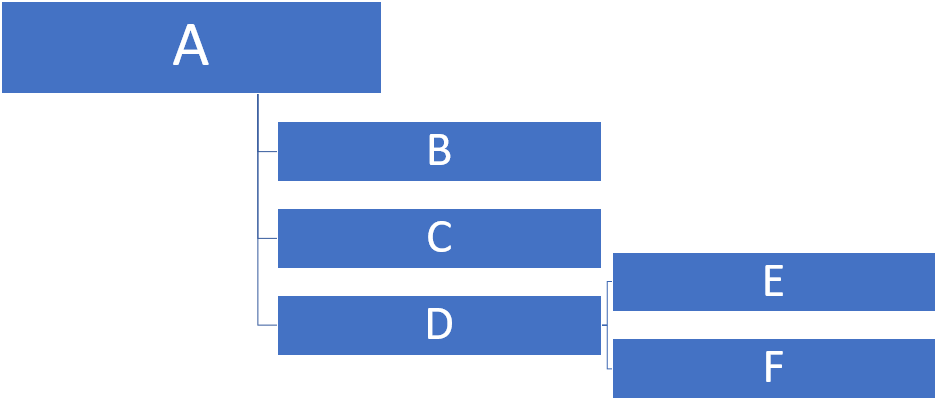
\includegraphics[width=10cm]{img/reddit_utterance_construction.PNG}
	\caption{Exemplary tree how the comment tree is structured for a single thread. A stands for the threads root node and B to F are comments.}
	\label{fig:data:reddit:utterance:construction}
\end{figure}

\section{Vocabulary and Coverage}
\label{data:word_coverage}
After the datasets for both corpora have been generated, we go on with generating corpus specific vocabularies. We do this by iterating the generated dataset and extracting all words which occur there. These collected words are then ranked by their frequency of occurence and converted into vocabularies containing the $n$ most used words, where $n$ stands for the number of words chosen. We decied that we would use three different vocabulary sizes: $25'000$, $50'000$ and $100'000$. As expected, the larger the vocabularies get, the better is the coverage.
\todo{tabelle word coverage ist nicht referenziert?}
\\
\begin{table}[H]
	\begin{adjustbox}{max width=\textwidth}
		\centering
		\small
		\begin{tabular}{lcccccc}
			\toprule
			&\specialcell{Size\\ {[Thousand]}}
			&\specialcell{No. of Words\\ {[Thousand]}}
			&\specialcell{No. of known Words\\ {[Thousand]}}
			&\specialcell{Perc. of known Words \\ {[\%]}}
			&\specialcell{No. of unknown Words \\ {[Thousand]}}
			&\specialcell{Perc. of unknown Words \\ {[\%]}}\\
			\midrule
			OpenSubtitles	&$25$		&$2362$	&$2096$	&$88.73\%$ &$266$	&$11.27\%$\\
							&$50$		&$2362$	&$2116$	&$89.57\%$	&$246$	&$10.43\%$\\
							&$100$	&$2362$	&$2127$	&$90.03\%$	&$236$	&$9.97\%$\\\\
			Reddit		&$25$		&$1717$	&$1683$	&$98.00\%$	&$34$		&$2.00\%$\\
						&$50$		&$1717$	&$1699$	&$98.98\%$	&$17$		&$1.02\%$\\
						&$100$	&$1717$	&$1707$	&$99.42\%$	&$10$		&$0.58\%$\\
			\bottomrule
		\end{tabular}
	\end{adjustbox}
	\caption{Word coverage of differently sized vocabularies extracted from the generated datasets.}
	\label{tbl:data:split:corpus:analyze}
\end{table}

Below, in figure~\ref{fig:data:reddit:vocab:analyze}, you can find plot where it shows how much percentage of the words in an utterance is missing using the specified vocabulary. It shows that the coverage of the Reddit vocabularies is much bigger than the OpenSubtitles.\todo{Begründung? es befinden sich viele Sätze mehrfach im Datensatz.}

\begin{figure}[H]
	\minipage{0.5\textwidth}
	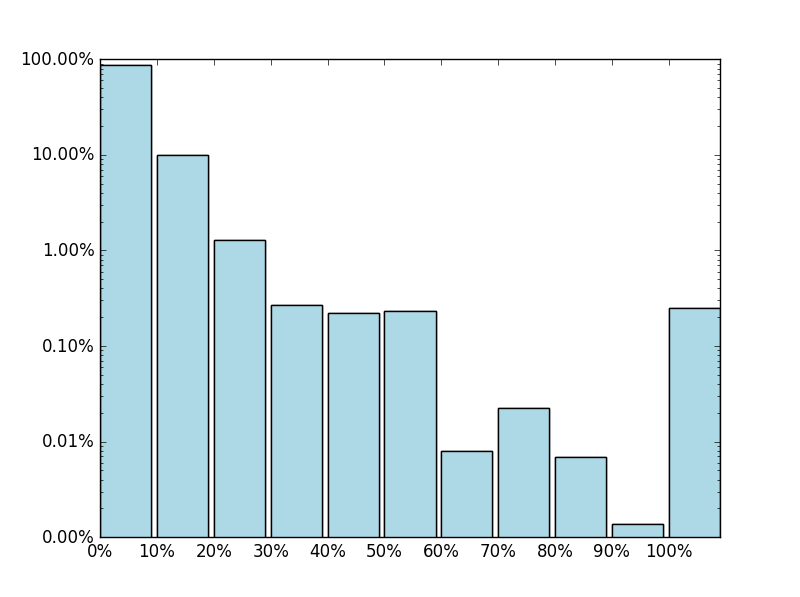
\includegraphics[width=\linewidth]{img/reddit_vocab_analyze_100k_perc.PNG}
	\centering
	\small
	\text{Reddit 100k}
	\endminipage\hfill
	\minipage{0.5\textwidth}
	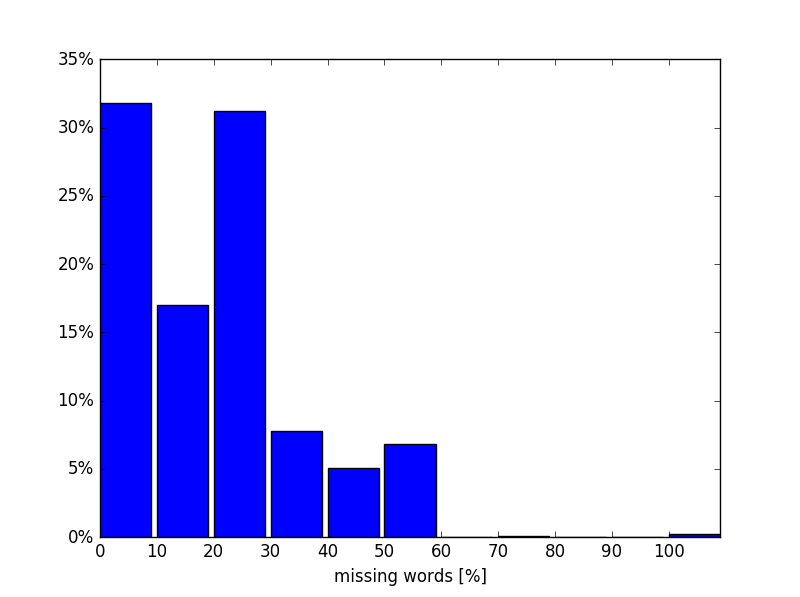
\includegraphics[width=\linewidth]{img/opus_vocab_analyze_100k_perc.PNG}
	\centering
	\small
	\text{OpenSubtitles 100k}
	\endminipage\hfill
	\minipage{0.5\textwidth}
	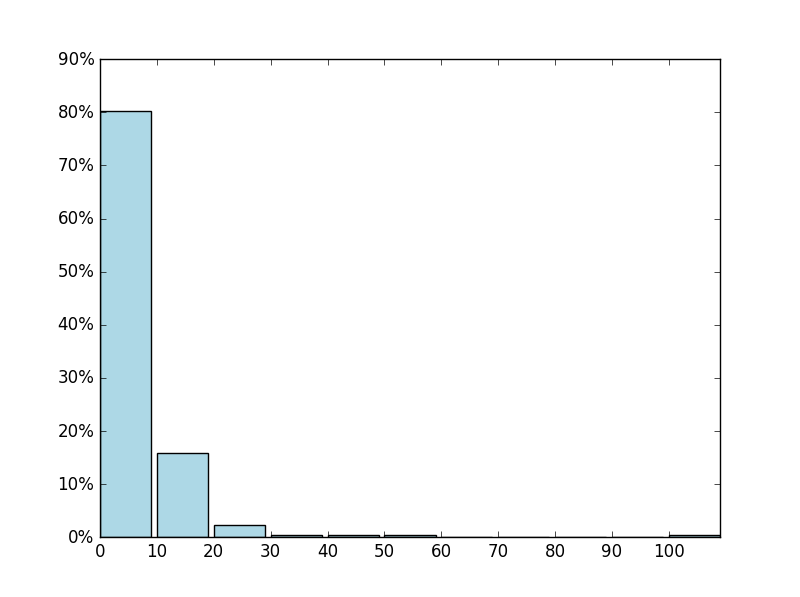
\includegraphics[width=\linewidth]{img/reddit_vocab_analyze_50k_perc.PNG}
	\centering
	\small
	\text{Reddit 50k}
	\endminipage\hfill
	\minipage{0.5\textwidth}
	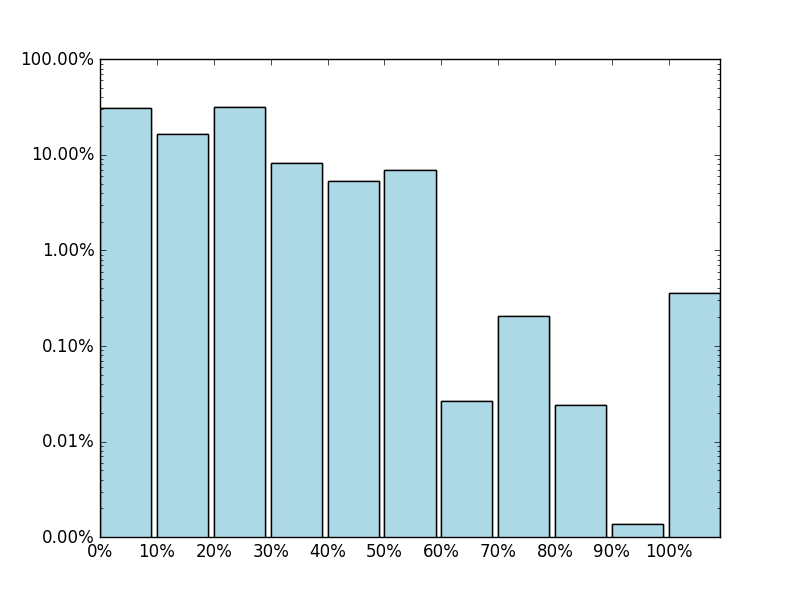
\includegraphics[width=\linewidth]{img/opus_vocab_analyze_50k_perc.PNG}
	\centering
	\small
	\text{OpenSubtitles 50k}
	\endminipage\hfill
	\minipage{0.5\textwidth}%
	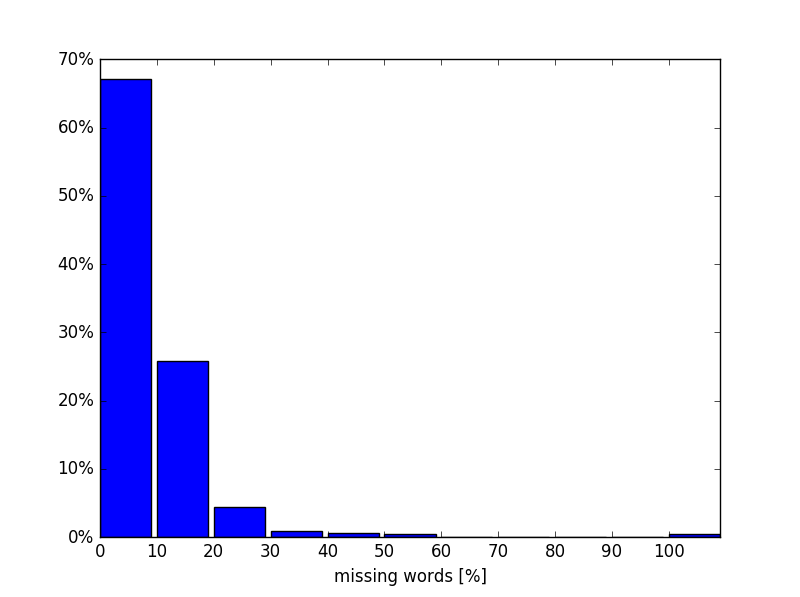
\includegraphics[width=\linewidth]{img/reddit_vocab_analyze_25k_perc.PNG}
	\centering
	\small
	\text{Reddit 25k}
	\endminipage\hfill
	\minipage{0.5\textwidth}%
	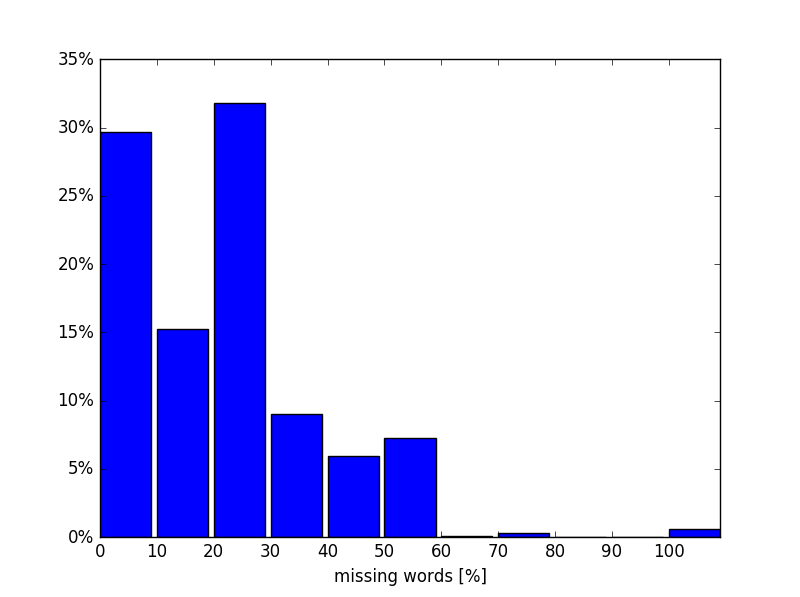
\includegraphics[width=\linewidth]{img/opus_vocab_analyze_25k_perc.PNG}
	\centering
	\small
	\text{OpenSubtitles 25k}
	\endminipage
	\caption{Plots showing the percentage of words missing per utterance for specific vocabulary sizes.}
	\label{fig:data:reddit:vocab:analyze}
\end{figure}
\todo{Other blue color and replace "missing words" with "Missing Words"}

\section{Splitting the Datasets}
\label{data:split_corpus}
The generated datasets have to be split in order to obtain a train, validation and test set. The table \ref{tbl:data:split:corpus} shows how proportions in which the datasets were split. We split in a way, that we always process two utterances at one to ensure that there is no overlap between the training and the other datasets. The splitting is also done randomly, to ensure that we do not run into problems due to the fact that the utterances may be sorted in any unknown way.
\\
\begin{table}[H]
	\centering
	\begin{adjustbox}{max width=\textwidth}
		\centering
		\small
		\begin{tabular}{llccc}
			\toprule
			&  \specialcell{Set}
			&  \specialcell{Share of Dataset \\ {[\%]}}
			&  \specialcell{Size \\{[MB]}}
			&  \specialcell{No. of Lines \\{[Thousand]}}\\
			\midrule
			OpenSubtitles	& Train	&97\%	&9'393	&321'643	\\
			&Valid	&1\%	&97		&3'315	\\
			&Test	&2\%	&194	&6'631	\\\\
			Reddit			&Train	&97\%	&8'455	&75'297	\\
			&Valid	&2\%	&185	&1'552	\\
			&Test	&1\%	&92		&776	\\
			\bottomrule
		\end{tabular}
	\end{adjustbox}
	\caption{Proportion in which the datasets were split to obtain a train, validation and test set.}
	\label{tbl:data:split:corpus}
\end{table}

\section{Time-Lag Analysis OpenSubtitles}
\label{data:opensubtitles:time_lag_analysis}
While searching through the OpenSubtitles dataset, we discovered that there are several pairs of utterances which don't make a lot of sense (e.g. (``I love cupcake'', ``Hello, how are you?'')) under the viewpoint of conversational modeling. We quickly realized that this useless pairs of utterances occur because of the way we preprocess the raw corpus: In order to get a sample, we take the first utterance and combine it with the utterance on the next line in the preprocessed corpus. The problem occurs there, where the timestamps signify a large time difference between the first and second utterance. This is comprehensible, as all utterances are just saved in the corpus one after each other without taking the timestamps (see OpenSubtitles paragraph in Chapter~\ref{data:structure_of_corpora}) into account. In order to investigate if this problem is urgent, we did an analysis to see if a large portion of the utterances have a time-lag higher than a certain timespan. The results of this investigation are summarized in the figure~\ref{fig:data:analyse:timediff:opus}.

\begin{figure}[H]
	\centering
	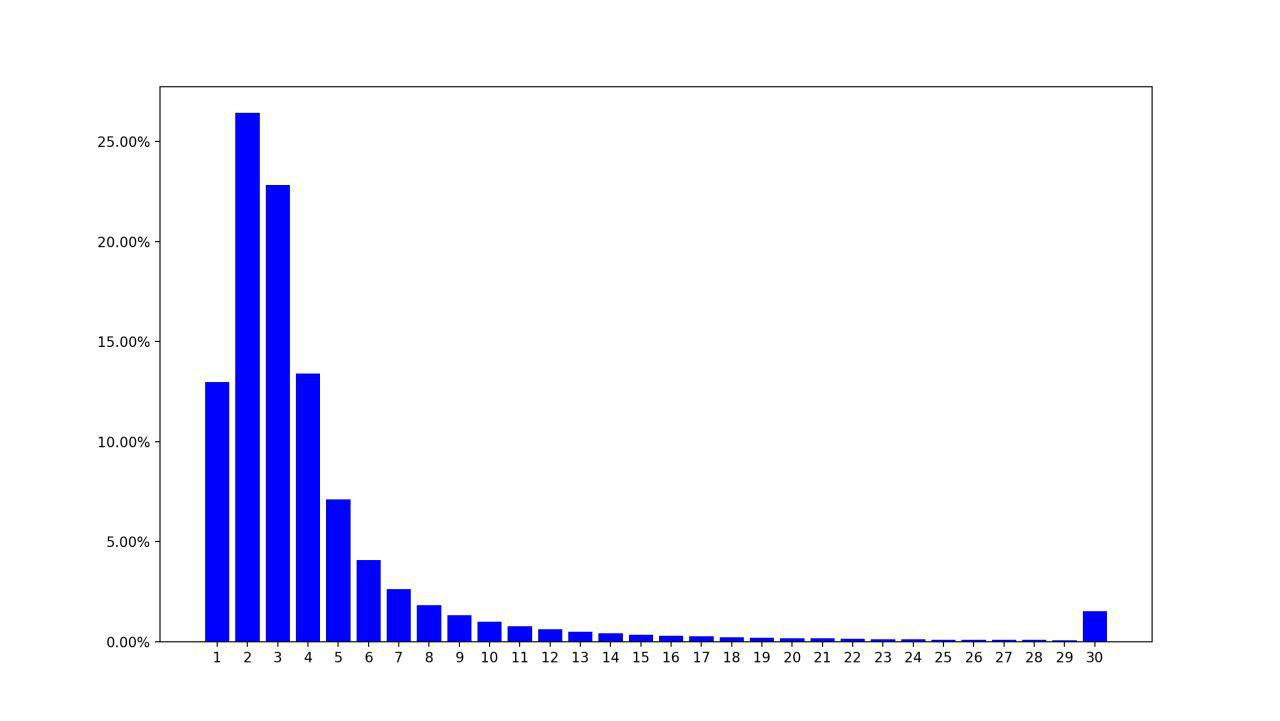
\includegraphics[width=15cm]{img/opus_time_analyze.PNG}
	\caption{Relative distribution (discrete) of the time-lag between two utterances in the raw OpenSubtitles corpus. Most of the utterances lie in the range from $1$ to $5$ seconds: $13.0\%$ within 1 second, $26.4\%$ within 2 seconds, $22.8\%$ within 3 seconds, $13.4\%$ within 4 seconds and  $7.0\%$ within 5 seconds.}
	\label{fig:data:analyse:timediff:opus}
\end{figure}

As one can see, most of the utterances, actually over 80\%, occur between $1$ and $5$ seconds after each other. The \todo{big? oder einfach nur spike?}big spike at the end of the graph contains a much large portion than all the other between $10$ and $30$ seconds. This has to do with the fact, that there might be changes in the scenes of the movies, which can lead to two consecutive utterances in the corpus being uttered with a larger time gap. The other reason is, that each movie is stored in a single file and hence, there might be utterances which are combined, but actually belong to two different movies.

As this analysis has shown, most of the utterances lie so close to each other, that this will most probably not be a problem when training our model with it.

\section{N-Gram Analysis}
\label{chapter:data:ngram}
We also do an n-gram analysis of the used corpora. For this purpose, we generated uni- and bigrams for both the OpenSubtitles and Reddit corpora. We do this, to be able to compare the n-grams of the outputs produced by our models after they have been trained with the n-grams obtained when analyzing the preprocessed corpora. This enables us to find correlations between the n-grams produced by this analysis and n-grams extracted from the outputs of the trained models. The results of analyzing the preprocessed datasets are visualized in the figures~\ref{data:ngram:freq_top_30} and \ref{data:ngram:graph_top_50}. For the second visualizations, we use a custom graph visualization which we call ``N-Gram Graph''. This allows us to visualize how n-grams can be connected to each other (through edges) and at the same time visualize their relative occurrence frequencies to all other n-grams in the graph.
 
\begin{figure}[H]
	\minipage{0.5\textwidth}
	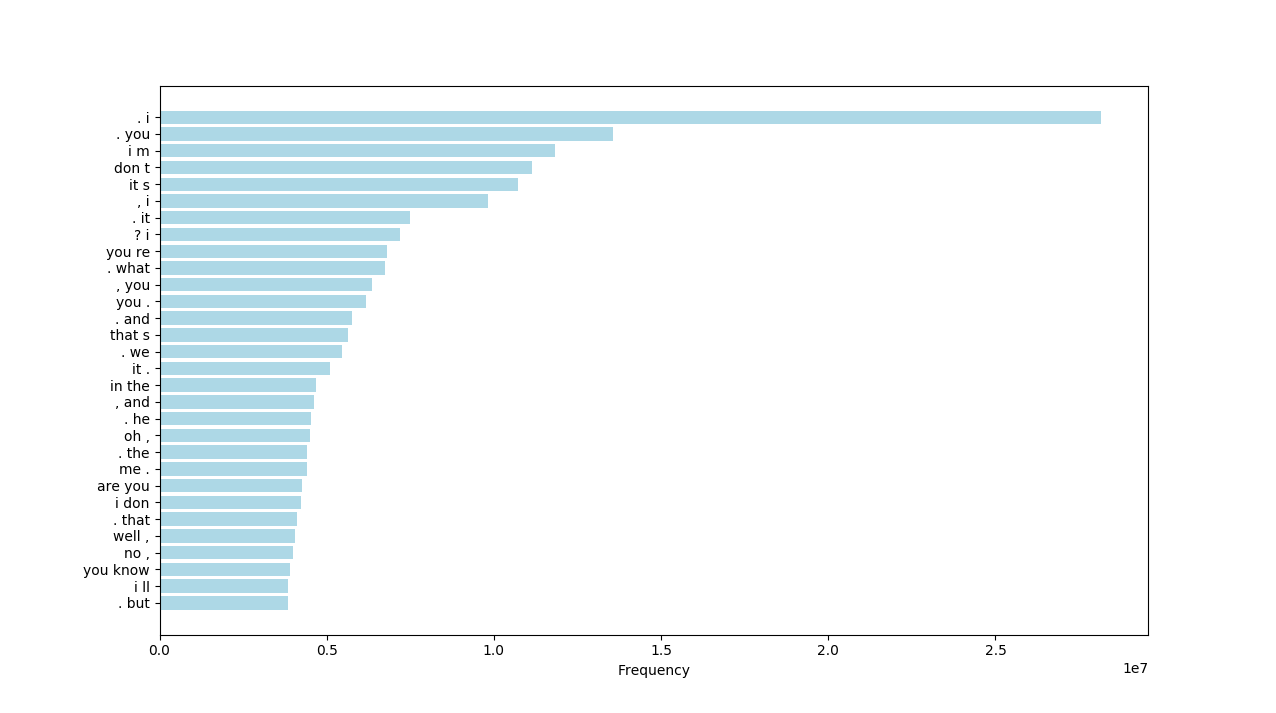
\includegraphics[width=\linewidth]{img/opensubtitles_bigram_top_30_freq}
	\centering
	\small
	\text{OpenSubtitles}
	\endminipage\hfill
	\minipage{0.5\textwidth}
	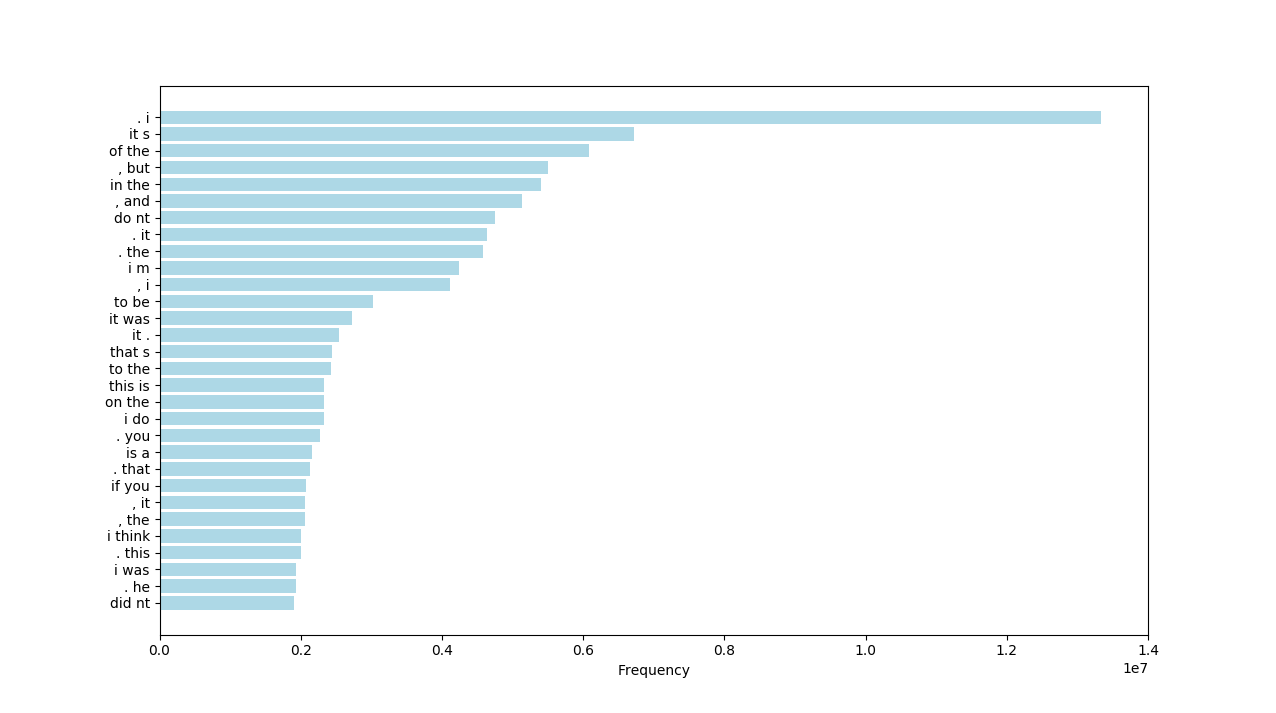
\includegraphics[width=\linewidth]{img/reddit_bigram_top_30_freq}
	\centering
	\small
	\text{Reddit}
	\endminipage\hfill
	\caption{Occurrence frequencies of the 30 most used bigrams in the OpenSubtitles~(left) and Reddit (right) datasets.}
	\label{data:ngram:freq_top_30}
\end{figure}

\begin{figure}[H]
	\minipage{1\textwidth}
	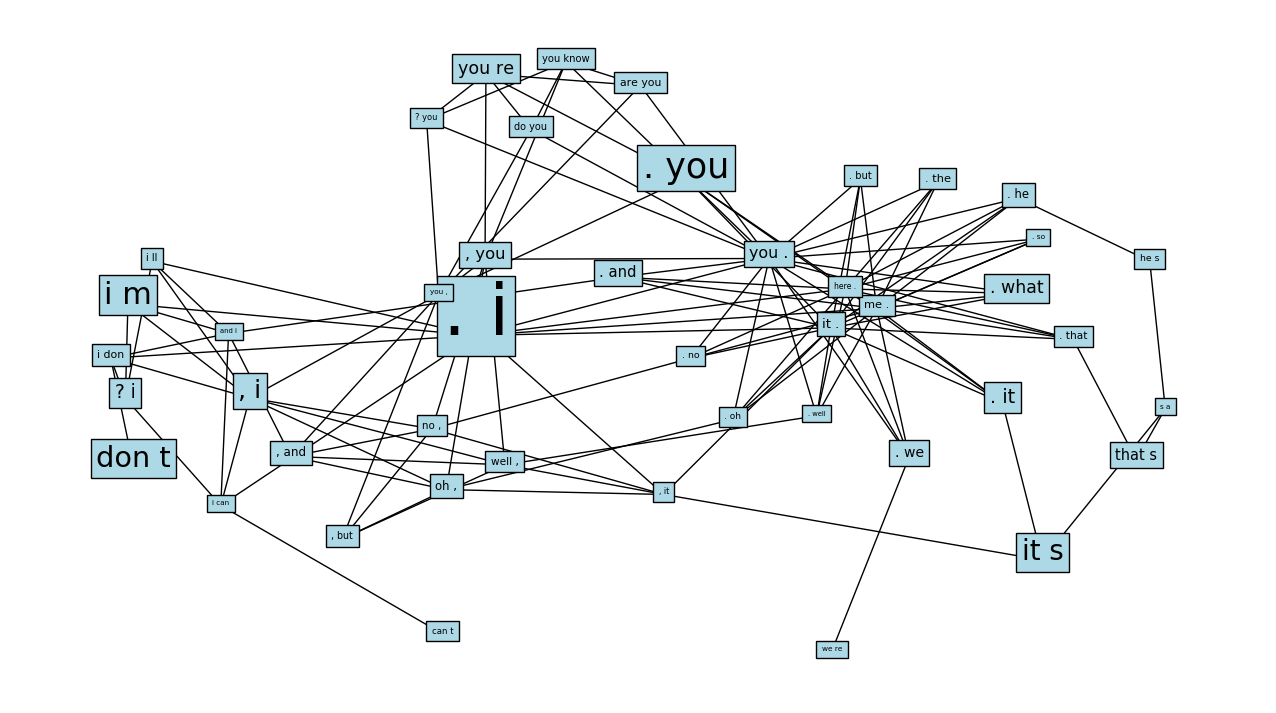
\includegraphics[width=\linewidth]{img/opensubtitles_bigram_top_50_graph}
	\centering
	\small
	\text{OpenSubtitles}
	\endminipage\hfill
	\minipage{1\textwidth}
	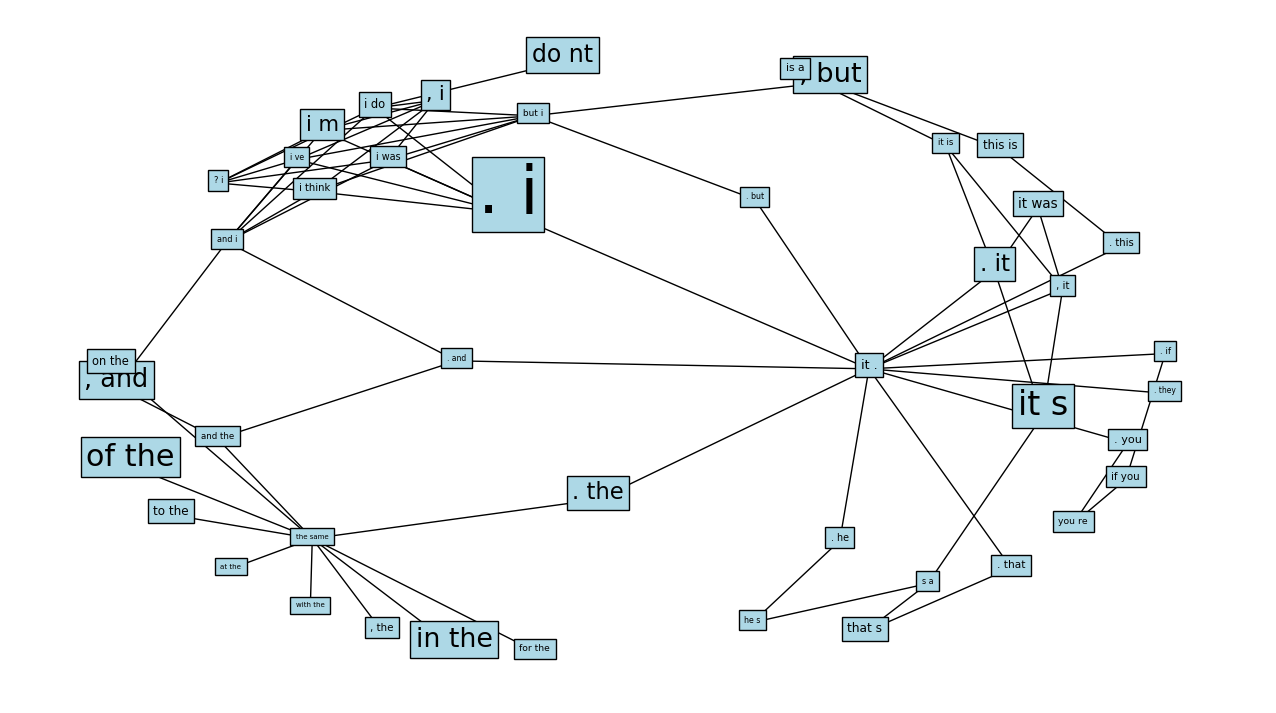
\includegraphics[width=\linewidth]{img/reddit_bigram_top_50_graph}
	\centering
	\small
	\text{Reddit}
	\endminipage\hfill
	\caption{N-Gram graphs for the 50 most used bigrams in the OpenSubtitles (upper) and Reddit (lower) datasets. Each node in the graphs represents a bigram, the edges between them show that either the first word of the first bigram matches the second word of the other bigram or the last word of the first bigram equals the last word of the second bigram. The size of each node is relative to its occurrence frequency, which means, that larger nodes occur more frequent than smaller ones.}
	\label{data:ngram:graph_top_50}
\end{figure}


\chapter{Methods}
\label{methods}
In the following chapter, we are going to elaborate on how we performed the experiments, which hyperparameters where used and how we evaluated the results of the trained models.

\section{Architecture of the Sequence-To-Sequence Model}
In the following paragraphs, we are going to describe the architecture of the model used to conduct our experiments.

\paragraph{Sequence-To-Sequence} In general, we are using the architecture of seq2seq models describe in chapter \ref{fundamentals:seq2seq}. We are using LSTM cells. We restrict ourselves to only use one LSTM cell for the encoder, and another cell for the decoder. This has to do with the fact, that we wanted our cells to be as large as possible to come as close to the size of the cells used in \cite{Vinyals:2015}, as we are trying to replicate the results from there. However, this is not simply possible due to the fact, that in the referenced paper, they used two really large cells with each having a hidden state size of $4096$ hidden units and a vocabulary consisting of $100'000$ words. In the paper, they trained their models on a CPU due to this fact, because such a huge network fits does not fit in the memory of any GPU currently available. As we are seeking to train our models on a single GPU (see chapter \ref{sofware_system:development_history}), we had to shrink the size of our model to the biggest size possible so that it still fits within the 12GB of memory the GPUs we are using have (see chapter \ref{software_system:hardware}). The exact size of the model used in this thesis is described in the subsequent paragraph ``Hyperparameters'' below.

\paragraph{Down-Projection of Hidden State} Because of the problematic with such large RNN cells as described in the preceding paragraph, we implemented a so-called \emph{down-projection} at the end of the decoder cell. This is done similar to the down-projection used in \cite{Vinyals:2015}, with the main difference lying in the motivation why we implemented it. In the paper, they state, that they used it to speed up the training due to the large weights-matrix in the softmax layer at the end. In our case, the down-projection was not just for speeding up the training, but mainly to allow us to use bigger cells than we would be able to without the projection. The implementation of this feature allowed us to grow our model in size by a factor of $2$, from a hidden state size of $1024$ to $2048$, without the need to sacrifice the size of the vocabulary used (see chapter \ref{methods:hyperparameters} for more informations on the used hyperparameters).

\paragraph{Sampled Softmax} To speed up the training of the large softmax layer at the end (consisting of $50'000$ entries), we use a \emph{sampled softmax} as described in \cite{Sebastien:2014} which is only applied while training the models. Basically, the idea behind it is, that instead of using the full softmax at each time step in the decoder, we only use a subset of the words which is randomly sampled (besides the words which is the target word) from the vocabulary to approximate the softmax layer. This speeds up training dramatically \todo{Descirbe more!}. On inference time, we then have to use the full softmax layer again to generate the predictions.

\paragraph{Static Unrolling of RNN} Due to the fact, that we are working with a deprecated \texttt{TensorFlow} API (see chapter \ref{sofware_system:development_history}), we have to use static unrolling for our model. Static unrolling works, by defining a fixed size of time steps for the encoder and decoder, and then unrolling the encoder and decoder cell for this number of time steps \emph{before} we are actually computing anything using it. This actually ``removes'' the recurrence from our model and transforms it into kind-of ``feed forward'' model with the major difference being, that the weights are shared between the layers of the unrolled model (as each layer basically represents the same cell).

\begin{figure}
	\label{methods:static_unrolling:unrolled_rnn}
	\centering
	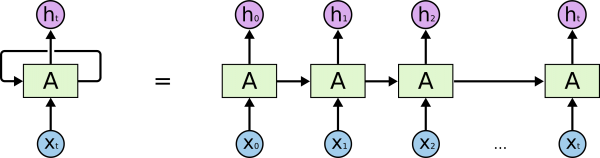
\includegraphics[width=10cm]{img/rnn_unrolled}
	\caption{Image for illustrating the process of unrolling an RNN over a fixed size of time steps.\protect\footnotemark}
\end{figure}
\footnotetext{http://colah.github.io/posts/2015-08-Understanding-LSTMs/}

This implementation forced us to define a maximum number of time steps used for the encoder and decoder beforehand.

\section{Hyperparameters}
\label{methods:hyperparameters}

\paragraph{Model} In summary, for our model we are using the following hyperparameters:

\begin{table}[H]
	\centering
	\ra{1.3}
	\begin{adjustbox}{max width=\textwidth}
		\begin{tabular}{ll}
			\toprule
			Name & Value\\ \midrule
			Number of encoder cells & $1$\\
			Number of decoder cells & $1$\\
			Max. number of time steps in encoder & $30$\\
			Max. number of time steps in decoder & $30$\\
			Hidden state size & $2048$\\
			Projected hidden state size & $1024$\\
			Number of sampled words for softmax & $512$\\
			Size of the softmax layer & $50'000$\\
			\bottomrule
		\end{tabular}
	\end{adjustbox}
	\caption{Hyperparameter, which were used for our seq2seq model.}
	\label{methods:hyperparameters:table}
\end{table}

\paragraph{Optimizer} As the optimizer, we used \emph{AdaGrad} \cite{Duchi:2011} as in \cite{Vinyals:2015} with the learning rate set to $0.01$. We also use gradient clipping and set the maximum allowed gradient value to be $10$, as described in \cite{Pascanu:2013}.

\paragraph{Training} We trained our models on the hardware described in chapter \ref{software_system:hardware} with the software packages from \ref{software_system:softwar_packages}.

\section{Evaluation}
\blindtext

\chapter{Analysis of Results}
We are going to analyze the resulting models after training them as specified in Chapter~\ref{methods:training}.

In the first part, we are going to analyze how the training went and review the results of the metric-based evaluation (see Chapter~\ref{methods:evaluation}). Because we identified some problems with this quantitative analysis, we then show that progress was indeed achieved throughout the training and explore why the results of the evaluation are as poor as they are. This includes an analysis of the language model to determine why the models often respond with generic outputs.

The next part is dedicated to the comparison of our models with the results from the paper of Vinyals and Le~\cite{Vinyals:2015} and with the CleverBot chatbot.

The subjects of the last part are the analyzes analysis related beam-search, the soft-attention mechanism and the clustering of thought vectors.

\section{Was the Training Successful?}
First, we start by analyzing the evolution of the models with regard to the available performance metrics throughout the time period of the training. Below, in Figures~\ref{results:learning_process:metrics:opensubtitles} and~\ref{results:learning_process:metrics:reddit}, the development of the cross-entropy loss and perplexity values on the training datasets for the two different models is depicted.

\paragraph{OpenSubtitles} It is eye-catching when comparing the two models that the OpenSubtitles apparently has much more variance in its performance on the validation dataset in comparison to the Reddit model. This is most probably caused by the fact that the OpenSubtitles dataset is much more noisey than the Reddit dataset, as also noticed by others~\cite{Vinyals:2015}. This is related to the missing information about turn taking, which means it is certainly possible that consecutive utterances in the dataset may be uttered by the same person even though we treat it if they were uttered by two different persons. Also, there is the issue with the time lags between utterances as analyzed in Chapter~\ref{data:opensubtitles:time_lag_analysis}. In contrast, with the Reddit dataset we always know who uttered a comment and hence can build a dataset which ensures that the dialogs make sense from a structural perspective.

\begin{figure}[H]
	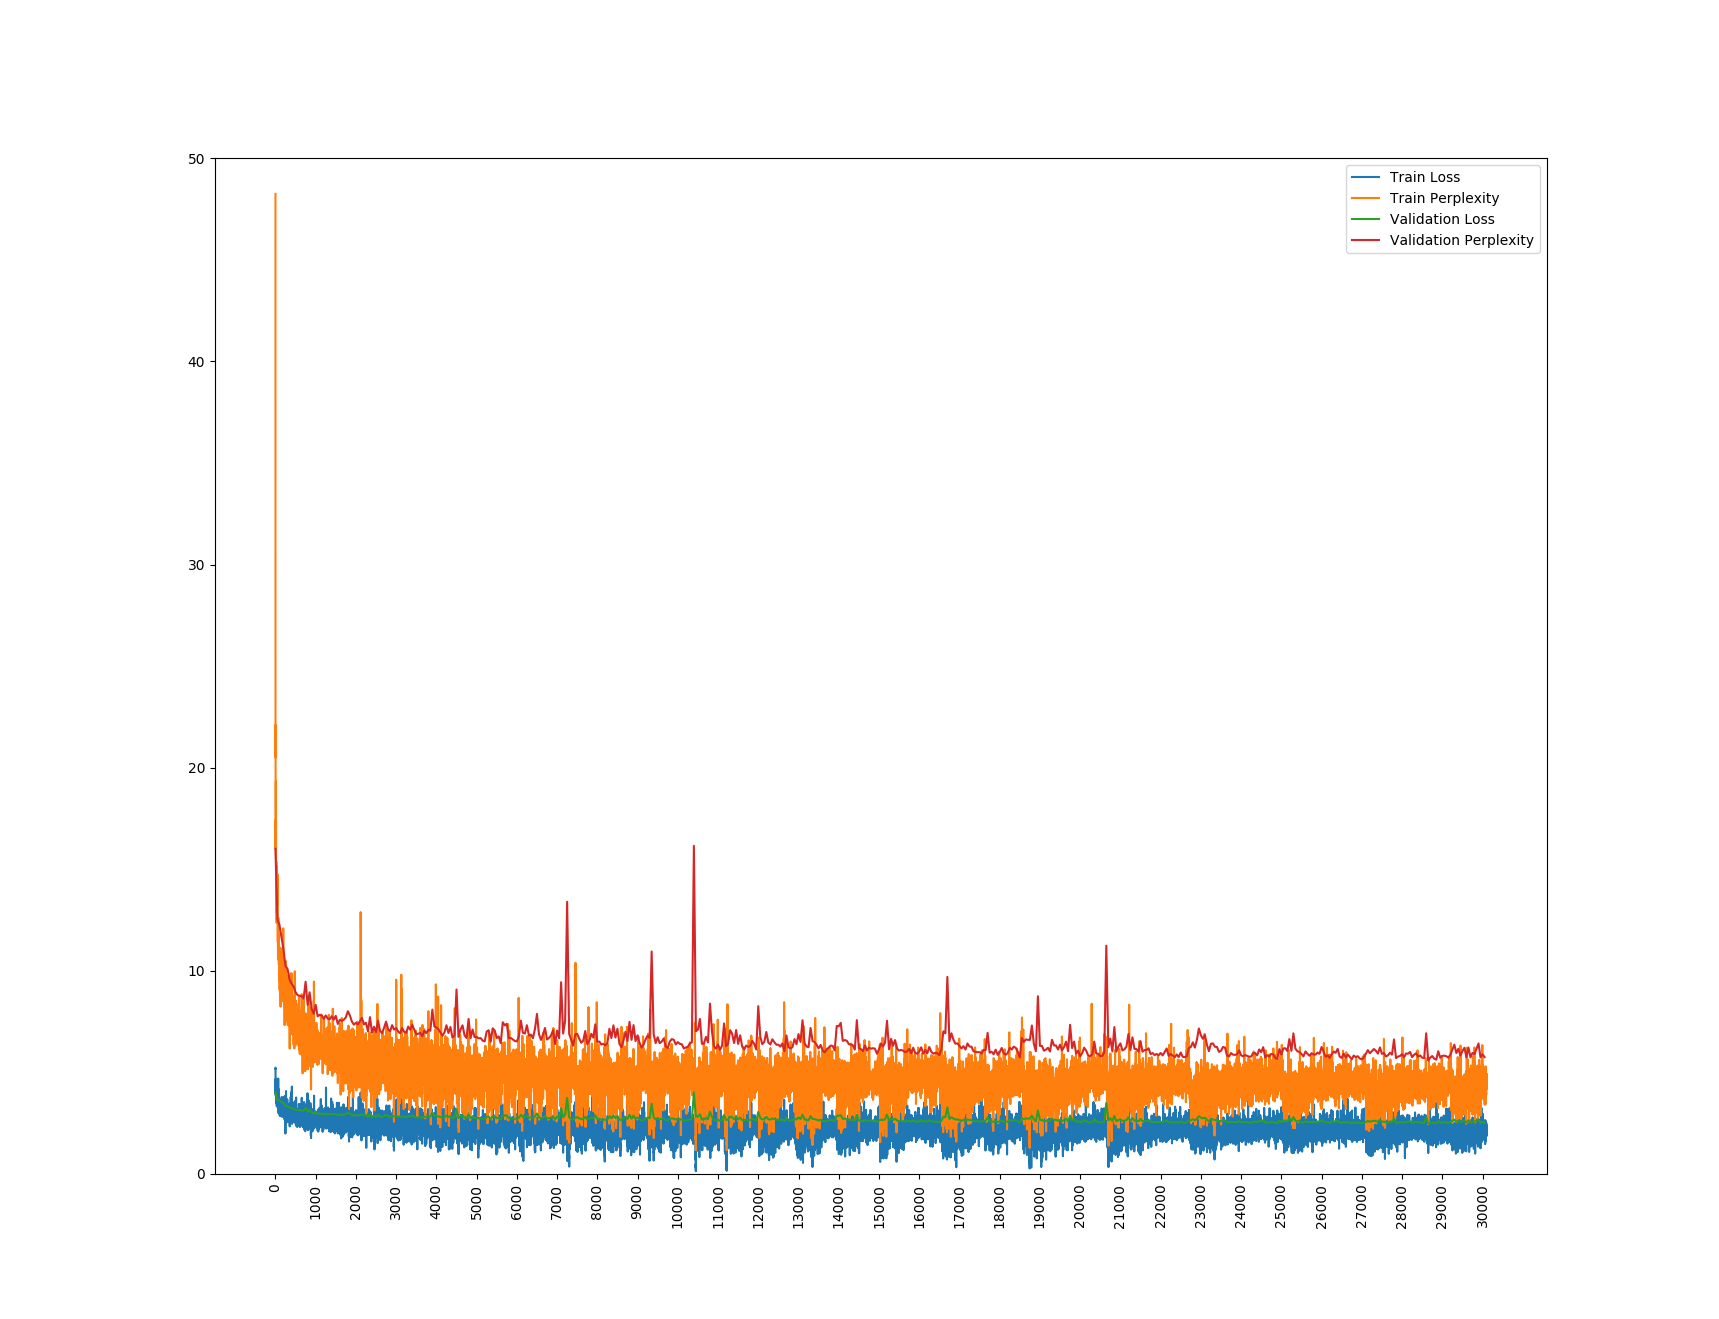
\includegraphics[width=\linewidth]{img/plots/opensubtitles_not_reversed/train_metrics.png}
	\caption{Development of the loss and perplexity values on the training and validation datasets throughout the training of the OpenSubtitles model. One tick on the x-axis is equal to $100,000$ batches processed.}
	\label{results:learning_process:metrics:opensubtitles}
\end{figure}

\paragraph{Reddit} The learning process of the Reddit model looks appropriate, but it also has a peculiarity, namely the dips in the training loss and perplexity. These dips occur about every $300,000$ to $400,000$ batches. They are also present in the development of the validation loss and perplexity, but are not as apparent as in the metrics on the training dataset. We currently cannot explain this behavior. We assume that this peculiarities are caused by the structure of the training dataset.\todo{Maybe explain a little bit more?} However, the variance is much smaller than with the OpenSubtitles model, which strengthens our argument that well-structured datasets are indeed favorable when training such systems as helps to avoid confusion due to perplexing samples.

\begin{figure}[H]
	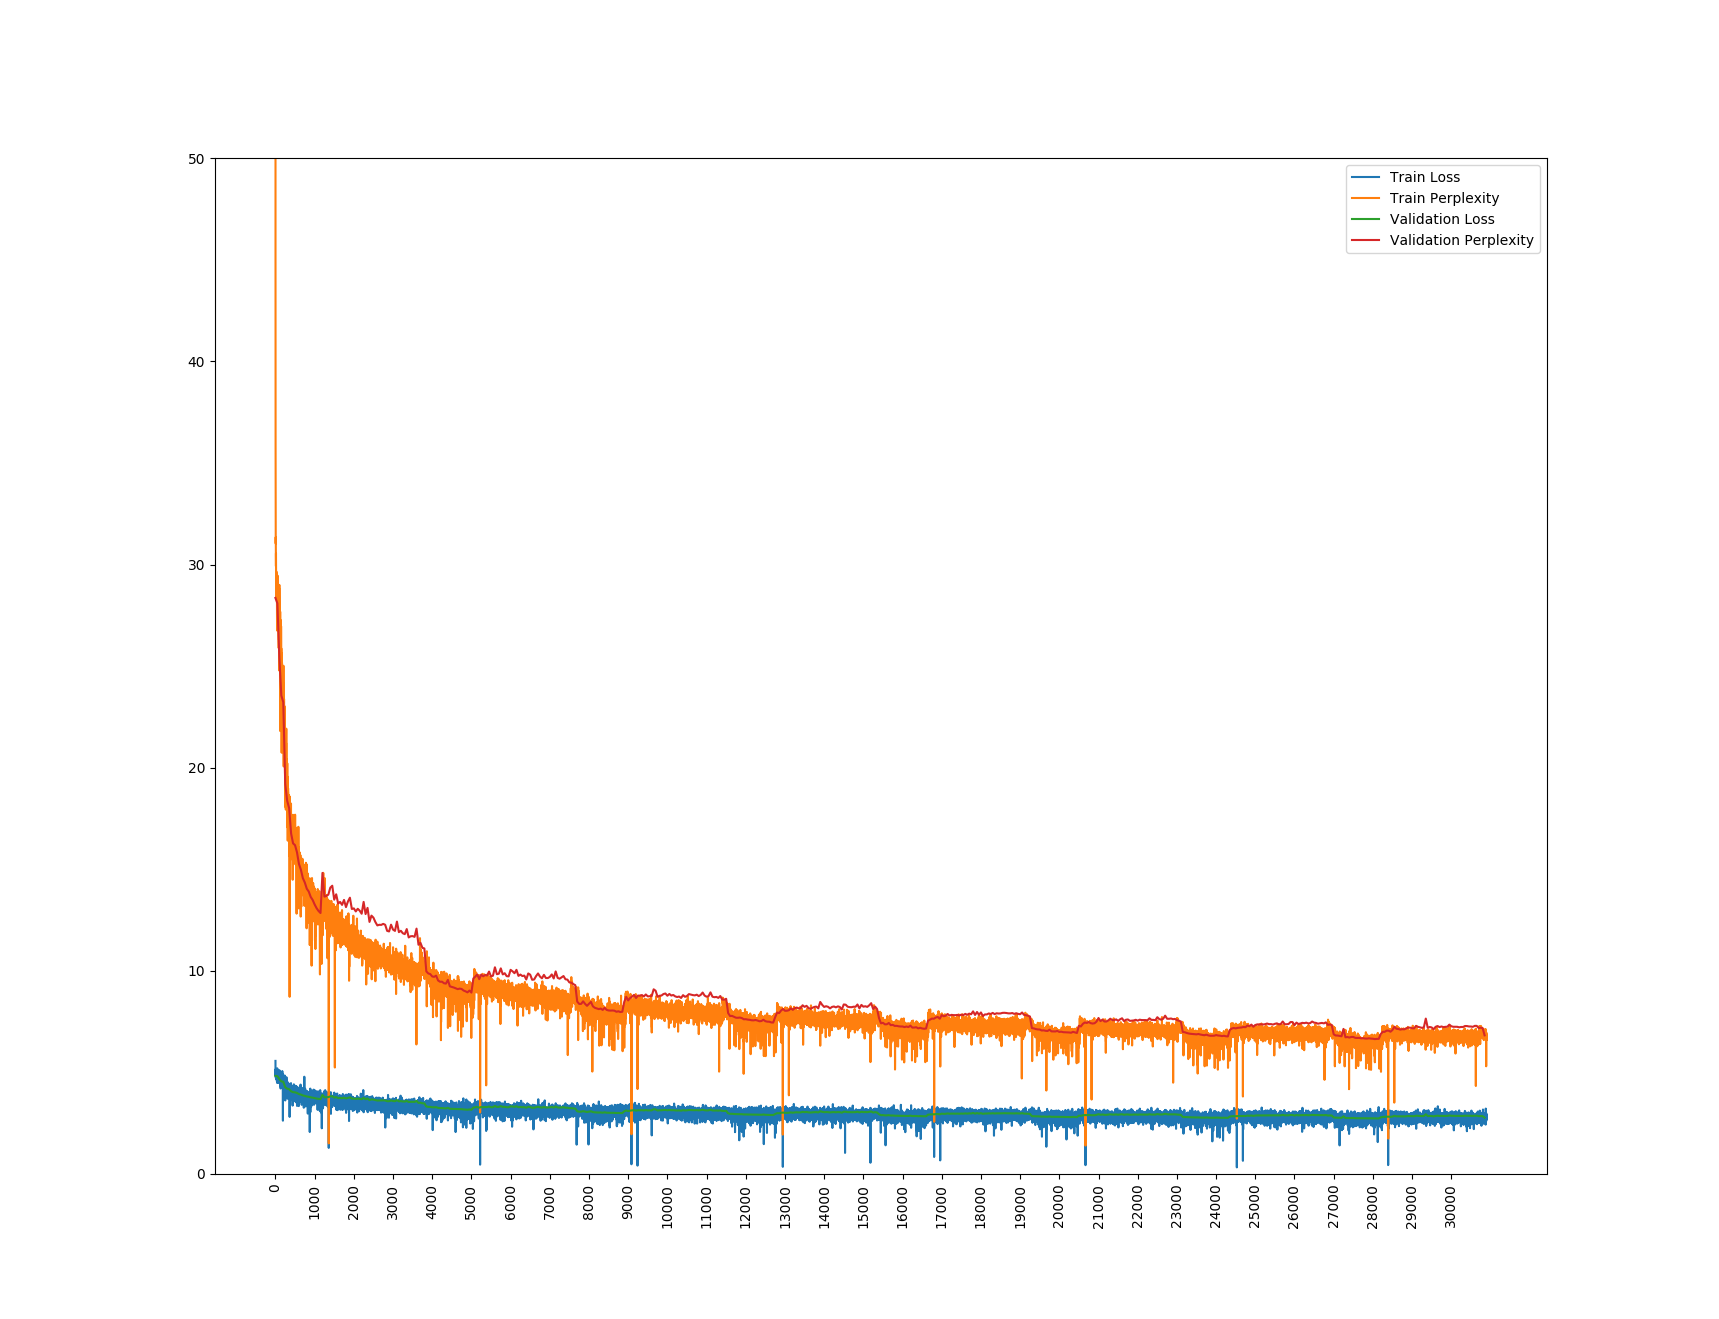
\includegraphics[width=\linewidth]{img/plots/reddit/train_metrics.png}
	\caption{Development of the loss and perplexity on the training and validation datasets throughout the training of the Reddit model. One tick on the x-axis is equal to $100,000$ batches processed.}
	\label{results:learning_process:metrics:reddit}
\end{figure} 

\paragraph{The Training Seems Successful} From the appearance of the plots, it looks like the training went fine for both models, as both of them exhibit degrading loss and perplexity values. We see differences in how the models have evolved over the time span of the training, but we cannot derive any conclusion at the current time. After we have analyzed the training process, we are now focusing on the performance of the models on the test datasets.

\section{Performance on Test Datasets}
\label{results:performance_on_test_datasets}
After we have seen that the training process looks fine, we are going to assess the performance of these models on our test datasets. Here we use the same metrics as during the training, namely the cross-entropy loss and perplexity. We evaluate each model on the respective test dataset for each of the six snapshots we have created during training (see Chapter~\ref{methods:training}).

\paragraph{Surprising Results} The results on the test dataset are quite the opposite of the results of the training process (see Figures~\ref{result:test_performance:opensubtitles} and~\ref{result:test_performance:reddit}), the performance for both of the models is
worsening over time. The results of the OpenSubtitles model (see Table~\ref{results:test_metrics:opensubtitles}) vary across the different snapshots, with the best result having a perplexity of $71.07$ and a loss of $6.15$ and derived from the evaluation of the first snapshot. Also, the best result of the Reddit model (see Table~\ref{results:test_metrics:reddit}) is achieved on the first snapshot with a perplexity of $169.14$, with all other snapshots having a worse perplexity.
\\
\begin{table}[H]
	\centering
	\begin{adjustbox}{max width=\textwidth}
		\begin{tabular}{l|cc}
			\toprule
			Snapshot & Test Loss & Test Perplexity\\
			\midrule
			0.5M & $6.1513$ & $71.0779$\\
			1.0M & $6.5314$ & $92.5000$\\
			1.5M & $7.3942$ & $168.2207$\\
			2.0M & $6.2134$ & $74.2035$\\
			2.5M & $6.3627$ & $82.2949$\\
			3.0M & $6.4647$ & $88.3205$\\
			\bottomrule
		\end{tabular}
	\end{adjustbox}
	\caption{Loss and perplexity values for each snapshot of the OpenSubtitles model when evaluating it with the test dataset.}
	\label{results:test_metrics:opensubtitles}
\end{table}

\begin{table}[H]
	\centering
	\begin{adjustbox}{max width=\textwidth}
		\begin{tabular}{l|cc}
			\toprule
			Snapshot & Test Loss & Test Perplexity\\
			\midrule
			0.5M & $7.4021$ & $169.1432$\\
			1.0M & $7.5477$ & $187.1090$\\
			1.5M & $7.5794$ & $191.2557$\\
			2.0M & $7.6288$ & $197.9190$\\
			2.5M & $7.6661$ & $203.1056$\\
			3.0M & $7.7885$ & $221.0843$\\
			\bottomrule
		\end{tabular}
	\end{adjustbox}
	\caption{Loss and perplexity values for each snapshot of the Reddit model when evaluating it with the test dataset.}
	\label{results:test_metrics:reddit}
\end{table}

This result contradicts with our expectation. Instead increasing loss values, we would have expected it to decrease in the same way as it did on the training and validation datasets. We assume, that this is related to the cross-entropy loss and hence the perplexity being not the best fit metrics to evaluate such models, especially in a conversational context where the variety of correct answers can be extensive. We have no explanation, why the values on the validation dataset are getting better over time. For this reason, we propose a third performance metric, namely the usage of Sent2Vec~\cite{Pgj:2017} embeddings, to measure the similarity between the expected and generated responses. Before we perform this analysis, we want to take a look at different samples from both models to show that they indeed improved over time, even though the results of the test metrics tell a different story.\todo{Maybe rewrite this sentence because it sounds like we are debunking the bad metrics by simply playing with the models}

\begin{figure}[H]
	\minipage{0.5\textwidth}
	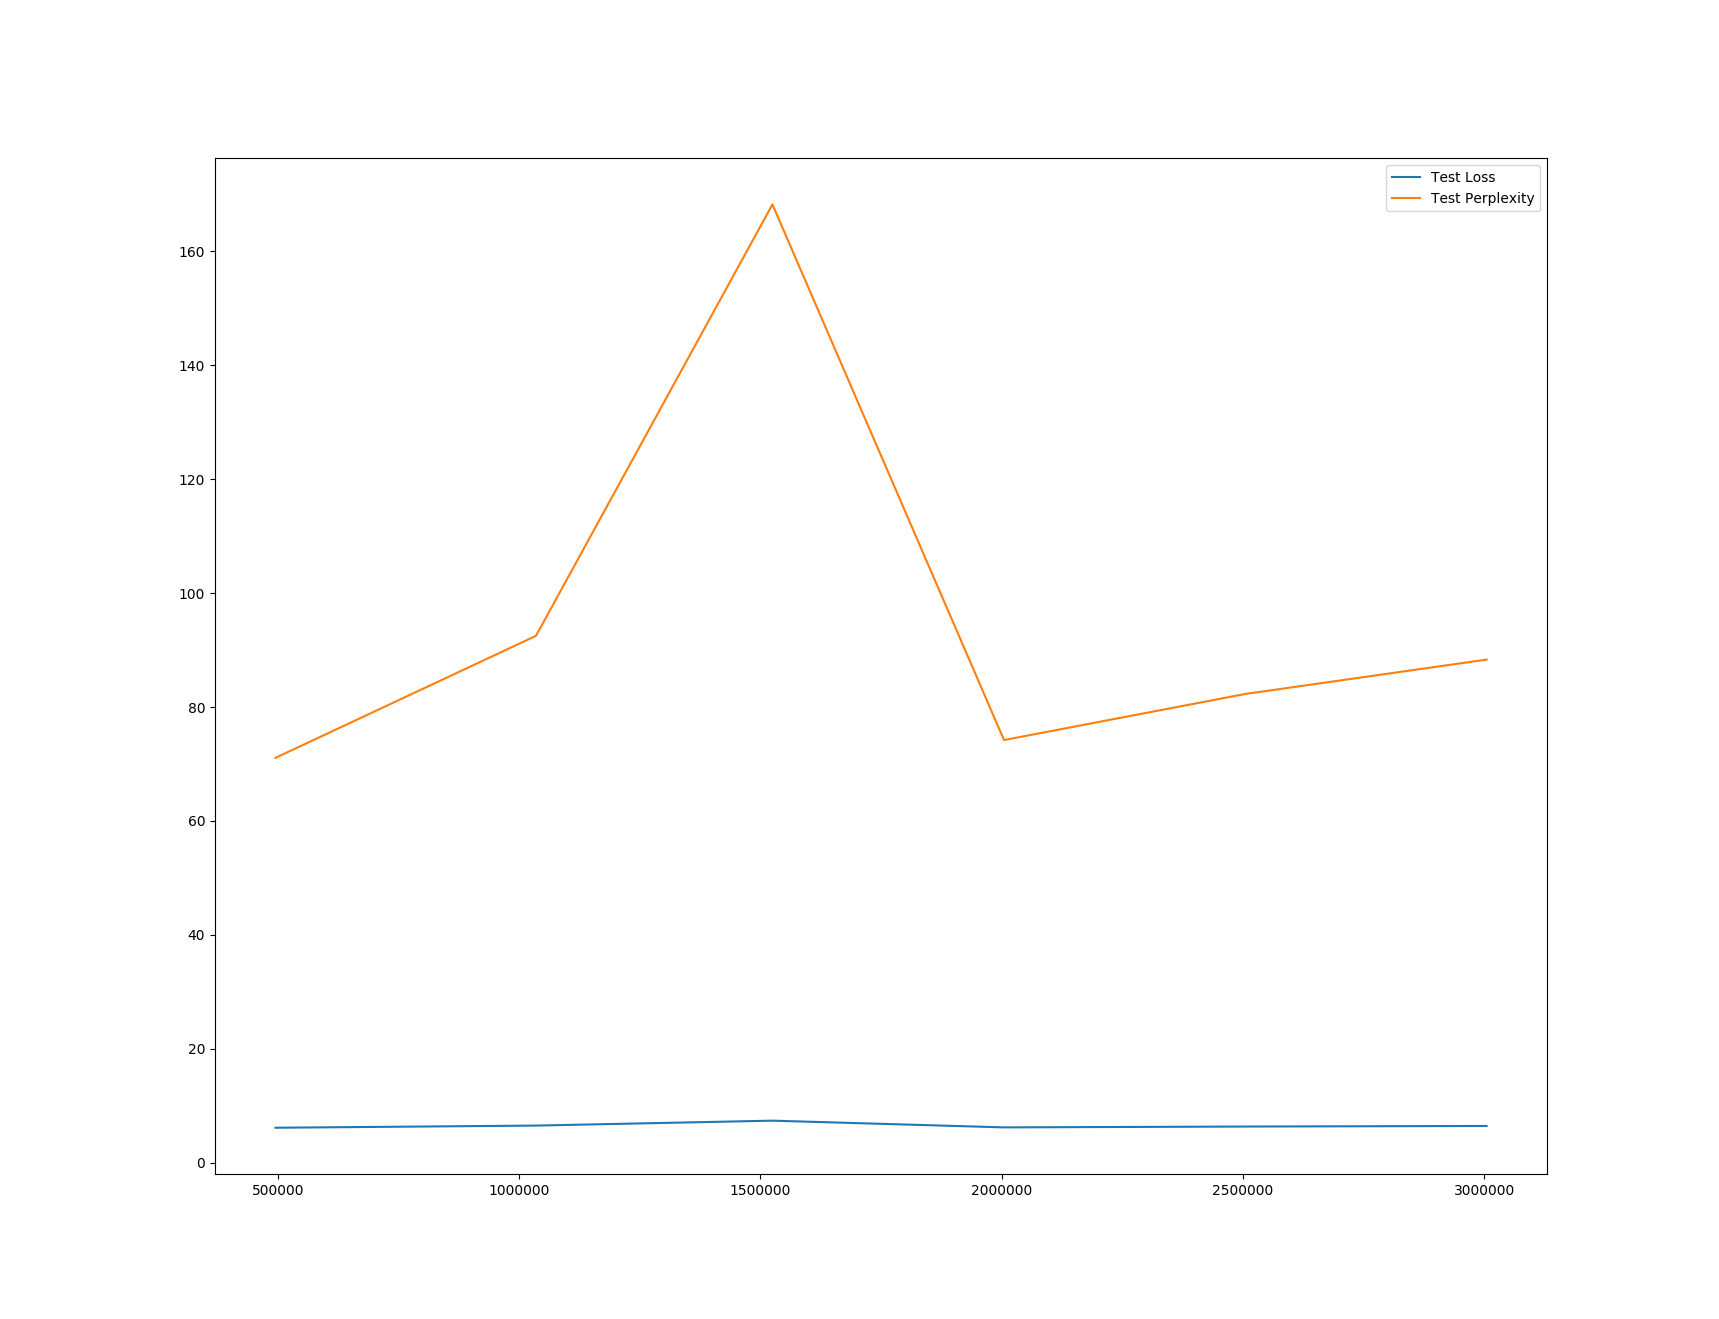
\includegraphics[width=\linewidth]{img/plots/opensubtitles_not_reversed/test_metrics_both.png}
	\centering
	\small
	\text{The loss and perplexity.}
	\endminipage\hfill
	\minipage{0.5\textwidth}
	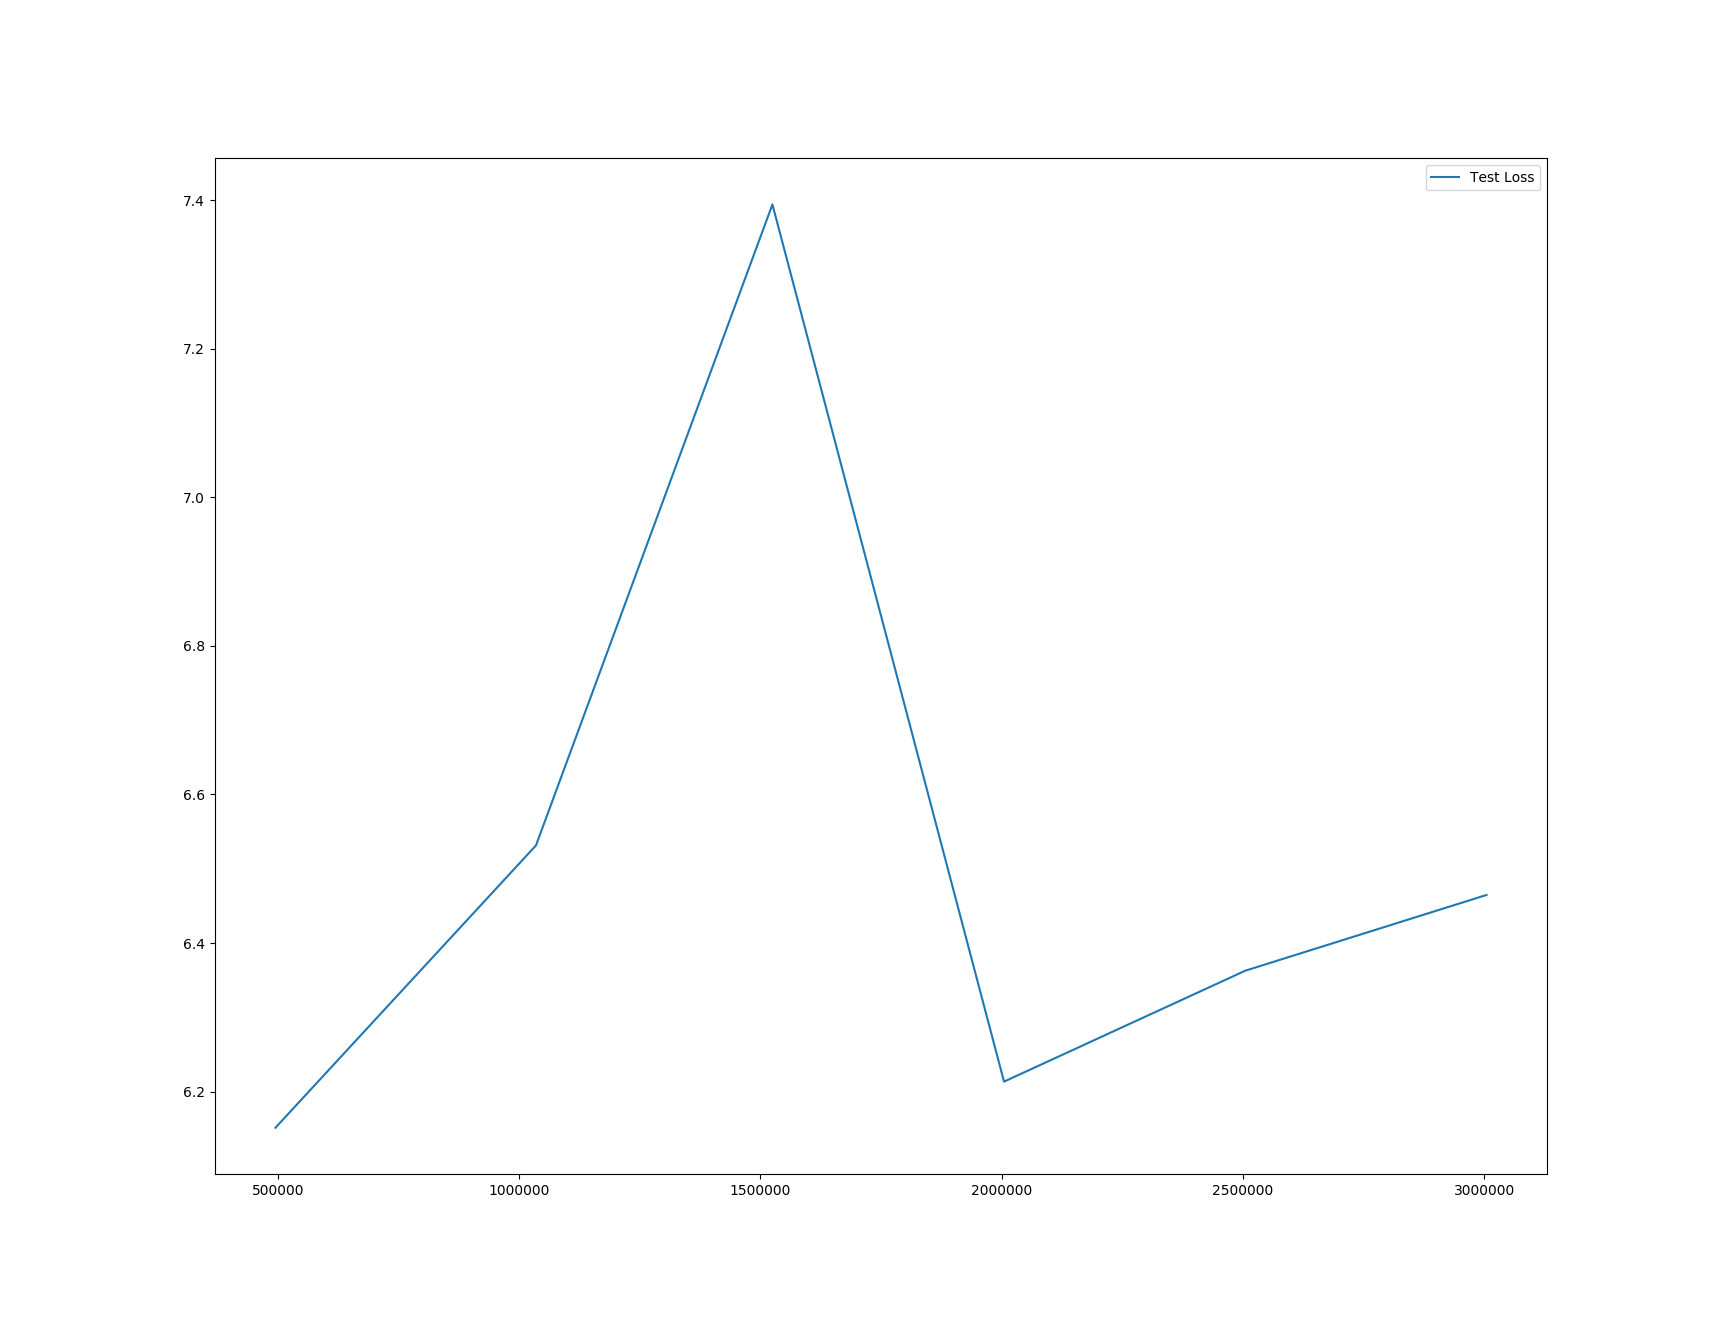
\includegraphics[width=\linewidth]{img/plots/opensubtitles_not_reversed/test_metrics_loss.png}
	\centering
	\small
	\text{Only the loss.}
	\endminipage\hfill
	\caption{The loss and perplexity when evaluating the six different snapshots with the test dataset using the OpenSubtitles model.}
	\label{result:test_performance:opensubtitles}
\end{figure}

\begin{figure}[H]
	\minipage{0.5\textwidth}
	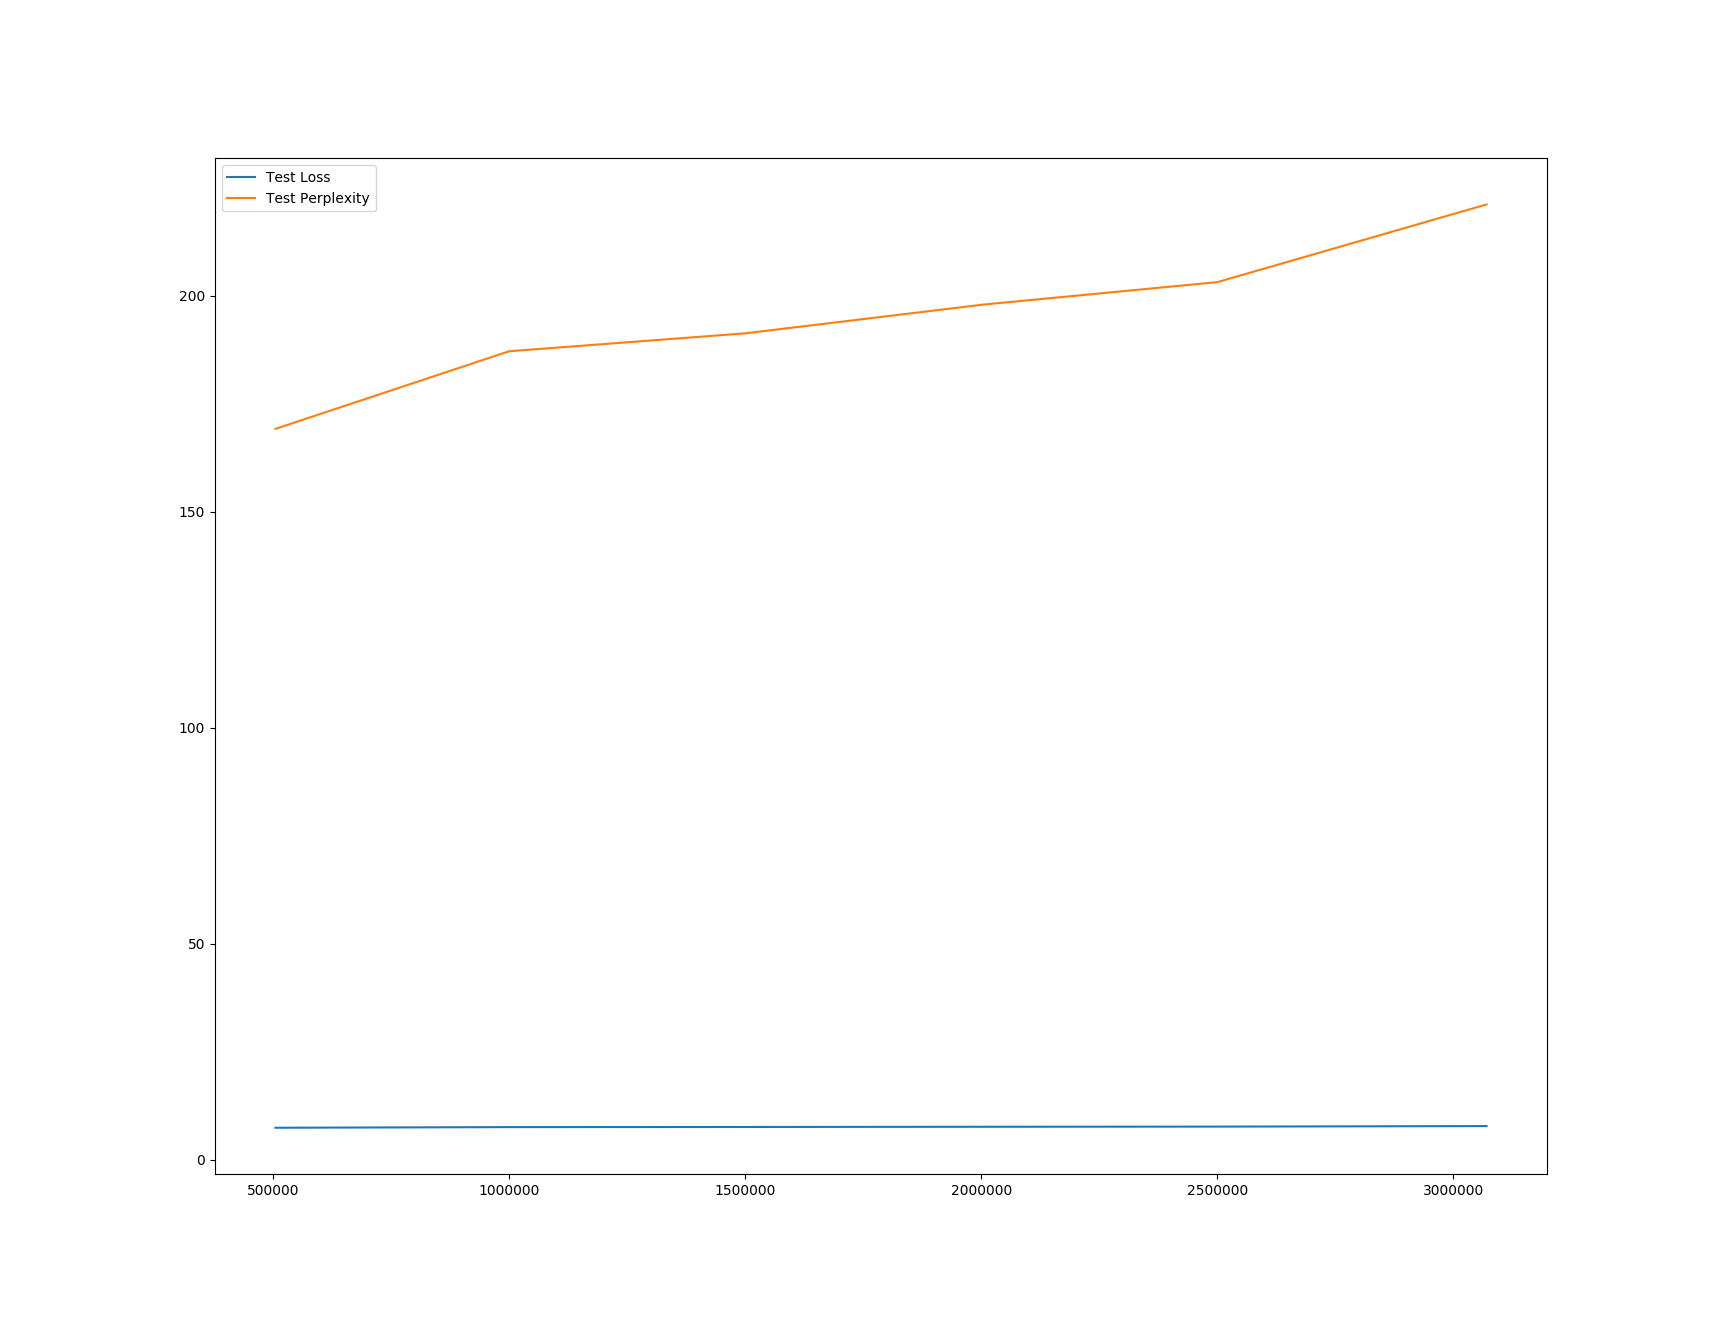
\includegraphics[width=\linewidth]{img/plots/reddit/test_metrics_both.png}
	\centering
	\small
	\text{The loss and perplexity.}
	\endminipage\hfill
	\minipage{0.5\textwidth}
	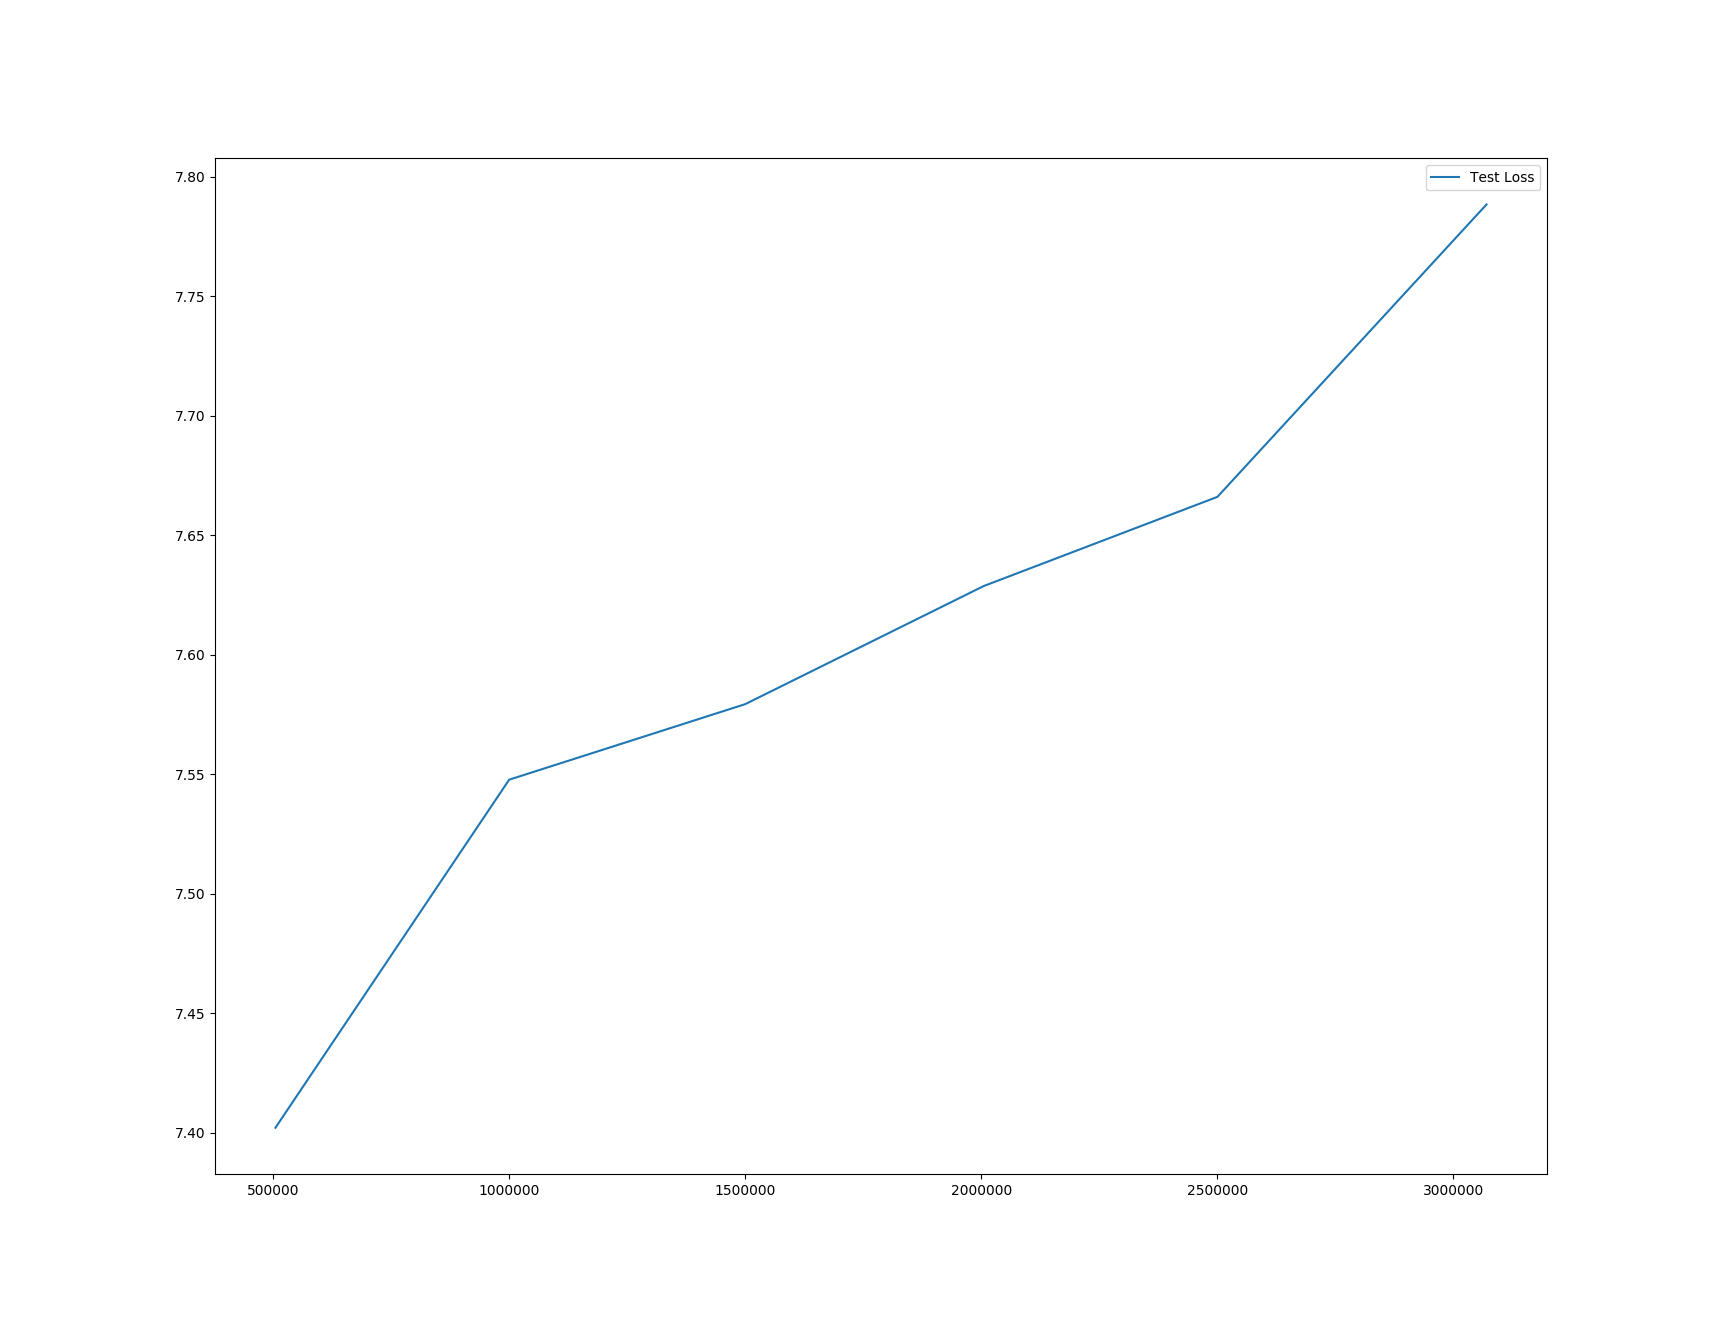
\includegraphics[width=\linewidth]{img/plots/reddit/test_metrics_loss.png}
	\centering
	\small
	\text{Only the loss.}
	\endminipage\hfill
	\caption{The loss and perplexity when evaluating the six different snapshots with the test dataset using the Reddit model.}
	\label{result:test_performance:reddit}
\end{figure}\todo{text unter den Bilderm könnten wir auch nur "loss and perplexity" und "loss" schreibe. Ich überlege gerade ob es diese Bilder überhaupt braucht und wenn ja, ob wir eine Grafik für beide Modelle pro Metrik machen wollen? Die Grafiken wirken jetzt etwas leer.}

\todo{fix scaling of axis}

\paragraph{Is Progress Achieved?} As the results of evaluating the models on the test dataset has shown, it seems that the models achieve an meaningful progress during the training. Even worse, it appears like the models have become poorer over the course of the training. For this reason, we decided that we would like to evaluate the model manually and find out if the generated responses improve when using the six snapshots of the models. We have chosen four different input utterances, two for each model, and generated responses for each of the snapshots. The results can be seen in the Table~\ref{results:example_output:opensubtitles} for the OpenSubtitles model and Table~\ref{results:example_output:reddit} for the Reddit model.

\begin{table}[H]
	\centering
	\begin{adjustbox}{max width=\textwidth}
		\begin{tabular}{ll}
			\toprule
			Input: 	& \texttt{Do you like Joffrey from game of thrones?}\\
			\midrule
			0.5M: 	& \texttt{i m not sure if you re a fan of the movie ,}\\
			& \texttt{but i m not sure if you re a fan of the movie .}\\
			1.0M: 	& \texttt{i m not a fan of the game , but i m not sure if it s a game or not .}\\
			1.5M:	& \texttt{i do nt know what i m talking about .}\\
			2.0M:	& \texttt{i do nt }\\
			2.5M:	& \texttt{i do nt know what i m talking about .}\\
			3.0M:	& \texttt{i do nt know , i just do nt like him .}\\
			\midrule
			Input: 	& \texttt{Which movie can you recommend me?}\\
			\midrule
			0.5M: 	& \texttt{the}\\
			1.0M: 	& \texttt{the movie .}\\
			1.5M:	& \texttt{the one with the}\\
			2.0M:	& \texttt{the dark knight rises}\\
			2.5M:	& \texttt{the prestige}\\
			3.0M:	& \texttt{the movie}\\
			\bottomrule
		\end{tabular}
	\end{adjustbox}
	\caption{Two exemplary dialogs with the Reddit model, one response per snapshot.}
	\label{results:example_output:reddit}
\end{table}
\todo{Format so that all look the same, probably by using tabularx and an X column}

\begin{table}[H]
	\centering
	\begin{adjustbox}{max width=\textwidth}
		\begin{tabular}{ll}
			\toprule
			Input: 	& \texttt{Are you a man or a woman?}\\
			\midrule
			0.5M: 	& \texttt{no , no , no}\\
			1.0M: 	& \texttt{no}\\
			1.5M:	& \texttt{i m not a man}\\
			2.0M:	& \texttt{i m not a woman}\\
			2.5M:	& \texttt{i m a man}\\
			3.0M:	& \texttt{i m not a woman}\\
			\midrule
			Input: 	& \texttt{Why should it not be a good idea to improve you?}\\
			\midrule
			0.5M: 	& \texttt{no}\\
			1.0M: 	& \texttt{i don t know}\\
			1.5M:	& \texttt{because i love you}\\
			2.0M:	& \texttt{because i m a good man}\\
			2.5M:	& \texttt{i m just trying to make a good decision}\\
			3.0M:	& \texttt{i m not a good idea}\\
			\bottomrule
		\end{tabular}
	\end{adjustbox}
	\caption{Two exemplary dialogs with the OpenSubtitles model, one response per snapshot.}
	\label{results:example_output:opensubtitles}
\end{table}

As seen in the examples above, there has indeed been an improvement in the answers, what stands in contradiction to the development of the performance of the models on the test datasets. We suspect from this result, again, that the cross-entropy loss and perplexity are not fit to assess if the responses are meaningful. As we have already described in Chapter~\ref{fundamentals:sent2vec_test}, we were aware of this potential issue; that is why we decided to use an additional metric, namely Sent2Vec embeddings, which we are going to use in the next section.

\paragraph{Sent2Vec Analysis} As described in Chapter~\ref{fundamentals:sent2vec_test}, we leverage Sent2Vec embeddings for measuring the semantic similarity between the generated and expected responses on the test datasets. For this purpose, we have used the pretrained embeddings available on the GitHub page of the project\footnote{https://github.com/epfml/sent2vec}. We decided, that we use both the \emph{Twitter} and \emph{Wikipedia} embeddings for the assessment. The results can be seen in the Figures~\ref{results:sent2vec:opensubtitles:results} and~\ref{results:sent2vec:reddit:results}. It is obvious that both the Reddit and OpenSubtitles models perform better on the pretrained \emph{Wikipedia} embeddings in comparison to the pretrained \emph{Twitter} embeddings. This is probably related to the ``compressed'' language used when writing tweets (e.g. ``w/o'' instead of ``without''). In conclusion, the results of this analysis are dependent on the Sent2Vec embeddings, as expected. However, both results are poor, with the results from the Reddit model being about twice as good as results from the OpenSubtitles model (see Tables~\ref{results:sent2vec:opensubtitles:results_table} and~\ref{results:sent2vec:reddit:results_table}). The OpenSubtitles model starts with an average similarity of $0.167$ for the first snapshot and rises up to $0.204$ for the last snapshot. The Reddit model starts with an average value of $0.336$ for the first snapshot and increases to $0.359$ for the last snapshot. This means that the responses of the Reddit model match the expected responses much better from a semantic perspective as the responses of the OpenSubtitles model do. \todo{The Reasen for this eye-catching difference is perhaps due to the difference between spoken language and written language?}In summary, the results of both models are unsatisfactory, as the maximum achievable similarity is $1.0$.

\begin{figure}[H]
	\minipage{0.5\textwidth}
	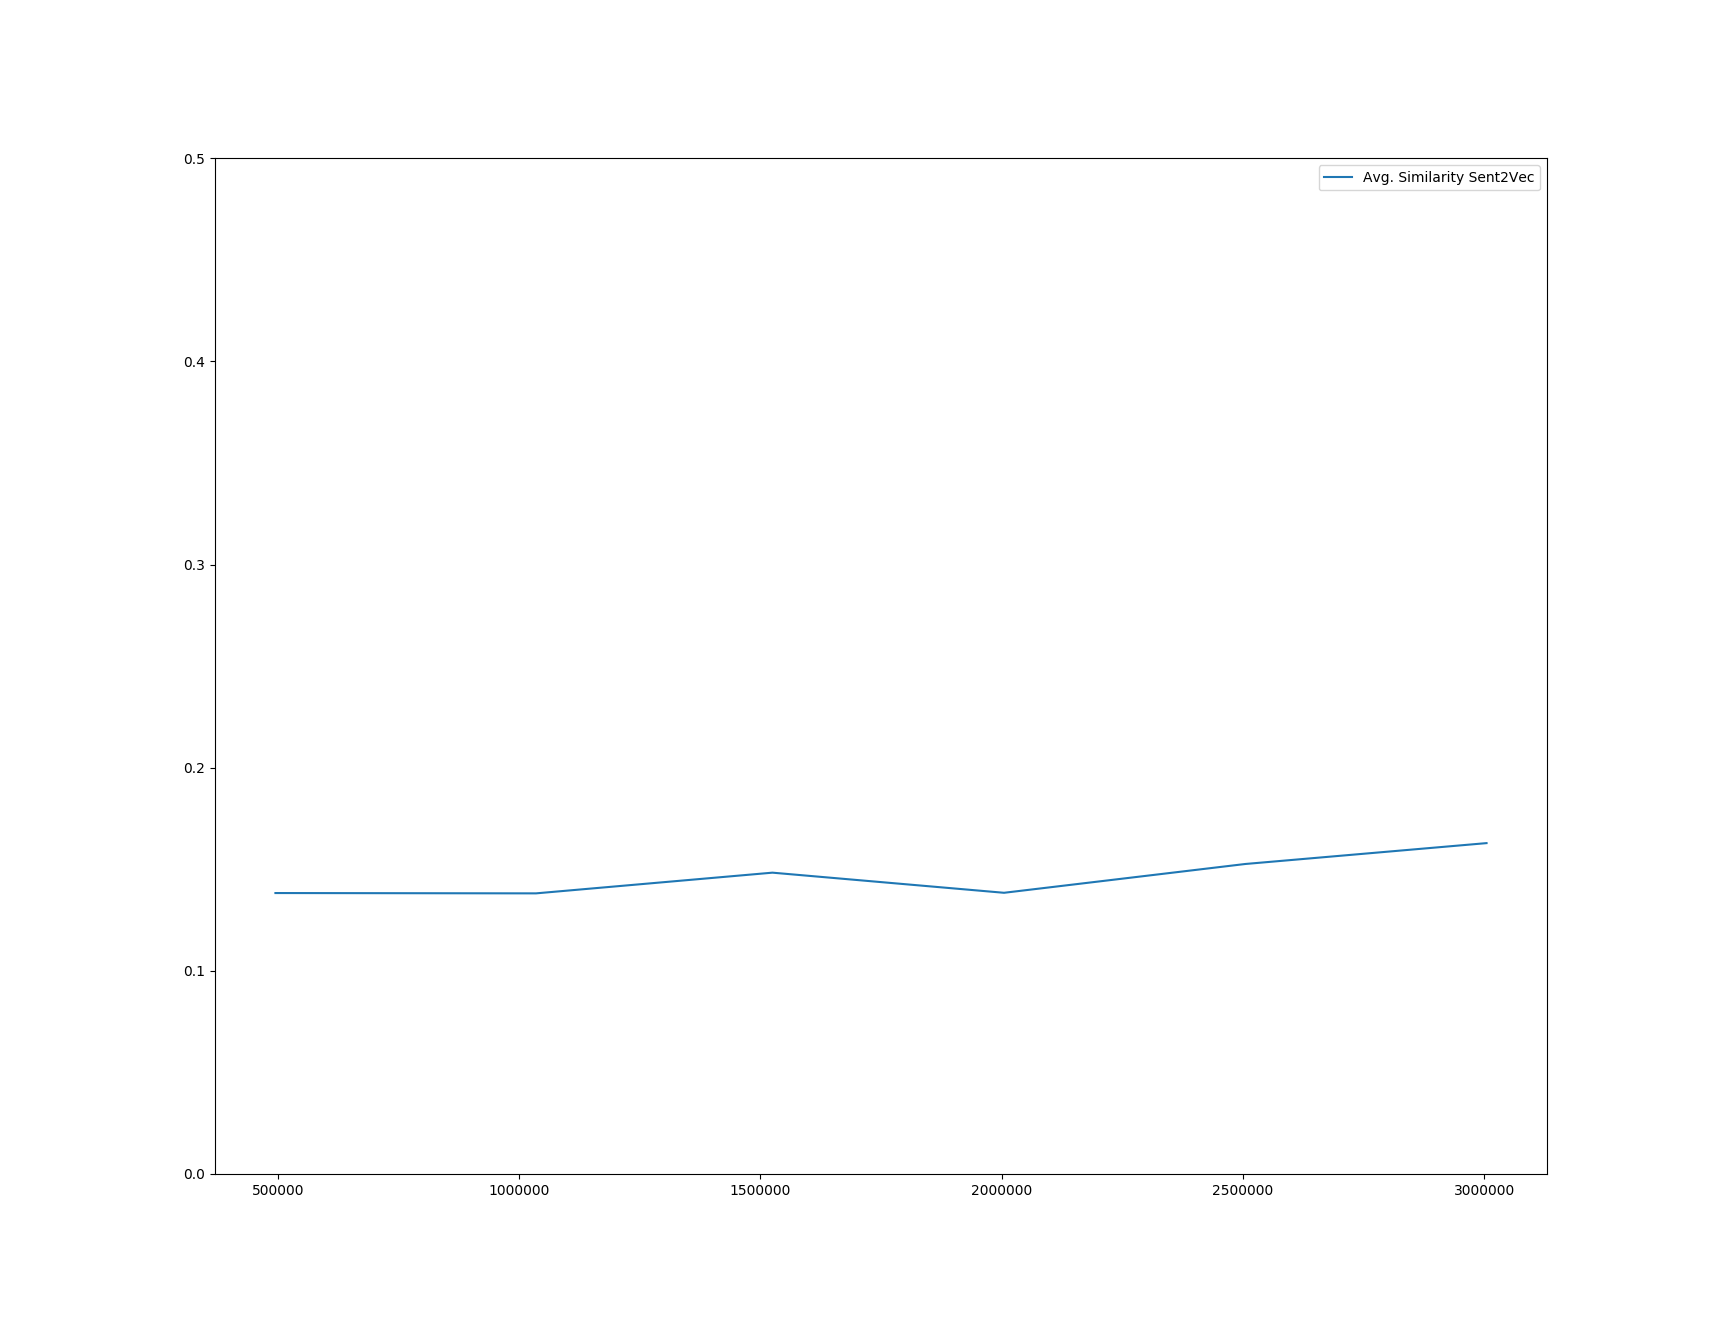
\includegraphics[width=\linewidth]{img/plots/opensubtitles_not_reversed/s2v_wiki_cosine_similarity.png}
	\centering
	\small
	\text{\emph{Wikipedia}}
	\endminipage\hfill
	\minipage{0.5\textwidth}
	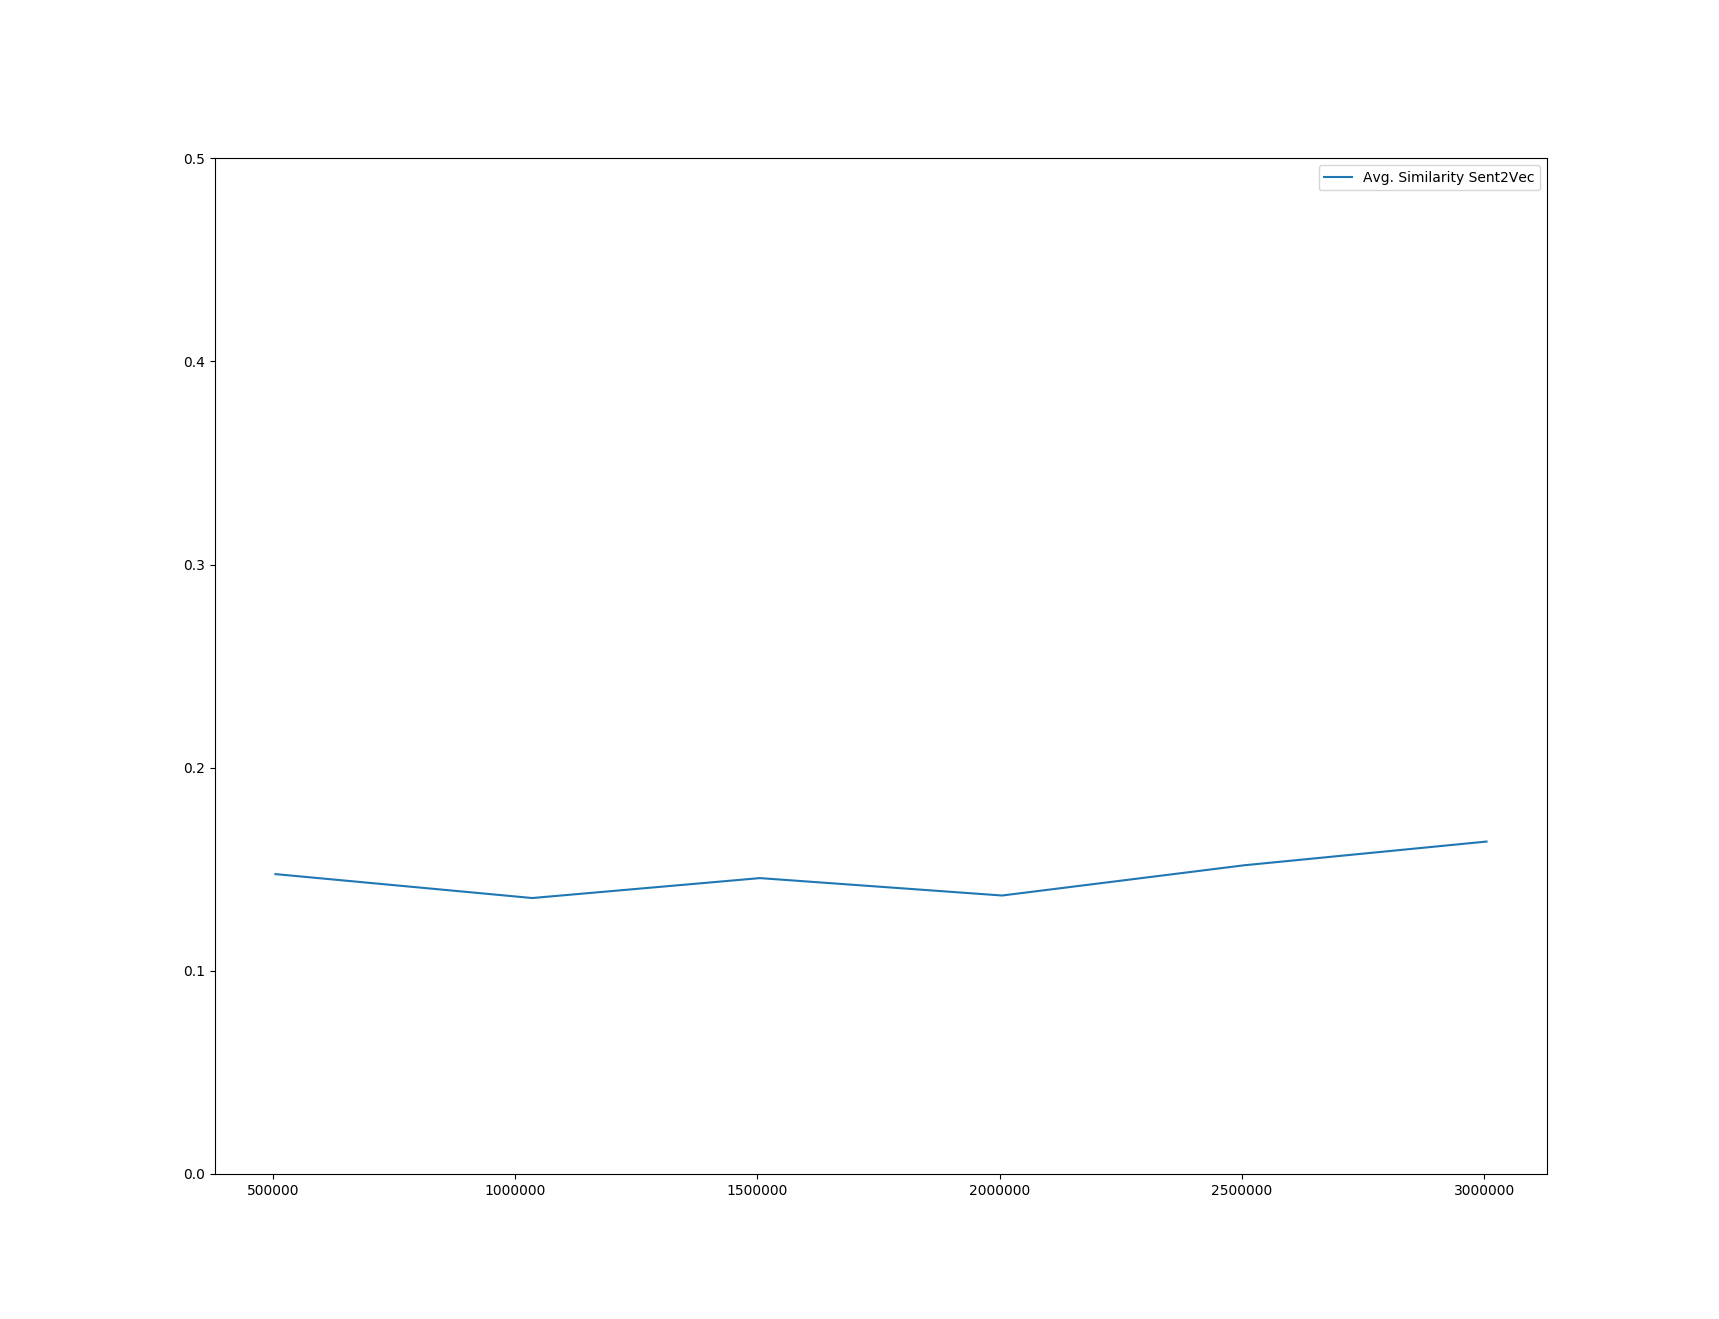
\includegraphics[width=\linewidth]{img/plots/opensubtitles_not_reversed/s2v_twitter_cosine_similarity.png}
	\centering
	\small
	\text{\emph{Twitter}}
	\endminipage\hfill
	\caption{Results of the evaluation with Sent2Vec on the outputs of the OpenSubtitles model when using the test dataset. The ticks on the x-axis show the different snapshots and the y-axis the average semantic similarity for each snapshot.}
	\label{results:sent2vec:opensubtitles:results}
\end{figure}

\begin{table}[H]
	\centering
	\begin{adjustbox}{max width=\textwidth}
		\begin{tabular}{lcc}
			\toprule
			Snapshot & Avg. Similarity (\emph{Wikipedia}) & Avg. Similarity (\emph{Twitter})\\
			\midrule
			0.5M & $0.16749$ & $0.13827$\\
			1.0M & $0.19111$ & $0.13811$\\
			1.5M & $0.19418$ & $0.14831$\\
			2.0M & $0.19176$ & $0.13840$\\
			2.5M & $0.20118$ & $0.15258$\\
			3.0M & $0.20452$ & $0.16285$\\
			\bottomrule
		\end{tabular}
	\end{adjustbox}
	\caption{The average similarities when using the Sent2Vec metric on the expected and generated responses from the OpenSubtitles model per snapshot.}
	\label{results:sent2vec:opensubtitles:results_table}
\end{table}

\begin{figure}[H]
	\minipage{0.5\textwidth}
	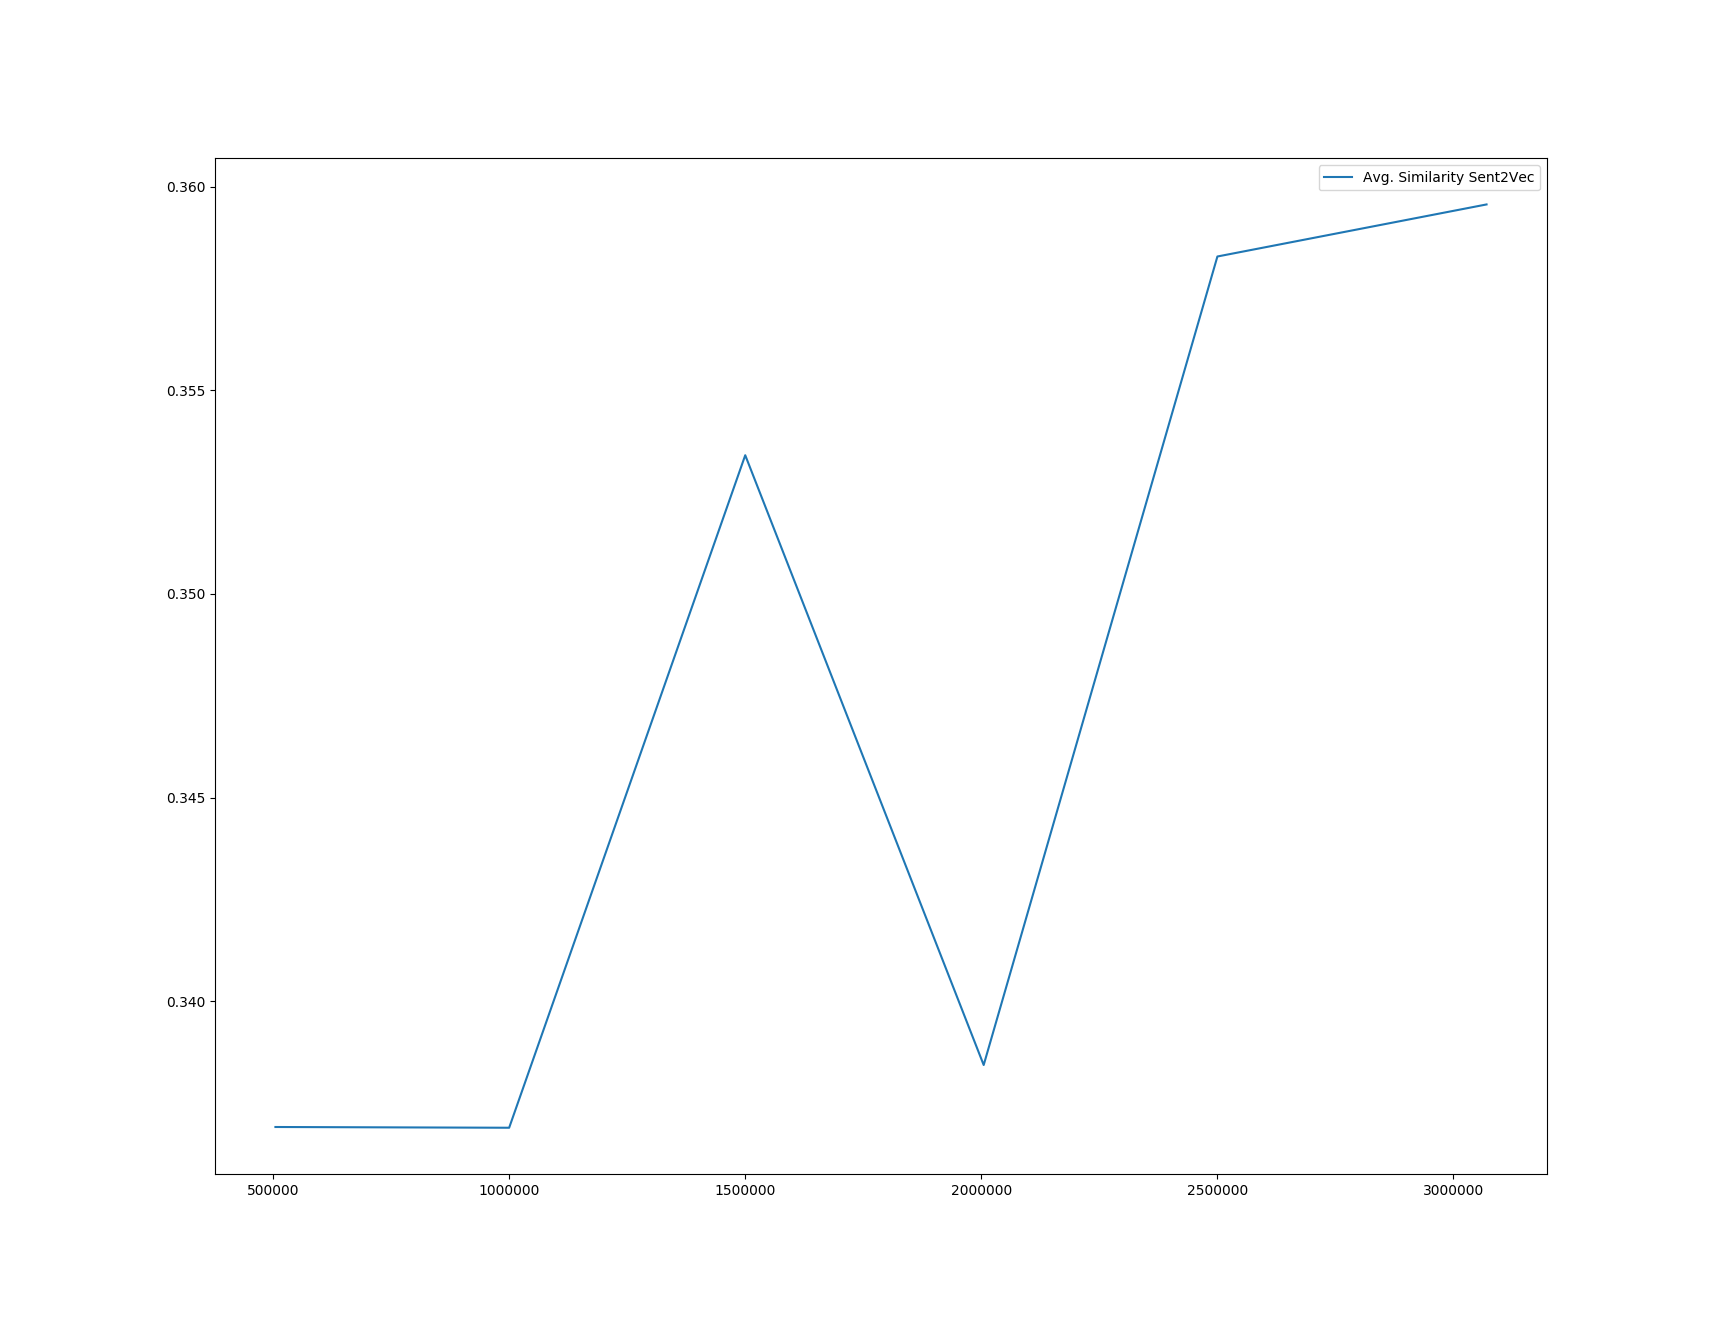
\includegraphics[width=\linewidth]{img/plots/reddit/s2v_wiki_cosine_similarity.png}
	\centering
	\small
	\text{\emph{Wikipedia}}
	\endminipage\hfill
	\minipage{0.5\textwidth}
	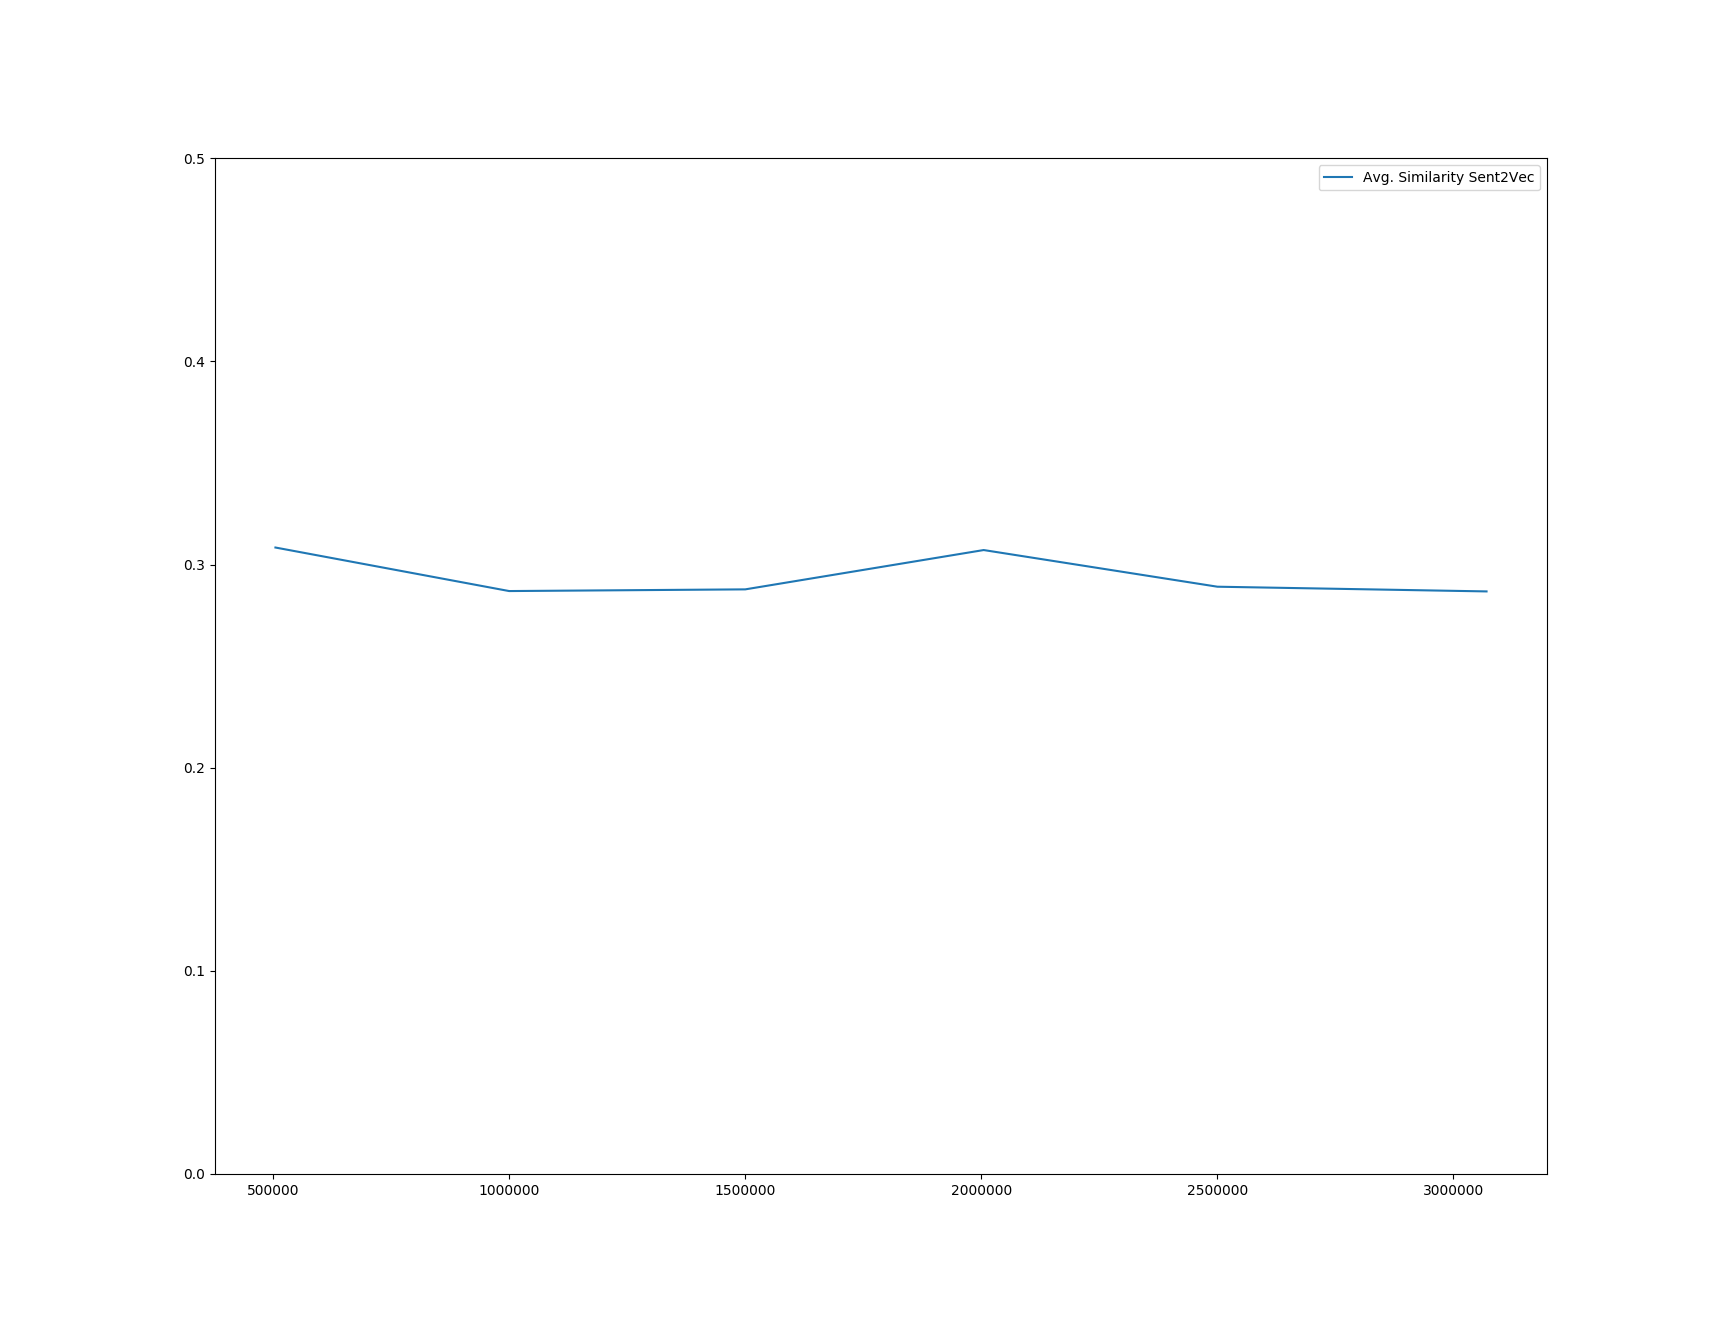
\includegraphics[width=\linewidth]{img/plots/reddit/s2v_twitter_cosine_similarity.png}
	\centering
	\small
	\text{\emph{Twitter}}
	\endminipage\hfill
	\caption{Results of the evaluation with Sent2Vec on the outputs of the Reddit model when using the test dataset. The ticks on the x-axis show the different snapshots and the y-axis the average semantic similarity for each snapshot.}
	\label{results:sent2vec:reddit:results}
\end{figure}
\begin{table}[H]
	\centering
	\begin{adjustbox}{max width=\textwidth}
		\begin{tabular}{lcc}
			\toprule
			Snapshot & Avg. Similarity (\emph{Wikipedia}) & Avg. Similarity (\emph{Twitter})\\
			\midrule
			0.5M & $0.33691$ & $0.30837$\\
			1.0M & $0.33689$ & $0.28694$\\
			1.5M & $0.35340$ & $0.28777$\\
			2.0M & $0.33843$ & $0.30713$\\
			2.5M & $0.35828$ & $0.28908$\\
			3.0M & $0.35956$ & $0.28676$\\
			\bottomrule
		\end{tabular}
	\end{adjustbox}
	\caption{The average similarities when using the Sent2Vec metric on the expected and generated responses from the Reddit model per snapshot.}
	\label{results:sent2vec:reddit:results_table}
\end{table}

\paragraph{Generic Response are a Problem} A potential reason for the poor results when using the Sent2Vec metric could be based on our observation that both models often generate generic responses (e.g. ``i don t know'', ``i m not sure what you re saying''). Our first idea to analyze this is to see what kind of sentences the models produce with the inputs of the test datasets. We did an analysis on the generated responses and quickly noticed that there are a few sentences, which are often predicted by the models (see Tables~\ref{results:test_performance:opensubtitles_sample_outputs} and~\ref{results:test_performance:reddit_sample_outputs}). As one can see in the column \emph{Percentage}, these generic responses take up a great share of all the generated responses. The top 10 responses from the OpenSubtitles model make up 45.77\% of all outputs, where the same for the Reddit only sums up to 33.02\% of all outputs.
\\
\begin{table}[H]
	\centering
	\begin{adjustbox}{max width=\textwidth}
		\begin{tabular}{lcc}
			\toprule
			Sentence & Occurrence Frequency & Percentage \\ \midrule
			\texttt{i m not gon na let you go} & 41853 & 16.74\%\\
			\texttt{i m not sure i can trust you} & 21263 & 8.51\%\\
			\texttt{i m not gon na say anything} & 9163 & 3.67\%\\
			\texttt{i m not gon na let that happen} & 7426 & 2.97\%\\
			\texttt{i m sorry} & 7235 & 2.89\\
			\texttt{you re not gon na believe this} & 7068 & 2.83\%\\
			\texttt{you re not gon na believe me} & 6878 & 2.75\%\\
			\texttt{i m not gon na hurt} you & 4829 & 1.93\%\\
			\texttt{i m not a fan} & 4468 & 1.79\%\\
			\texttt{i m not sure} & 4215 & 1.69\%\\
			\midrule
			Summed up & 114408 & 45.77\%\\
			\midrule
			\midrule
			Total Sentences Count & 249984 & 100.00\%\\
			\bottomrule
		\end{tabular}
	\end{adjustbox}
	\caption{Top 10 most generated responses with respective occurrence frequencies when using the last OpenSubtitles snapshot and the test dataset.}
	\label{results:test_performance:opensubtitles_sample_outputs}
\end{table}\todo{make tables the same width!}

\begin{table}[H]
	\centering
	\begin{adjustbox}{max width=\textwidth}
		\begin{tabular}{lcc}
			\toprule
			Sentence & Occurrence Frequency & Percentage\\ \midrule
			\texttt{i m not sure if i m being sarcastic or not .} & 17486 & 7.00\%\\
			\texttt{i think it s a bit of a stretch .} & 13058 & 5.22\%\\
			\texttt{i m not sure if you re being sarcastic or not .} & 11647 & 4.66\%\\
			\texttt{i m not sure if i m a <unknown> or not .} & 8307 & 3.32\%\\
			\texttt{i m not sure if you re joking or not .} & 7932 & 3.17\%\\
			\texttt{i was thinking the same thing .} & 7579 & 3.03\%\\
			\texttt{<unknown>} & 6210 & 2.48\%\\
			\texttt{i m not sure if i m going to watch this or not .} & 4257 & 1.70\%\\
			\specialcell{\texttt{i m not sure if i m a fan of the show , but i m}\\\texttt{pretty sure that s a <unknown> .}} & 3232 & 1.29\%\\
			\texttt{i m not sure if i m going to watch it or not .} & 3079 & 1.23\%\\
			\midrule
			Summed up & 82797 & 33.02\%\\
			\midrule
			\midrule
			Total Amount Sentences & 249984 & 100.00\%\\
			\bottomrule
		\end{tabular}
	\end{adjustbox}
	\caption{Top 10 most generated sentences with respective occurrence frequencies when using the last Reddit snapshot and the test dataset.}
	\label{results:test_performance:reddit_sample_outputs}
\end{table}\todo{make tables the same width!}

\paragraph{Does Filtering of Generic Responses Help?} As seen in the both tables above, there are certain responses which are generated a lot of time and are pretty generic and meaningless in most contexts. Because of that, we think it would be a good idea to evaluate the models under the Sent2Vec metric one more time, but this time with the top $n$ most generated responses filtered out. We do this expecting that the generic sentences are the cause of the small average similarities. The results of the analysis with the top $n$ most generated responses filtered out is shown in Table~\ref{results:sent2vec:opensubtitles:top_n_results_table} and~\ref{results:sent2vec:reddit:top_n_results_table}. For this analysis, we only use the \emph{Wikipedia} embeddings as it has shown a better performance for both of our models before.
\\
\begin{table}[H]
	\centering
	\begin{adjustbox}{max width=\textwidth}
		\begin{tabular}{lccc}
			\toprule
			Snapshot & $n = 1$ & $n = 5$ & $n = 10$\\
			\midrule
			0.5M & $0.16679$ & $0.16804$ & $0.16854$\\
			1.0M & $0.19329$ & $0.19394$ & $0.19575$\\
			1.5M & $0.19491$ & $0.19519$ & $0.19539$\\
			2.0M & $0.19215$ & $0.19192$ & $0.19284$\\
			2.5M & $0.20102$ & $0.20127$ & $0.20182$\\
			3.0M & $0.20431$ & $0.20547$ & $0.20568$\\
			\bottomrule
		\end{tabular}
	\end{adjustbox}
	\caption{The average similarities when applying the Sent2Vec metric on the expected and generated responses on the test dataset when filtering out the top $n$ most generated responses for the OpenSubtitles model.}
	\label{results:sent2vec:opensubtitles:top_n_results_table}
\end{table}

\begin{table}[H]
	\centering
	\begin{adjustbox}{max width=\textwidth}
		\begin{tabular}{lccc}
			\toprule
			Snapshot & $n = 1$ & $n = 5$ & $n = 10$\\
			\midrule
			0.5M & $0.33772$ & $0.34101$ & $0.34589$\\
			1.0M & $0.34225$ & $0.34238$ & $0.34295$\\
			1.5M & $0.35383$ & $0.35605$ & $0.35564$\\
			2.0M & $0.34008$ & $0.34009$ & $0.34198$\\
			2.5M & $0.35937$ & $0.36142$ & $0.36175$\\
			3.0M & $0.36043$ & $0.35950$ & $0.36313$\\
			\bottomrule
		\end{tabular}
	\end{adjustbox}
	\caption{The average similarities when applying the Sent2Vec metric on the expected and generated responses on the test dataset when filtering out the top $n$ most generated responses for the Reddit model.}
	\label{results:sent2vec:reddit:top_n_results_table}
\end{table}

As seen above, the filtering of the most used responses does not help significantly when it comes to the Sent2Vec evaluation. We currently cannot say if this problem is just apparent in our specific use-case or inherent to the metric itself. To come to a definitive conclusion, we would have to investigate further by using this metric for evaluating other models.

\paragraph{Mixed Feelings about Performance Metrics} As seen in this chapter, the performance metrics we use to evaluate the models tell us an indifferent story about the resulting models. On one hand, we see that the training performed acceptable and the learning process ran as expected. However, as we subsequently test these trained models against the test datasets with the different metrics, it looks like the performance decreased over the duration of the training. Our subjective opinion could not confirm this after we were ``talking'' to both models for an extensive period of time. We think the biggest problem for the evaluation is the large portion of generic responses both models seem to generate. To identify the cause of this generic responses, we will now analyze the language model which both models have learned while training, trying to establish a connection between the language model in the datasets and the ones produced by the models.

\section{Development of Language Model}
\label{results:development_language_model}
In this chapter we are investigating into the language models produced by the trained and try to identify a reason for the generic responses.

\subsection{Uni- and Bi-gram Distributions over Time}
Initially, we are comparing to compare the uni- and bi-gram distributions of the training datasets with the distributions produced when evaluating the models with the test datasets. For this purpose we have generated unigram and bigram statistics using \texttt{nltk} on the training datasets and outputs generated by the models.

\paragraph{OpenSubtitles} The OpenSubtitles has the most evenly spread distribution (see Figure~\ref{results:bigram:distributions:opensubtitles}) when using the first snapshot (i.e. 0.5M). We observe a pattern when we look at all distributions of the OpenSubtitles model. At the beginning, it starts with a rather evenly spread distribution of uni- and bi-grams. As the training proceeds, these distributions shift to a more right-leaned when looking at the distributions for the snapshot 1.0M. The distributions then return to be more evenly distributed again. This pattern repeats until the last snapshot, with one being evenly distributed whereas the next is then again more right-leaned.

We cannot provide a complete explanation for this behavior, but we assume that this is related to the rather noisey dataset we are using for the OpenSubtitles model. This probably leads to the model being confused, rejecting what it has already learned and trying to fit to the newly provided samples. Because of the fact that we cannot fully explain this behavior, we are going to analyze the development of the diversity of the uni-/bi-gram and sentences over the course of the training.

The behavior of the uni-gram distributions develops in a similar way, therefore we documented these visualizations in the Appendix~\ref{appendix:unigram_distributions}.

\begin{figure}[H]
	\minipage{0.5\textwidth}
	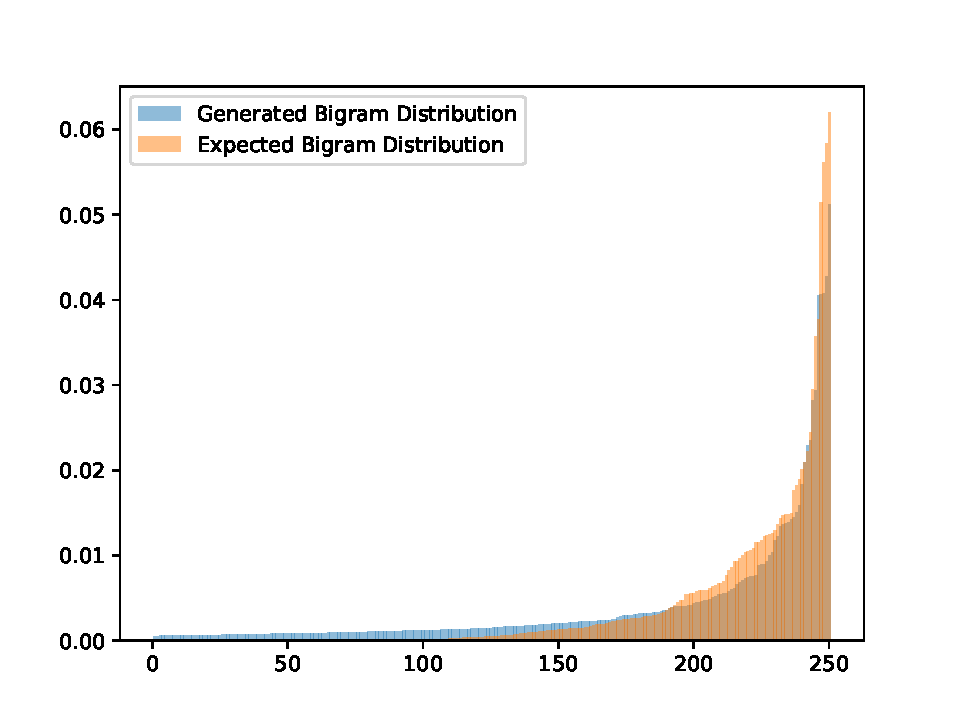
\includegraphics[width=\linewidth]{img/plots/opensubtitles_not_reversed/bigram_distribution_comparison_step_500000.pdf}
	\centering
	\small
	\text{Snapshot 0.5M}
	\endminipage\hfill
	\minipage{0.5\textwidth}
	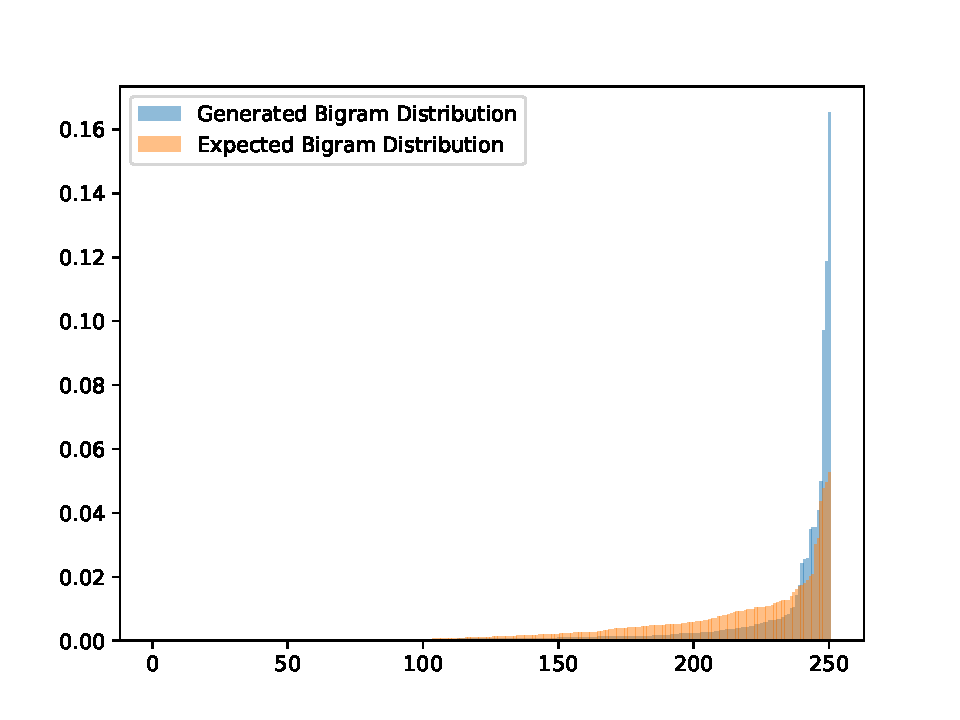
\includegraphics[width=\linewidth]{img/plots/opensubtitles_not_reversed/bigram_distribution_comparison_step_1000000.pdf}
	\centering
	\small
	\text{Snapshot 1.0M}
	\endminipage\hfill
	\minipage{0.5\textwidth}
	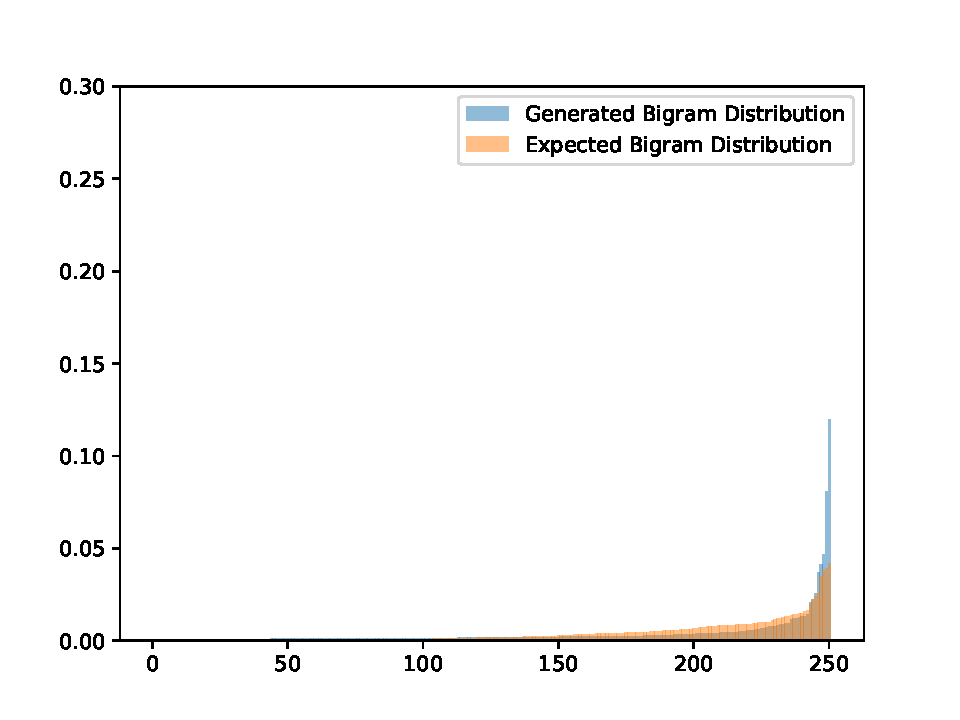
\includegraphics[width=\linewidth]{img/plots/opensubtitles_not_reversed/bigram_distribution_comparison_step_1500000.pdf}
	\centering
	\small
	\text{Snapshot 1.5M}
	\endminipage\hfill
	\minipage{0.5\textwidth}
	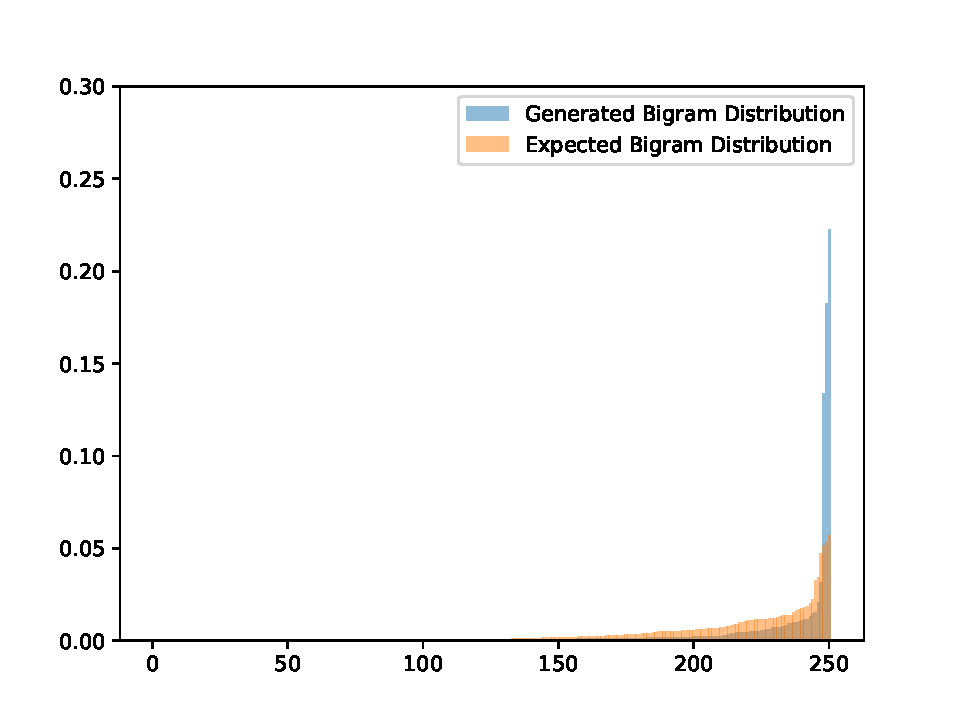
\includegraphics[width=\linewidth]{img/plots/opensubtitles_not_reversed/bigram_distribution_comparison_step_2000000.pdf}
	\centering
	\small
	\text{Snapshot 2.0M}
	\endminipage\hfill
	\minipage{0.5\textwidth}
	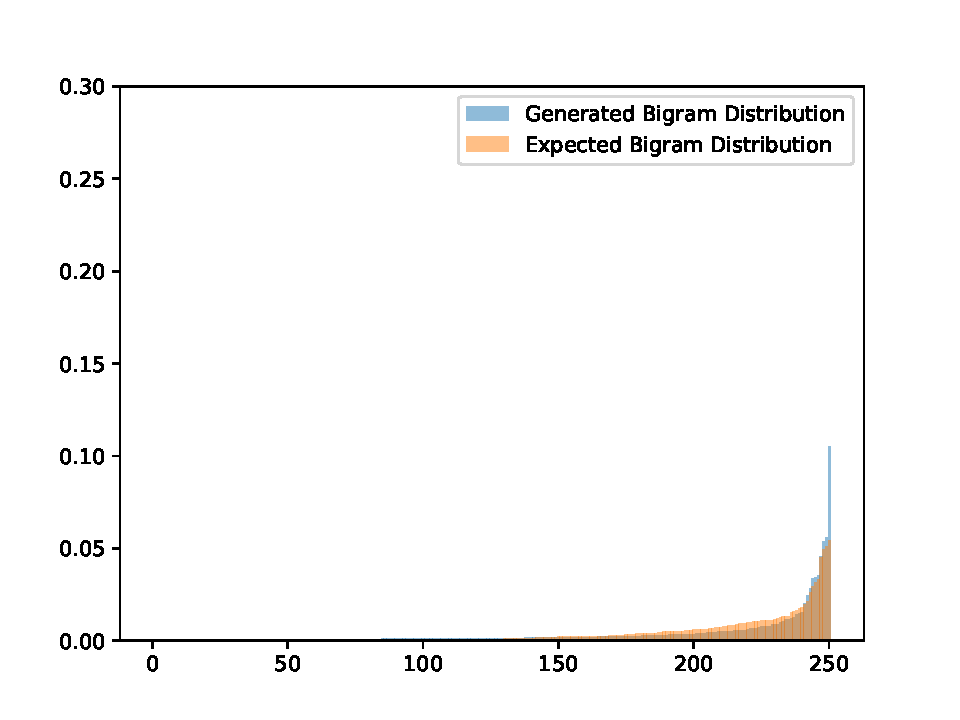
\includegraphics[width=\linewidth]{img/plots/opensubtitles_not_reversed/bigram_distribution_comparison_step_2500000.pdf}
	\centering
	\small
	\text{Snapshot 2.5M}
	\endminipage\hfill
	\minipage{0.5\textwidth}
	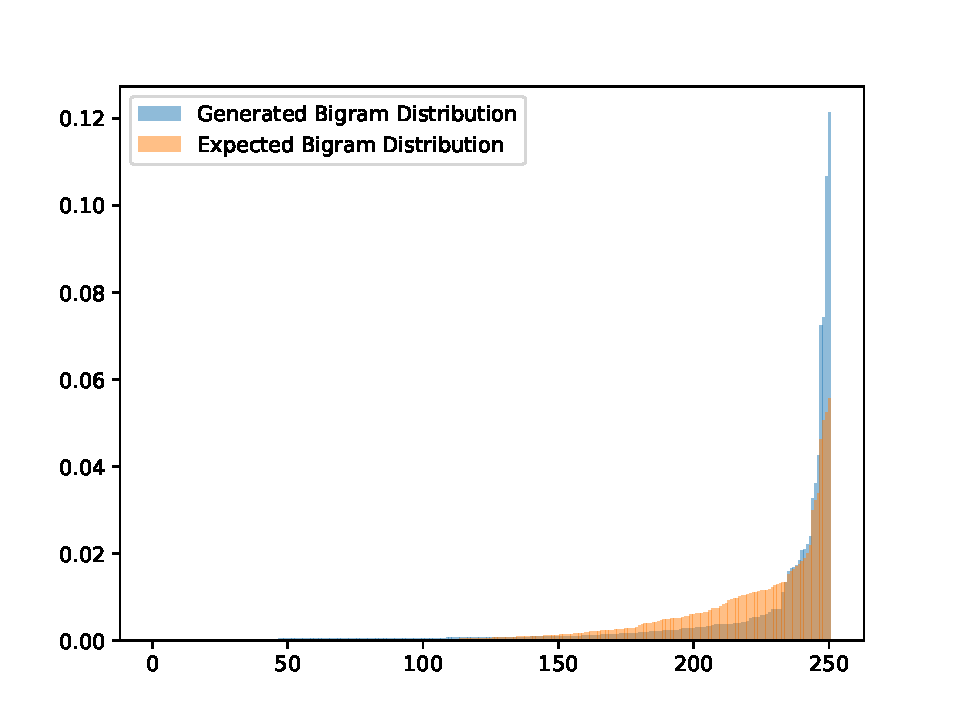
\includegraphics[width=\linewidth]{img/plots/opensubtitles_not_reversed/bigram_distribution_comparison_step_3000000.pdf}
	\centering
	\small
	\text{Snapshot 3.0M}
	\endminipage\hfill
	\caption{Comparison of the distributions of the top 250 most used bi-grams for the responses of the OpenSubtitles model (orange) when using the test dataset and the distribution within the training dataset (blue). The distributions are compared for each snapshot available.}
	\label{results:bigram:distributions:opensubtitles}
\end{figure}

\paragraph{Reddit} The distributions for the Reddit model reveal an interesting development (see Figure~\ref{results:bigram:distributions:reddit}). In the beginning, same as with the OpenSubtitles, the distributions are evenly spread. However, as the training continues, the distributions increasingly better fit the expected distributions, until the fit reaches the highest overlap when using the 1.5M and 2.0M snapshots. From this point onwards, the distributions start to drift apart again. This coincides in our opinion, that the Reddit model is at its performance peak when using the snapshot 2.0M. This is probably associated with the fact that we are doing more than two epochs over the full dataset. From the snapshot 2.0M on, the model itself starts to become worse, as the diversity and quality of the responses starts to decline. We are going to analyze this assumption below.

The behavior of the uni-gram distributions develops in a similar way, therefore we documented these visualizations in the Appendix~\ref{appendix:unigram_distributions}.

\begin{figure}[H]
	\minipage{0.5\textwidth}
	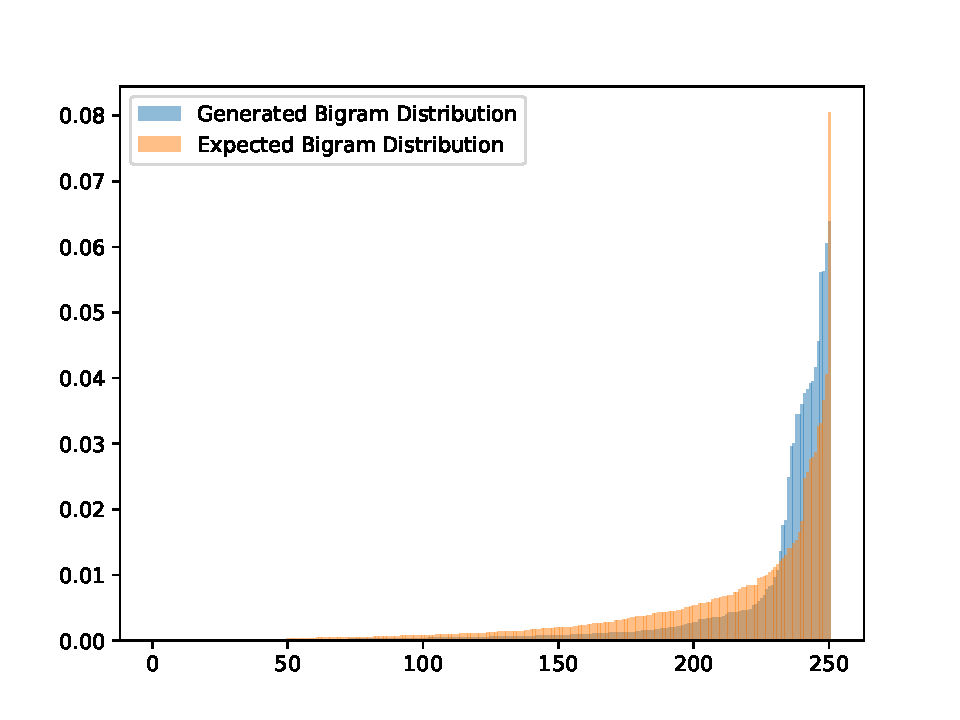
\includegraphics[width=\linewidth]{img/plots/reddit/bigram_distribution_comparison_step_500000.pdf}
	\centering
	\small
	\text{Snapshot 0.5M}
	\endminipage\hfill
	\minipage{0.5\textwidth}
	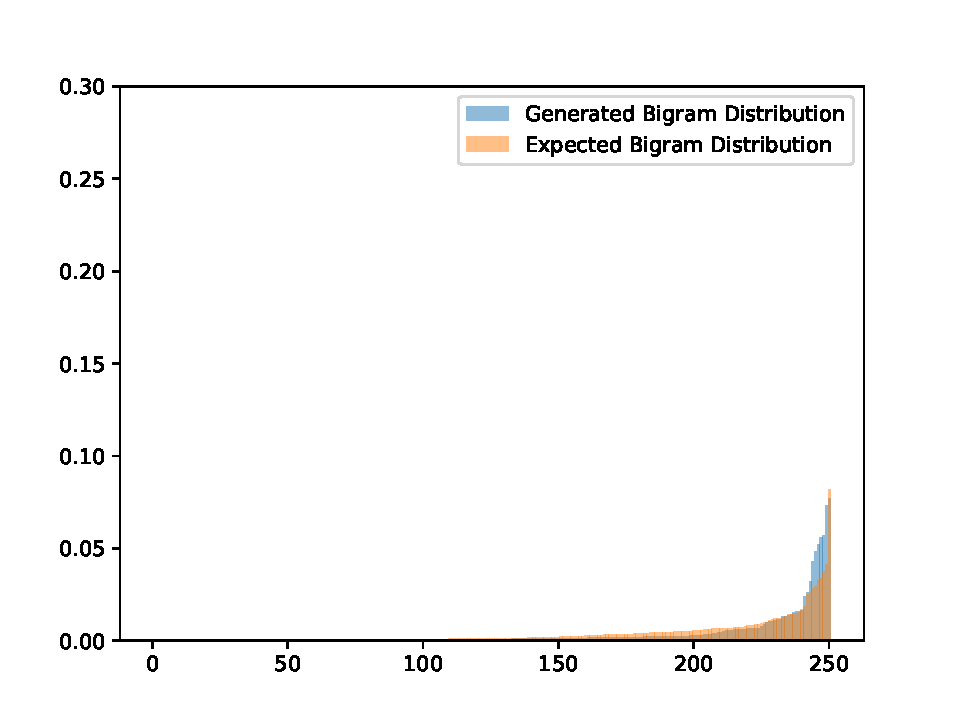
\includegraphics[width=\linewidth]{img/plots/reddit/bigram_distribution_comparison_step_1000000.pdf}
	\centering
	\small
	\text{Snapshot 1.0M}
	\endminipage\hfill
	\minipage{0.5\textwidth}
	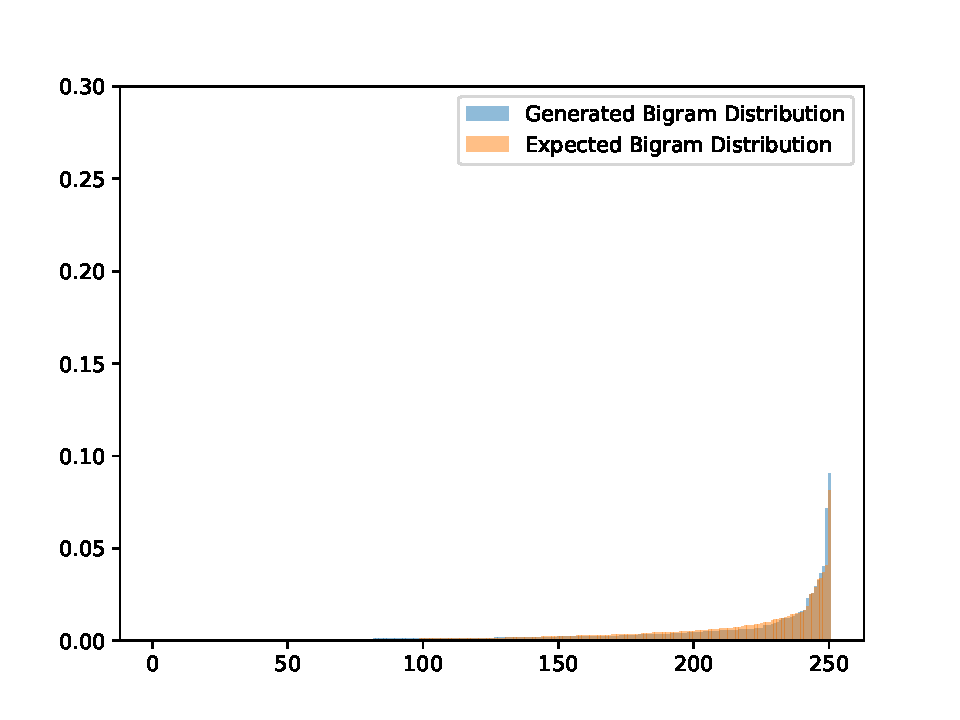
\includegraphics[width=\linewidth]{img/plots/reddit/bigram_distribution_comparison_step_1500000.pdf}
	\centering
	\small
	\text{Snapshot 1.5M}
	\endminipage\hfill
	\minipage{0.5\textwidth}
	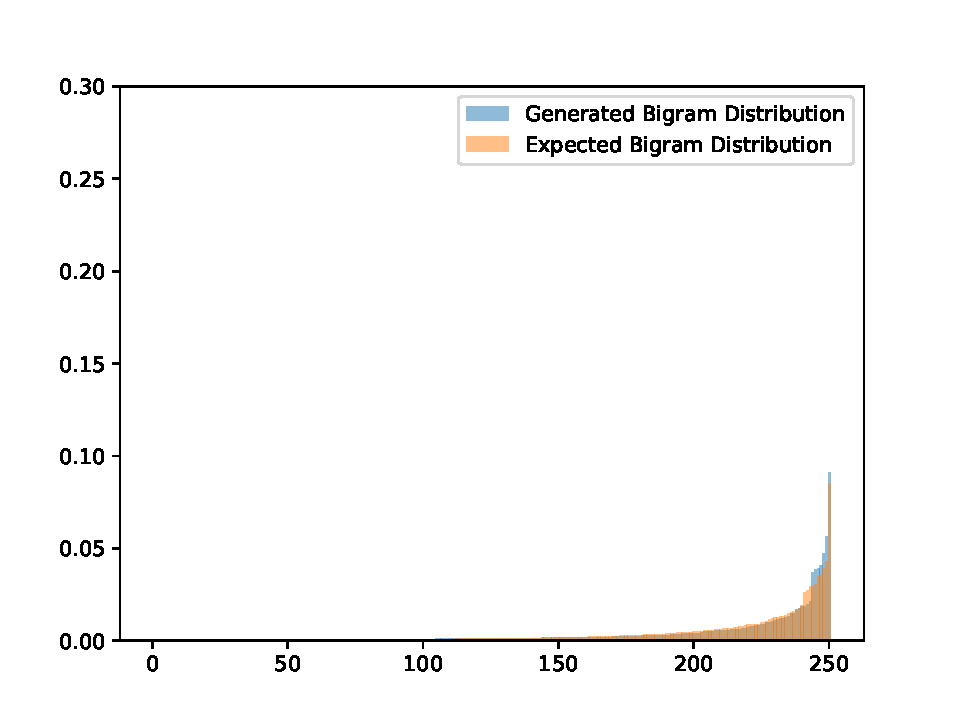
\includegraphics[width=\linewidth]{img/plots/reddit/bigram_distribution_comparison_step_2000000.pdf}
	\centering
	\small
	\text{Snapshot 2.0M}
	\endminipage\hfill
	\minipage{0.5\textwidth}
	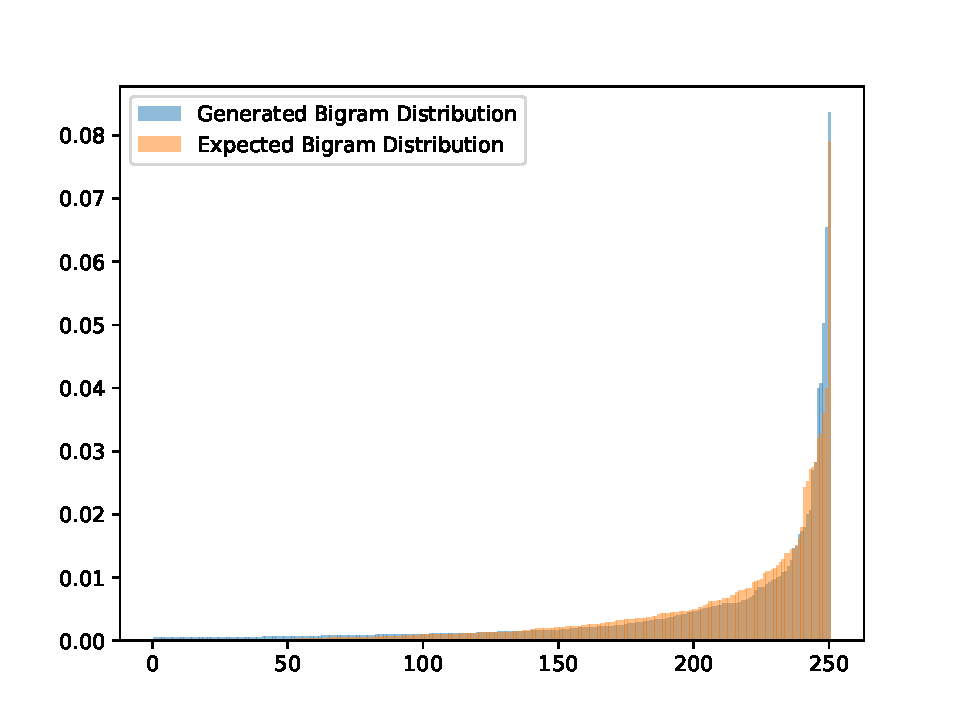
\includegraphics[width=\linewidth]{img/plots/reddit/bigram_distribution_comparison_step_2500000.pdf}
	\centering
	\small
	\text{Snapshot 2.5M}
	\endminipage\hfill
	\minipage{0.5\textwidth}
	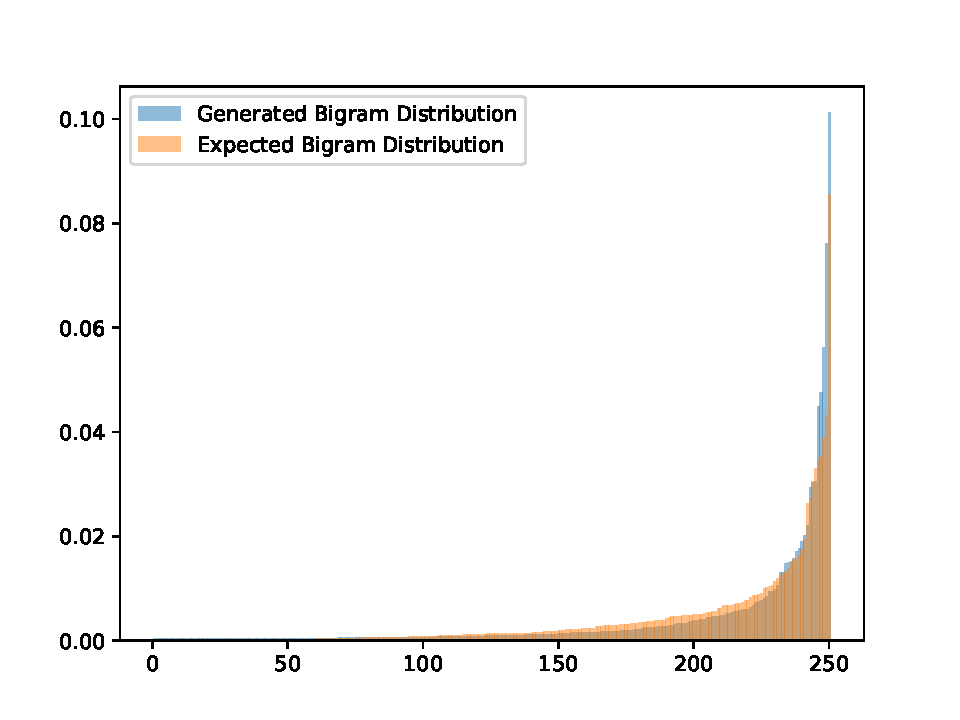
\includegraphics[width=\linewidth]{img/plots/reddit/bigram_distribution_comparison_step_3000000.pdf}
	\centering
	\small
	\text{Snapshot 3.0M}
	\endminipage\hfill
	\caption{Comparison of the distributions of the top 250 most used bi-grams for the responses of the Reddit model (orange) when using the test dataset and the distribution within the training dataset (blue). The distributions are compared for each snapshot available.}
	\label{results:bigram:distributions:reddit}
\end{figure}

\subsection{Language Diversity}
We now analyze the language diversity of the outputs produced by the two models over the different snapshots.  For this purpose, we are analyzing how large the share of the top 10 uni-, bi-gram and sentences within the entirety of the generated responses is when using the respective test datasets. The results can be seen in the Table~\ref{results:top_10_frequency:reddit} for Reddit and \ref{results:top_10_frequency:OpenSubtitles} for OpenSubtitles. 

In the Tables, three different categories are shown: Uni-grams, bi-grams and sentences. For each of these categories, we have summed up the occurrence frequencies of the top 10 most occurring instances for the respective category. These sums can be seen in the \emph{Top Count} columns. The columns named \emph{All Count} contain the total amount of all instances for each category per snapshot. The ratio of the \emph{Top Count} value compared to the \emph{All Count} value can be seen in the \emph{Top Freq.} column for each category and snapshot.
\todo{add more telling column names to the tables}

The first thing which is noticeable when comparing the values from the two tables is that the Reddit outputs seem to be composed of much more uni- and bi-grams. This can be seen when comparing the \emph{Top Count} values from both tables. This signifies that the outputs of the Reddit model are of greater length on average than the outputs of the OpenSubtitles model because the number of sentences stays the same for both. This might be one of the reasons why the results from the Sent2Vec analysis (see Chapter~\ref{results:performance_on_test_datasets}) are much better for the Reddit than the OpenSubtitles model.

At first, we tried to see a tendency on how language diversity develops when using the absolute values from the \emph{Top Count} columns, but we could not. This is the reason why we added the relative values from the \emph{Top Freq.} columns. The problem with using the absolute values is, that the number used uni- and bi-grams changes between the snapshots. However, when we start using the relative values we can compare the different snapshots to each other by means of diversity of the outputs. 

\begin{table}[H]
	\centering
	\begin{adjustbox}{max width=\textwidth}
		\begin{tabular}{llllllllll}
			\toprule
			& Words &&&Bi-Gramm&&&Sentences&&\\
			Snapshot & Top Count & All Count& Top freq. \%&  Top Count& All Count& Top freq. \%&  Top Count& All Count& Top freq. \%\\
			\midrule
			0.5M & 516,756	 & 1,035,956	& 49.88\%	&306,757	&1,033,319	&29.69\%	&102,770	&249,984	&41.11\%\\
			1.0M & 639,494	 & 860,951		& 74.28\%	&504,946	&858,145	&58.84\%	&188,748	&249,984	&75.50\%\\
			1.5M & 624,243	 & 1,249,230	& 49.97\%	&378,566	&1,233,467	&30.70\%	&108,312	&249,984	&43.33\%\\
			2.0M & 589,721	 & 814,101		& 72.44\%	&475,120	&807,087	&58.87\%	&181,585	&249,984	&72.64\%\\
			2.5M & 651,779	 & 1,131,640	& 57.60\%	&395,060	&1,117,436	&35.35\%	&92,273		&249,984	&36.91\%\\
			3.0M & 991,879	 & 1,470,695	& 40.10\%	&718,034	&1,459,490	&49.20\%	&105,245	&249,984	&42.10\%\\
			\bottomrule
		\end{tabular}
	\end{adjustbox}
	\caption{Top 10 uni-grams, bi-grams and sentences with summed up frequencies and computed share of the entirety of all instances for each category per OpenSubtitles snapshot.}
	\label{results:top_10_frequency:OpenSubtitles}
\end{table}
\todo{rework captions! Dirk: Es ist halt schon sehr kurz und bündig, aber eigentlich vollständig?}

\begin{table}[H]
	\centering
	\begin{adjustbox}{max width=\textwidth}
		\begin{tabular}{llllllllll}
			\toprule
			& Words &&&Bi-Gramm&&&Sentences&&\\
			Snapshot & Top Count & All Count& Top freq. \%&  Top Count& All Count& Top freq. \%&  Top Count& All Count& Top freq. \%\\
			\midrule
			0.5M & 2,712,157	 & 4,484,679	 & 60.48\%	&2,096,681	&4,483,620	&46.76\%	&86,408	&249,984	&34.57\%\\
			1.0M & 2,576,291	 & 4,294,209	 & 60.00\%	&1,941,620	&4,290,818	&45.25\%	&71,050	&249,984	&28.42\%\\
			1.5M & 1,918,226	 & 3,668,416	 & 52.29\%	&1,256,740	&3,663,402	&34.31\%	&46,590	&249,984	&18.64\%\\
			2.0M & 2,507,930	 & 4,577,892	 & 54.78\%	&1,665,799	&4,567,229	&36.47\%	&29,544	&249,984	&11.82\%\\
			2.5M & 1,623,645	 & 3,148,834	 & 51.56\%	&1,045,565	&3,134,900	&33.35\%	&73,475	&249,984	&29.39\%\\
			3.0M & 2,108,447	 & 3,614,679	 & 69.38\%	&1,449,193	&3,599,584	&40.26\%	&82,797	&249,984	&33.12\%\\
			\bottomrule
		\end{tabular}
	\end{adjustbox}
	\caption{Top 10 uni-grams, bi-grams and sentences with summed up frequencies and computed share of the entirety of all instances for each category per Reddit snapshot.}
	\label{results:top_10_frequency:reddit}
\end{table}
\todo{rework captions!}

We plot the \emph{Top Freq.} values for all the categories per model and snapshot to visualize the development of the values for the different categories and possible correlations between them. The resulting graphics can be seen in Figures~\ref{results:language_model:diversity:opensubtitles} and~\ref{results:language_model:diversity:reddit}. The plots can be interpreted that decreasing values imply that the share of the top 10 most occuring instances per category reduce compared to the whole number of instances of this category. We interpret this as an increase in language diversity, which is positive.

In the mentioned plots, we observe several peculiarities, which we are going to discuss per model below.

\paragraph{OpenSubtitles} The plot for the OpenSubtitles (see Figure~\ref{results:language_model:diversity:opensubtitles}) shows the same patterns as with the n-gram distributions seen before. Over the course of the training, it appears that the diversity of the language model wobbles up and down. Our assumption for this flattering development is similar as with the n-gram distributions:  Because this occurs only with the OpenSubtitles model and not with the Reddit, it is most probably related to the dataset. The causes could be the missing turn-taking information  as mentioned in the in \ref{data:preprocessing}, or the spoken language. But, if we take a close look at the numbers, we see that the peaks are getting smaller over time. For example, the share of the top 10 sentences and words for the 2.0M snapshot is about $2\%$ to $3\%$ lower than with the 1.0M model. The difference is, with $0.02\%$, much smaller for the bi-grams. Nevertheless, overall we can see a tendency that the model starts to use a more diverse language model the longer the training advances.

\begin{figure}[H]
	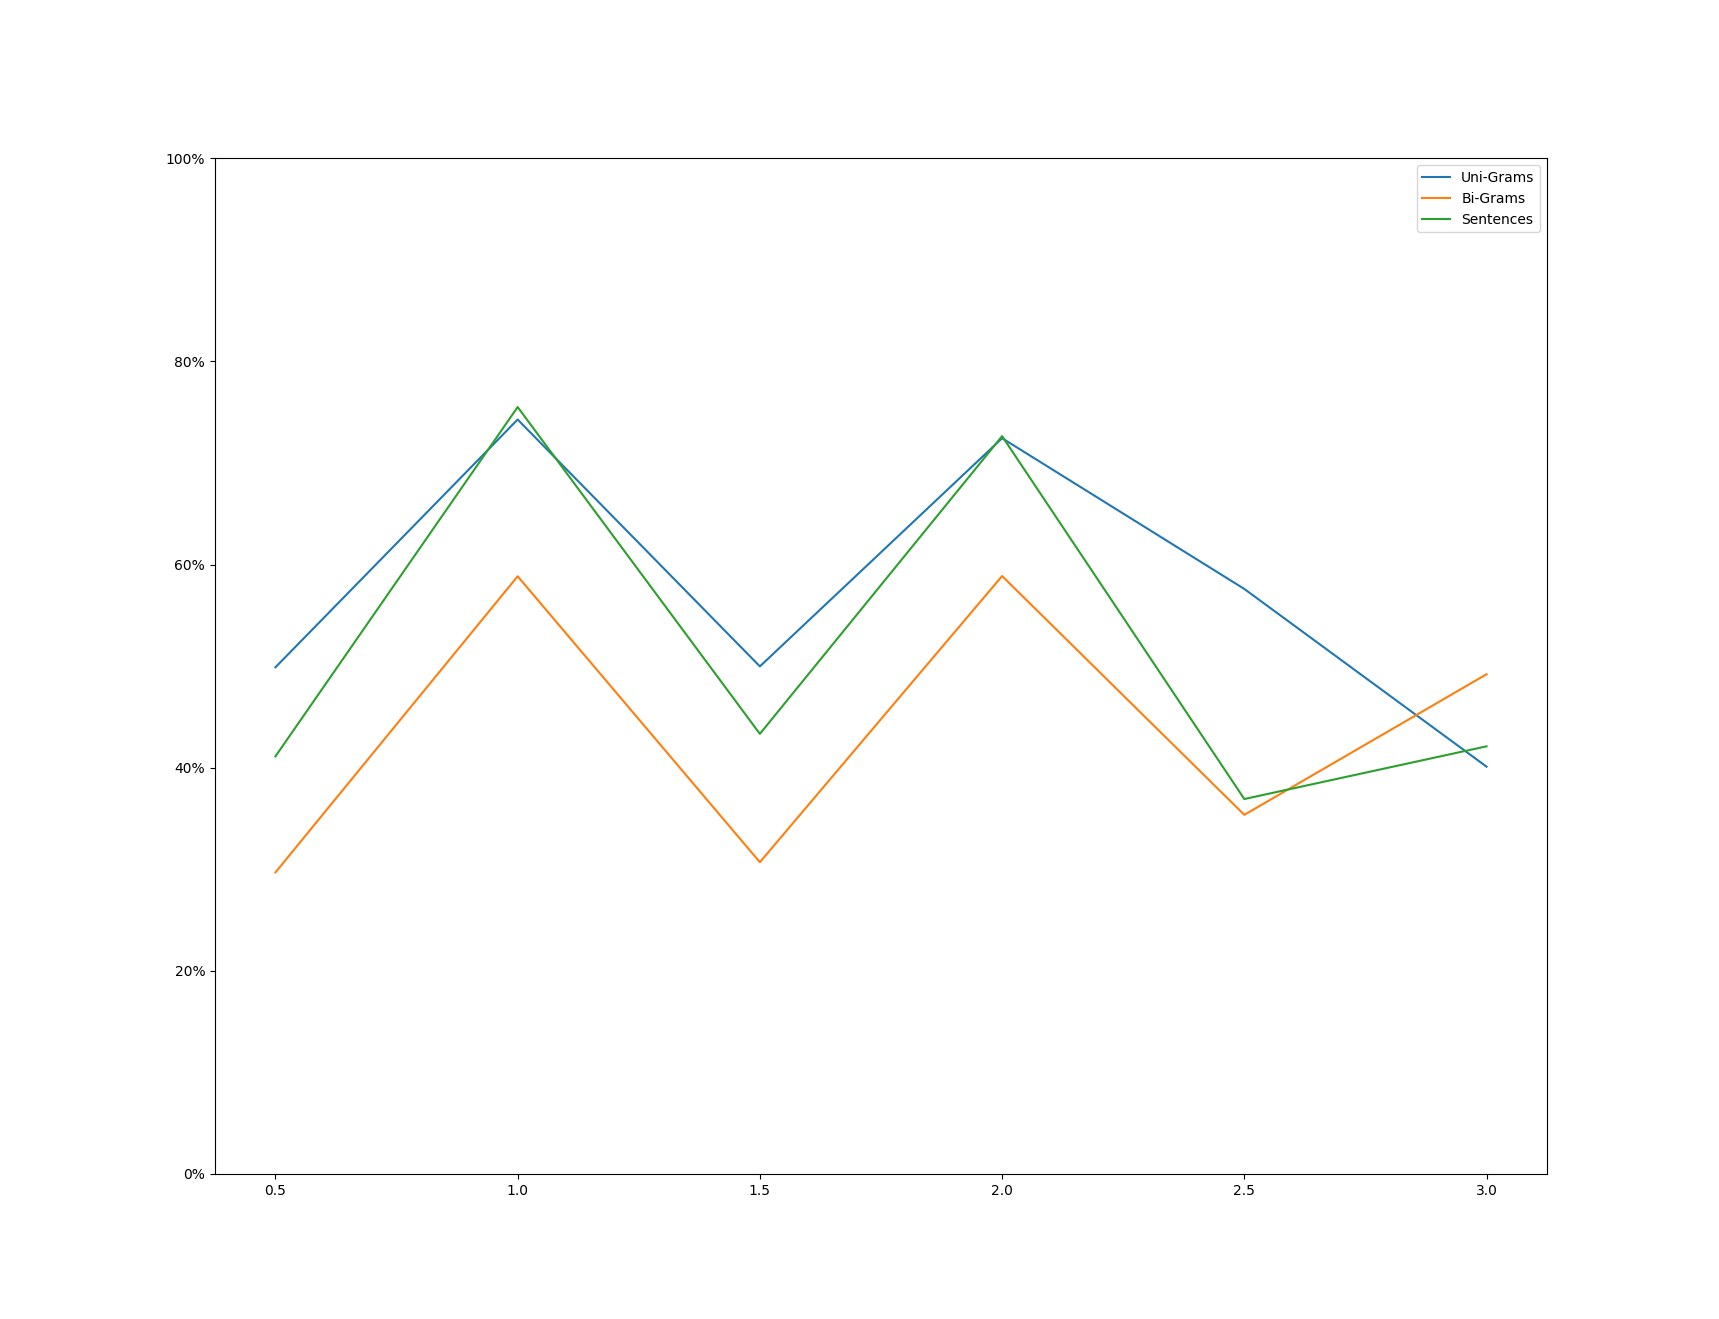
\includegraphics[width=\linewidth]{img/plots/opensubtitles_not_reversed/diversity_perc_plot.png}
	\caption{Development of all uni-, bi-grams and sentences, in percent, that are covered by the top 10 most used instances of each category for the OpenSubtitles model.}
	\label{results:language_model:diversity:opensubtitles}
\end{figure}

\paragraph{Reddit} The plot for the Reddit model (see Figure~\ref{results:language_model:diversity:reddit}) reveals that the language model becomes more diverse over the course of the training until the maximum diversity (minimum in the plot) is achieved when using the 2.0M snapshot. From this point onwards, diversity continously decreases for the rest of the training. This coincides with our opinion, that the model is most optimal when using the 2.0M snapshot. We assume this problematic behavior is caused by the fact, that between the snapshots 1.5M and 2.0M training is within its second epoch. This could lead to an overfitting effect, which worsens the results and diversity of the language used by the model.

\begin{figure}[H]
	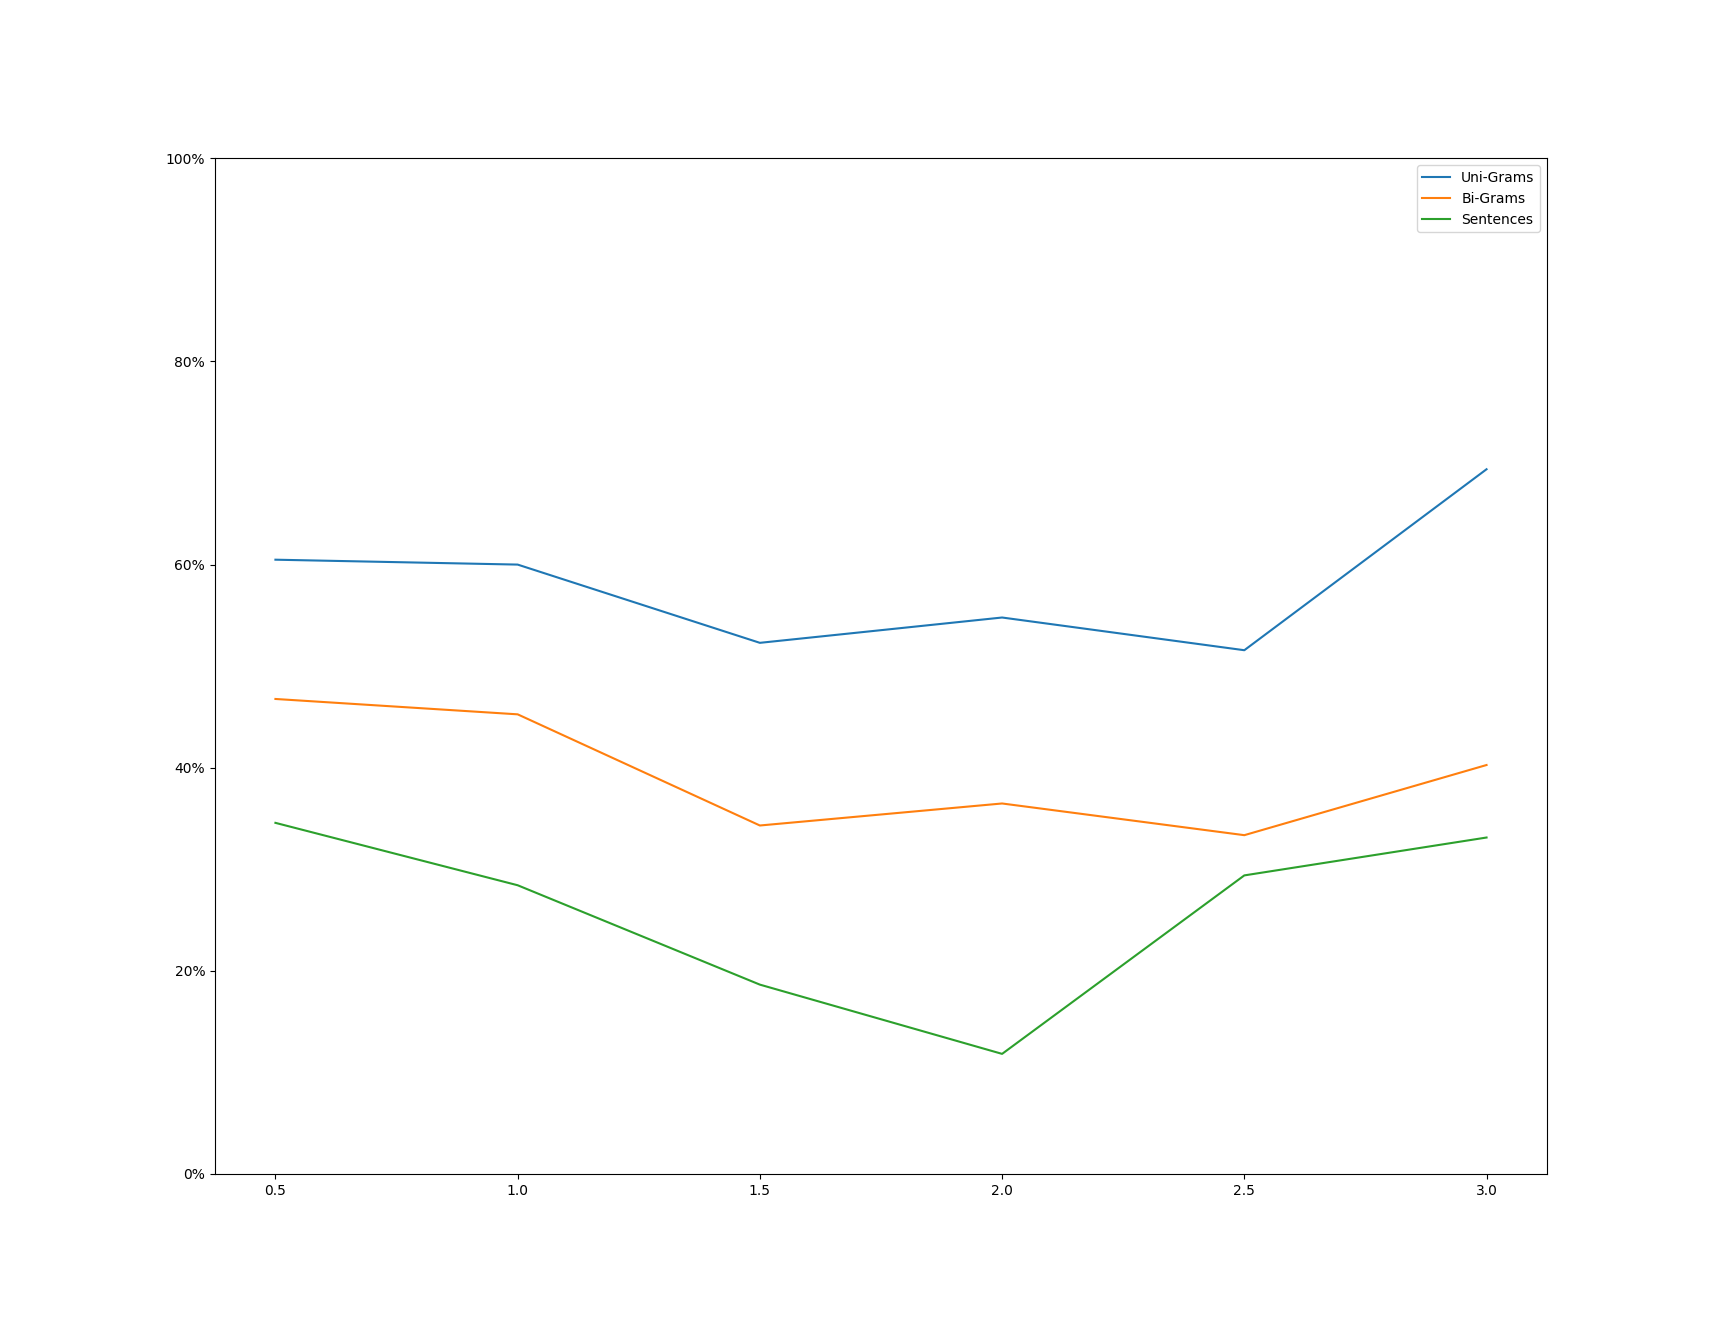
\includegraphics[width=\linewidth]{img/plots/reddit/diversity_perc_plot.png}
	\caption{Development of all uni-, bi-grams and sentences, in percent, that are covered by the top 10 most used instances of each category for the Reddit model.}
	\label{results:language_model:diversity:reddit}
\end{figure}

\subsection{Results}
Our analysis has shown that the distributions of uni- and bi-grams tend to fit the expected distributions better the longer the training advances. However, we found some interesting peculiarities we wanted to analyze with respect to language diversity.

This analysis has shown that the development of the language diversity is in direct relationship to the development of the mentioned n-gram distributions. We were also able to substantiate our subjective feeling, that the OpenSubtitles model improves over time, as the language diversity increase slowly. Additionally, we could also provide evidence that our opinion is correct that the Reddit model has the best performance when using the 1.5M or 2.0M snapshot as these two snapshots have indeed the greatest variety in the used language measured by our statistics. It does not allow us to completely explain the problem with generic responses, but we could show that the share of these generic responses tends to decrease with more training time.

Finally, the analysis showed that iterating over the same dataset multiple times is not recommended, as the Reddit model becomes worse after the snapshot 2.0M. This is particularly apparent when looking at the results of the 3.0M snapshot. Using a regularization technique, such as Dropout~\cite{Nitish:2014} would probably help when using a small dataset which is iterated multiple times.

With this, we conclude the quantitative analysis of the language model and start to do the human evaluation. This evaluation is conducted by comparing our model's results against results from others.

\section{Comparison with Other Models}
We now compare the results of our model with two others. As references we use: The CleverBot\footnote{http://www.cleverbot.com/} chatbot and the results from the paper ``Neural Conversational Model''~\cite{Vinyals:2015}, whose model architecture serves as the base of our model (see Chapter~\ref{methods:architecture}). We test the quality of the responses from our models if confronted with utterances of different types and difficulties. Our expectation is to reveal the strengths and weaknesses of our models.

\subsection{Cleverbot}
\label{results:comparison:cleverbot}
We start with the comparison with the CleverBot. CleverBot is a non-deterministic chatbot, meaning similar inputs can create different outputs if fed at different points in time. The responses listed below were generated at the June 1$^{st}$ between 12am and 15am.

\paragraph{Simple Utterance} We start by using the two simple utterances ``How are you?'' and ``Hi there, i m john!''. As one can see in the Tables~\ref{results:example1_output:OpenSubtitle_compared} and~\ref{results:example1_output:Reddit_compared}, our OpenSubtitles model as well as the CleverBot answered this question with satisfying response. The responses of the Reddit model to the utterance ``Hi there, i m john!'' are rather poor as none of them is really meaningful.
\\
\begin{table}[H]
	\centering
	\begin{adjustbox}{max width=\textwidth}
		\begin{tabular}{ll}
			\toprule
			Input: 	& \texttt{Hi, how are you?}\\
			\midrule
			0.5M: 	& \texttt{how are you ?}\\
			1.0M: 	& \texttt{i m fine}\\
			1.5M:	& \texttt{i m good}\\
			2.0M:	& \texttt{good}\\
			2.5M:	& \texttt{good}\\
			3.0M:	& \texttt{good}\\
			Cleverbot:	& \texttt{I'm good. How are you?}\\
			\bottomrule
		\end{tabular}
	\end{adjustbox}
\caption{Responses from the OpenSubtitles model per snapshot compared to the CleverBot response. The input utterance is ``How are you?''.}
\label{results:example1_output:OpenSubtitle_compared}

\end{table}
\begin{table}[H]
	\centering
	\begin{adjustbox}{max width=\textwidth}
		\begin{tabular}{ll}
			\toprule
			Input: 	& \texttt{Hi there, i m john!}\\
			\midrule
			0.5M:	& \texttt{<unknown>}\\
			1.0M: 	& \texttt{i m not a fan of the <unknown> , but i m not sure if you re a <unknown> .}\\
			1.5M: 	& \texttt{i m not the only one who thought this was a good idea .}\\
			2.0M:	& \texttt{i m a <unknown> !}\\
			2.5M:	& \texttt{i m not your buddy , guy .}\\
			3.0M:	& \texttt{i m not .}\\
			Cleverbot:	& \texttt{So what are you doing?}\\
			\bottomrule
		\end{tabular}
	\end{adjustbox}
	\caption{Responses from the Reddit model per snapshot compared to the CleverBot response. The input utterance is ``Hi there, i m john!''.}
	\label{results:example1_output:Reddit_compared}
\end{table}

\paragraph{Closed Question} In the next step we are comparing responses produced when using a closed question as the utterance. The results are documented in the Tables~\ref{results:example2_output:OpenSubtitle_compared} and~\ref{results:example2_output:Reddit_compared}. With this type of utterance, we intend to evaluate if the models understand a closed question and can respond appropriately.

Our models can respond to closed questions appropriately, as both of them provide useful answers. The CleverBot seems to have problems with this question, probably because it does not understand how the concepts of flying and birds are related.
\\
\begin{table}[H]
	\centering
	\begin{adjustbox}{max width=\textwidth}
		\begin{tabular}{ll}
			\toprule
			Input: 	& \texttt{Can birds fly?}\\
			\midrule
			0.5M: 	& \texttt{no}\\
			1.0M: 	& \texttt{i can t}\\
			1.5M:	& \texttt{yeah , but in the meantime , i can t swim}\\
			2.0M:	& \texttt{no}\\
			2.5M:	& \texttt{i can t}\\
			3.0M:	& \texttt{sure}\\
			Cleverbot:	& \texttt{Some say they can.}\\
			\bottomrule
		\end{tabular}
	\end{adjustbox}
	\caption{Responses to a contextual question from the OpenSubtitles model per snapshot and the CleverBot response.}
	\label{results:example2_output:OpenSubtitle_compared}
\end{table}
\begin{table}[H]
	\centering
	\begin{adjustbox}{max width=\textwidth}
		\begin{tabular}{ll}
			\toprule
			Input: 	& \texttt{Can birds fly?}\\
			\midrule
			0.5M: 	& \texttt{i m not sure if this is a movie , but i m not sure if it s a movie .}\\
			1.0M: 	& \texttt{i can not imagine how much i can get this .}\\
			1.5M:	& \texttt{i m sure he s a <unknown> .}\\
			2.0M:	& \texttt{yes}\\
			2.5M:	& \texttt{yes}\\
			3.0M:	& \texttt{yes}\\
			Cleverbot:	& \texttt{Some of them can.}\\
			\bottomrule
		\end{tabular}
	\end{adjustbox}
	\caption{Responses to a closed question from the Reddit model per snapshot and the CleverBot response.}
	\label{results:example2_output:Reddit_compared}
\end{table}

\paragraph{Knowledge Question}
The next kind of utterance are knowledge questions. With this kind of questions we would like to evaluate if the models have general knowledge. The results can be seen in the Tables~\ref{results:example3_output:OpenSubtitle_compared} and~\ref{results:example3_output:Reddit_compared}.

The responses to the question about the color of the sky show an interesting development. Until the snapshot 2.0M, the responses were not appropriate and did not have any meaningful content\footnote{The response ``the jews'' comes from the fact, that in the beginning of the OpenSubtitles dataset, there are a lot of conversations related to movies about Nazism and world war II.}. However, from the snapshot 2.0M on the model answers in a correct way, even though it replies once with red as the answer, which is obviously wrong. But it also is correct twice, whereas the last response from the 3.0M seems to be the best. The answer of the CleverBot to this question is quite meaningless and is not related at all to the provided question.

The response to the question where the Reddit model lives was answered in a satisfying way, whereby the response of the 2.0M snapshot. It clearly understands the context of the question, as it always answers with a location-related answer. The CleverBot answers this question completely correct.

\begin{table}[H]
	\centering
	\begin{adjustbox}{max width=\textwidth}
		\begin{tabular}{ll}
			\toprule
			Input: 	& \texttt{What color is the sky?}\\
			\midrule
			0.5M: 	& \texttt{the jews}\\
			1.0M: 	& \texttt{it s a}\\
			1.5M:	& \texttt{oh , it s not}\\
			2.0M:	& \texttt{it s the blue}\\
			2.5M:	& \texttt{the red}\\
			3.0M:	& \texttt{blue}\\
			Cleverbot:&\texttt{*Kisses playfully*.}\\
			\bottomrule
		\end{tabular}
	\end{adjustbox}
	\caption{Responses to a knowledge-related question with the OpenSubtitles model per snapshot and the CleverBot response.}
	\label{results:example3_output:OpenSubtitle_compared}
\end{table}
\begin{table}[H]
	\centering
	\begin{adjustbox}{max width=\textwidth}
		\begin{tabular}{ll}
			\toprule
			Input: 	& \texttt{In which country do you live?}\\
			\midrule
			0.5M: 	& \texttt{i m not sure if you re a <unknown> .}\\
			1.0M: 	& \texttt{i live in canada .}\\
			1.5M:	& \texttt{i live in the uk .}\\
			2.0M:	& \texttt{the country}\\
			2.5M:	& \texttt{canada}\\
			3.0M:	& \texttt{sweden}\\
			Cleverbot:&\texttt{The United States.}\\
			\bottomrule
		\end{tabular}
	\end{adjustbox}
	\caption{Responses to a knowledge-related question from the Reddit model per snapshot and the CleverBot response.}
	\label{results:example3_output:Reddit_compared}
\end{table}

\paragraph{Contextual Question} 
With the next question, we want evaluate if the models are capable of using contextual information to build an appropriate response. The results can be seen in the Tables~\ref{results:example4_output:OpenSubtitle_compared} and~\ref{results:example4_output:Reddit_compared}.

As visible below, the OpenSubtitles model has major issues with this kind of utterances, as all the responses are not fitting. The only response with certain usability is the one of the 2.5M model, where at least the correct color is included in the response. The response of the CleverBot is in this case also not of relevance.

The responses of the Reddit model are better fitting to the question, but they are also reasonably poor compared to our expectation. At least the model tries to formulate responses where the two colors of the question are included. The answer of the CleverBot is again useless. This time even less related to the question, compared to the response given by the OpenSubtitles model when using the question.
\\
\begin{table}[H]
	\centering
	\begin{adjustbox}{max width=\textwidth}
		\begin{tabular}{ll}
			\toprule
			Input: 	& \texttt{I wear a blue jeans. What color do my jeans have?}\\
			\midrule
			0.5M: 	& \texttt{<unknown> <unknown>}\\
			1.0M: 	& \texttt{i don t know}\\
			1.5M:	& \texttt{oh , yeah}\\
			2.0M:	& \texttt{i m not a prostitute}\\
			2.5M:	& \texttt{i got a blue blue}\\
			3.0M:	& \texttt{i m not a fan}\\
			Cleverbot:	& \texttt{You don't have any.}\\
			\bottomrule
		\end{tabular}
	\end{adjustbox}
	\caption{Responses to a contextual question from the OpenSubtitles model per snapshot and the CleverBot response.}
	\label{results:example4_output:OpenSubtitle_compared}
\end{table}
\begin{table}[H]
	\centering
	\begin{adjustbox}{max width=\textwidth}
		\begin{tabular}{ll}
			\toprule
			Input: 	& \texttt{I wear a red pullover and blue jeans. What color do my jeans have?}\\
			\midrule
			0.5M: 	& \texttt{i m a big fan of the <unknown> .}\\
			1.0M: 	& \texttt{i m not a fan of the <unknown> , but i do nt know what you re talking about .}\\
			1.5M:	& \texttt{i m a white male and i wear pants .}\\
			2.0M:	& \texttt{i wear a red shirt and i wear glasses .}\\
			2.5M:	& \texttt{i m a red blue and blue blue .}\\
			3.0M:	& \texttt{i m a white male and i have a blue blue shirt .}\\
			Cleverbot:	& \texttt{What is your opinion on President Obama. And don't ask me mine without saying}\\
			& \texttt{yours first!.}\\
			\bottomrule
		\end{tabular}
	\end{adjustbox}
	\caption{Responses to a contextual question from the Reddit model per snapshot and the CleverBot response.}
	\label{results:example4_output:Reddit_compared}
\end{table}

\paragraph{Specific Question}
The next questions are more specific. We are going to ask the OpenSubtitles model a simple mathematical question and the Reddit models a question about the TV series ``Game of Thrones''. The results can be seen in the Tables~\ref{results:example5_output:OpenSubtitle_compared} and~\ref{results:example5_output:Reddit_compared}.

The responses of the OpenSubtitles model are quite clear in the beginning: it does not know the answer or does not understand the question at all. However, the later snapshots (i.e. from 2.0M onwards), it seems to understand that it has to answer with a number. Sadly, the correct results is not included in the generated responses. The CleverBot also does not understand how to answer such a question.

The Reddit model has an interesting twist in its responses. In the beginning, it starts by responding with generic responses which do not seem to have any relation to the TV series. However, the funny response\footnote{``Hodor'' is a character in the ``Game of Thrones'' series who is only capable of saying its own name. In case of danger he starts yelling its name over and over again, which occurs several times throughout the series.} at the end (i.e. ``hodor, hodor, ...'') indicates that it understands the question at least to some degree, even though the response does not contain any actual information about the series. The CleverBot response is a mystery to us, as we could not find any character or other scene in the series where a ``Dani'' is mentioned.
\\
\begin{table}[H]
	\centering
	\begin{adjustbox}{max width=\textwidth}
		\begin{tabular}{ll}
			\toprule
			Input: 	& \texttt{How much is 1 added to 2?}\\
			\midrule
			0.5M: 	& \texttt{i don t know}\\
			1.0M: 	& \texttt{i don t know}\\
			1.5M:	& \texttt{i don t know}\\
			2.0M:	& \texttt{ten dollars}\\
			2.5M:	& \texttt{50}\\
			3.0M:	& \texttt{2}\\
			Cleverbot:	& \texttt{I don't know.}\\
			\bottomrule
		\end{tabular}
	\end{adjustbox}
	\caption{Responses to a mathematical question from the OpenSubtitles model per snapshot and the CleverBot response.}
	\label{results:example5_output:OpenSubtitle_compared}
\end{table}
\begin{table}[H]
	\centering
	\begin{adjustbox}{max width=\textwidth}
		\begin{tabular}{ll}
			\toprule
			Input: 	& \texttt{Can you tell me something about game of thrones?}\\
			\midrule
			0.5M: 	& \texttt{i m not sure if you re a fan of the movie , but i m not sure if you re going to be}\\
			& \texttt{a fan of the}\\
			1.0M: 	& \texttt{i m not sure what you re saying .}\\
			1.5M:	& \texttt{i m not sure if i m going to be watching this .}\\
			2.0M:	& \texttt{i m not sure if you re joking , but i m pretty sure that s the case .}\\
			2.5M:	& \texttt{i m not sure if you re talking about the game or the game , but i think the game}\\
			& \texttt{is a little different .}\\
			3.0M:	& \texttt{hodor hodor hodor hodor hodor hodor hodor hodor hodor hodor hodor hodor hodor hodor }\\
			& \texttt{hodor hodor hodor hodor hodor hodor hodor hodor hodor hodor hodor hodor hodor hodor}\\
			Cleverbot:	& \texttt{Dani is life.}\\
			\bottomrule
		\end{tabular}
	\end{adjustbox}
	\caption{Responses to a question about a TV series from the Reddit model per snapshot and the CleverBot response.}
	\label{results:example5_output:Reddit_compared}
\end{table}

\paragraph{Answers to Statements}
Until now, we have only asked questions to our models. We would now like to see how the responses to statements instead of a questions are. The results can be seen in the Tables~\ref{results:example6_output:OpenSubtitle_compared} and~\ref{results:example6_output:Reddit_compared}.

The responses of the OpenSubtitles model are useful from the snapshot 2.0M onward. Especially the answer for the snapshot 2.0M is interesting, as this seems to indicate that the model has some kind of empathy for the other person in the dialog, expressed in the response ``i m sorry''. The response of the CleverBot signifies that it understands the statement to some degree, but does not know what to answer.

The responses of the Reddit model to the statement that it has a bad opinion are rather poor across all snapshots, with the response from the 1.5M model being the only one which is remotely useful. The response of the CleverBot is a pretty speedy answer in this case.
\\
\begin{table}[H]
	\centering
	\begin{adjustbox}{max width=\textwidth}
		\begin{tabular}{ll}
			\toprule
			Input: 	& \texttt{i invited her to a public reading of my work , but she never came .}\\
			\midrule
			0.5M: 	& \texttt{she was a}\\
			1.0M: 	& \texttt{i don t know}\\
			1.5M:	& \texttt{really ?}\\
			2.0M:	& \texttt{i m sorry}\\
			2.5M:	& \texttt{she s been in a lot of trouble}\\
			3.0M:	& \texttt{she s not a fan}\\
			Cleverbot:	& \texttt{Who?}\\
			\bottomrule
		\end{tabular}
	\end{adjustbox}
	\caption{Responses to a statement from the OpenSubtitles model per snapshot and the CleverBot response.}
	\label{results:example6_output:OpenSubtitle_compared}
\end{table}
\begin{table}[H]
	\centering
	\begin{adjustbox}{max width=\textwidth}
		\begin{tabular}{ll}
			\toprule
			Input: 	& \texttt{Your film taste is bad and your opinion does not interest me!}\\
			\midrule
			0.5M: 	& \texttt{i m not sure what you re saying .}\\
			1.0M: 	& \texttt{i m not your friend , but i m not a fan of the <unknown> .}\\
			1.5M:	& \texttt{i m sorry , i did nt know that .}\\
			2.0M:	& \texttt{i m not a fan of the movie , but i m not sure if you re going to be a fan of the film .}\\
			2.5M:	& \texttt{i m not a fan of the film , but i think it s a good movie .}\\
			3.0M:	& \texttt{i m not sure if you re being sarcastic or not .}\\
			Cleverbot:	& \texttt{And for me your opinion does not matter.}\\
			\bottomrule
		\end{tabular}
	\end{adjustbox}
	\caption{Responses to a statement from the Reddit model per snapshot and the CleverBot response.}
	\label{results:example6_output:Reddit_compared}
\end{table}

\paragraph{Self-Concept} Finally, we have an interesting answer from the Reddit model to the question ``What are you?''. The responses can be seen in Table~\ref{results:example7_output:Reddit_compared}. All snapshots produce bad responses, apart from the last, where it answered that it is a bot. This is an interesting answer because it shows that the model seems to potentially have some kind of self-concept. We cannot explain that, as the model was trained on comments from Reddit discussion about movies and series. Nevertheless, it is an interesting answer to see.

\begin{table}[H]
	\centering
	\begin{adjustbox}{max width=\textwidth}
		\begin{tabular}{ll}
			\toprule
			Input: 	& \texttt{What are you?}\\
			\midrule
			0.5M: 	& \texttt{i m not a fan of the movie , but i m a huge fan of the movie .}\\
			1.0M: 	& \texttt{i m not a fan of the <unknown> , but i m not a fan of the <unknown> .}\\
			1.5M:	& \texttt{i m not .}\\
			2.0M:	& \texttt{i m not .}\\
			2.5M:	& \texttt{i m not .}\\
			3.0M:	& \texttt{i m a bot .}\\
			Cleverbot:	& \texttt{A human, what are you??}\\
			\bottomrule
		\end{tabular}
	\end{adjustbox}
	\caption{Responses to a self-concept question from the Reddit models and the CleverBot response.}
	\label{results:example7_output:Reddit_compared}
\end{table}

Sadly, we were not able to find a similar response when using the OpenSubtitles model.

\subsection{Neural Conversational Model}
\label{results:comparison:ncm}
In this section, we are going to compare the results from the paper ``Neural Conversation Model'' (NCM) with the resulting responses from our models. To compare the responses, we are going to use utterances from the paper and show all the responses from all OpenSubtitles snapshots, but only the (subjectively) best response from the Reddit model, as the NCM model was trained on the OpenSubtitles dataset. The responses can be seen in the Tables~\ref{results:example8_output:Neural_Conversational_Model_compared} to~\ref{results:example14_output:Neural_Conversational_Model_compared}. The categories where the input utterances came from in the paper are noted in the table descriptions. A discussion of the results can be found at the end of this chapter.

In this section, we do not provide individual evaluations to the model responses, as the objective was to gain an overall impression of the quality of responses to individual utterances.

We are only showing a part of the dialogs which were evaluated. All other can be found in Appendix~\ref{apendix:results:compared_with_NCM}.
\\
\begin{table}[H]
	\centering
	\begin{adjustbox}{max width=\textwidth}
		\begin{tabular}{ll}
			\toprule
			Input: 	& \texttt{what year were you born ?}\\
			\midrule
			OpenSubtitle\\
			0.5M: 	& \texttt{a lot of people}\\
			1.0M: 	& \texttt{i was a}\\
			1.5M:	& \texttt{a little}\\
			2.0M:	& \texttt{i was born}\\
			2.5M:	& \texttt{i don t know}\\
			3.0M:	& \texttt{i don t know}\\
			\midrule
			Reddit\\
			2.0M:	& \texttt{i was born in the 90s .}\\
			\midrule
			NCM:	& \texttt{1977 .}\\
			\bottomrule
		\end{tabular}
	\end{adjustbox}
	\caption{Comparison between the NCM model and our OpenSubtitles model when using the utterance ``what year were you born ?'' from the ``Basic''.}
	\label{results:example8_output:Neural_Conversational_Model_compared}
\end{table}

\begin{table}[H]
	\centering
	\begin{adjustbox}{max width=\textwidth}
		\begin{tabular}{ll}
			\toprule
			Input: 	& \texttt{why are we here ?}\\
			\midrule
			OpenSubtitle\\
			0.5M: 	& \texttt{because we were here}\\
			1.0M: 	& \texttt{i don t know}\\
			1.5M:	& \texttt{i don t know}\\
			2.0M:	& \texttt{i m sorry}\\
			2.5M:	& \texttt{we re here}\\
			3.0M:	& \texttt{we re here}\\
			\midrule
			Reddit\\
			1.5M:	& \texttt{because we are nt .}\\
			\midrule
			NCM:	& \texttt{i ’m not sure .}\\
			\bottomrule
		\end{tabular}
	\end{adjustbox}
	\caption{Comparison between the NCM model and our OpenSubtitles model when using the utterance ``why are we here ?'' from the ``Basic'' category.}
	\label{results:example9_output:Neural_Conversational_Model_compared}
\end{table}
\begin{table}[H]
	\centering
	\begin{adjustbox}{max width=\textwidth}
		\begin{tabular}{ll}
			\toprule
			Input: 	& \texttt{are you a leader or a follower ?}\\
			\midrule
			OpenSubtitle\\
			0.5M: 	& \texttt{no}\\
			1.0M: 	& \texttt{i m not a}\\
			1.5M:	& \texttt{i m sorry}\\
			2.0M:	& \texttt{i m not a prostitute}\\
			2.5M:	& \texttt{i m a}\\
			3.0M:	& \texttt{i m a}\\
			\midrule
			Reddit\\
			2.0M:	& \texttt{i m a cyborg .}\\
			\midrule
			NCM:	& \texttt{i'm a leader .}\\
			\bottomrule
		\end{tabular}
	\end{adjustbox}
	\caption{Comparison between the NCM model and our OpenSubtitles model when using the utterance ``are you a leader or a follower ?'' from the ``General Knowledge Q\&A'' category.}
	\label{results:example10_output:Neural_Conversational_Model_compared}
\end{table}
\begin{table}[H]
	\centering
	\begin{adjustbox}{max width=\textwidth}
		\begin{tabular}{ll}
			\toprule
			Input: 	& \texttt{how much is ten minus two ?}\\
			\midrule
			OpenSubtitle\\
			0.5M: 	& \texttt{four}\\
			1.0M: 	& \texttt{ten}\\
			1.5M:	& \texttt{two , two , three}\\
			2.0M:	& \texttt{ten dollars}\\
			2.5M:	& \texttt{ten}\\
			3.0M:	& \texttt{ten}\\
			\midrule
			Reddit\\
			2.0M:	& \texttt{i m not sure how much i m going to get downvoted to hell .}\\
			\midrule
			NCM:	& \texttt{seventy - two .}\\
			\bottomrule
		\end{tabular}
	\end{adjustbox}
	\caption{Comparison between the NCM model and our OpenSubtitles model when using the utterance ``how much is ten minus two ?'' from the ``General Knowledge Q\&A'' category.}
	\label{results:example11_output:Neural_Conversational_Model_compared}
\end{table}
\begin{table}[H]
	\centering
	\begin{adjustbox}{max width=\textwidth}
		\begin{tabular}{ll}
			\toprule
			Input: 	& \texttt{what is the color of a yellow car ?}\\
			\midrule
			OpenSubtitle\\
			0.5M: 	& \texttt{a <unknown> ?}\\
			1.0M: 	& \texttt{it s a}\\
			1.5M:	& \texttt{what ?}\\
			2.0M:	& \texttt{it s a blue blue}\\
			2.5M:	& \texttt{it s a blue}\\
			3.0M:	& \texttt{it s a yellow}\\
			\midrule
			Reddit\\
			2.5M:	& \texttt{the yellow yellow yellow yellow yellow yellow yellow yellow}\\
					& \texttt{yellow yellow yellow yellow yellow yellow yellow yellow yellow}\\
					& \texttt{yellow yellow yellow yellow yellow yellow yellow yellow yellow yellow}\\
					\midrule
			NCM:	& \texttt{yellow .}\\
			\bottomrule
		\end{tabular}
	\end{adjustbox}
	\caption{Comparison between the NCM model and our OpenSubtitles model when using the utterance ``what is the color of a yellow car ?'' from the ``General Knowledge Q\&A'' category.}
	\label{results:example12_output:Neural_Conversational_Model_compared}
\end{table}
\begin{table}[H]
	\centering
	\begin{adjustbox}{max width=\textwidth}
		\begin{tabular}{ll}
			\toprule
			Input: 	& \texttt{what is the purpose of existence ?}\\
			\midrule
			OpenSubtitle\\
			0.5M: 	& \texttt{the jews}\\
			1.0M: 	& \texttt{i don t know}\\
			1.5M:	& \texttt{you re just a fucking boy , man}\\
			2.0M:	& \texttt{i don t know}\\
			2.5M:	& \texttt{i m sorry}\\
			3.0M:	& \texttt{i m not sure}\\
			\midrule
			Reddit\\
			1.5M:	& \texttt{i m not sure if you re joking or not , but i m sure you re }\\
			& \texttt{not familiar with the word .}\\
			\midrule
			NCM:	& \texttt{to find out what happens when we get to the planet earth .}\\
			\bottomrule
		\end{tabular}
	\end{adjustbox}
	\caption{Comparison between the NCM model and our OpenSubtitles model when using the utterance ``what is the purpose of existence ?'' from the ``Philosophical Q\&A'' category.}
	\label{results:example13_output:Neural_Conversational_Model_compared}
\end{table}

\begin{table}[H]
	\centering
	\begin{adjustbox}{max width=\textwidth}
		\begin{tabular}{ll}
			\toprule
			Input: 	& \texttt{what is the purpose of being intelligent?}\\
			\midrule
			OpenSubtitle\\
			0.5M: 	& \texttt{the jews}\\
			1.0M: 	& \texttt{i don t know}\\
			1.5M:	& \texttt{i don t know}\\
			2.0M:	& \texttt{i don t know}\\
			2.5M:	& \texttt{i don t know}\\
			3.0M:	& \texttt{i don t know}\\
			\midrule
			NCM:	& \texttt{to find out what it is .}\\
			\bottomrule
		\end{tabular}
	\end{adjustbox}
	\caption{Comparison between the NCM model and our OpenSubtitles model when using the utterance ``what is the purpose of being intelligent?'' from the ``Philosophical Q\&A'' category.}
	\label{results:example20_output:OpenSubtitle}
\end{table}


\begin{table}[H]
	\centering
	\begin{adjustbox}{max width=\textwidth}
		\begin{tabular}{ll}
			\toprule
			Input: 	& \texttt{what are the things that i do to be immoral?}\\
			\midrule
			OpenSubtitle\\
			0.5M: 	& \texttt{i don t know}\\
			1.0M: 	& \texttt{i don t know}\\
			1.5M:	& \texttt{what s the big idea ?}\\
			2.0M:	& \texttt{i don t know}\\
			2.5M:	& \texttt{i m a}\\
			3.0M:	& \texttt{i m not a criminal}\\
			\midrule
			Reddit\\
			2.5M:	& \texttt{i think you re missing the point .}\\
			& \texttt{i don ’t know .}\\
			\midrule
			NCM:	& \texttt{to find out what happens when we get to the planet earth .}\\
			\bottomrule
		\end{tabular}
	\end{adjustbox}
	\caption{Comparison between the NCM model and our OpenSubtitles model when using the utterance ``what are the things that i do to be immoral?'' from the ``Morality'' category.}
	\label{results:example14_output:Neural_Conversational_Model_compared}
\end{table}

\subsection{Results}
In conclusion, our model is not as poos as expected by looking at the problems with the metrics and the generic responses caused by an undiversified language model.

In comparison to the CleverBot, our model provided several responses which were clearly superior in quality. But there were also cases where the CleverBot outperformed our model. This is probably probably related to the fact that the CleverBot works by fuzzily searching already witnessed conversations. This means, that if a conversation about a certain topic does not exist, the CleverBot has no facilities to create a meaningful answer. In contrast, our model instead has the ability to ``understand'' what is said and, hence can at least try to answer. Such an example would be the mathematical question ``How much is 1 added to 2?'', where the CleverBot simply answered ``I don't know'' and our model started to respond with numbers, even though the result was incorrect.

When comparing our models to the NCM model, one main issue of the model quickly becomes visible: The size of the model. For easily understandable utterances, the responses of our models are almost or as good as the responses from the NCM model. But if the utterances become more complicated, especially when it comes to philosophical or morality questions, our model starts to respond worse than the NCM model. This is, as said, not a real surprise, because our model is only half the size of the NCM model. Nevertheless, we conclude that our model is not superior, but in some regards of comparable quality as the NCM model.

\section{Beam-Search}
\label{results:beam_search}
There are always some poor responses shown in the previous chapter. We would like to use our beam-search implementation as described in Chapter~\ref{fundamentals:decoding_approaches} to evaluate if this can help to increase response quality. We will evaluate this for three different examples, and evaluate if the responses generated by the beam-search decoder are superior to the responses of the greedy decoder. The evaluation was performed subjectively as usually the best answer does not necessarily correlate with the resulting log-probability score. This analysis is exemplarily done with the OpenSubtitles 3.0M model and a beam-width of $200$.

We only list the subjectively best responses here. All other responses can be found in Appendix~\ref{apendix:results:Beam-search-200:OpenSubtitle}. This has to do with the fact, that the subjectively best answer is usually not the best answer found when looking at the log-probability scores.

\paragraph{``what year were you born?''} The responses of the greedy decoder to this question can be found in the Table~\ref{results:example8_output:Neural_Conversational_Model_compared}. The original answers of the OpenSubtitles model were all reasonably poor, and it seemed that the model did not fully understand the question.

However, when using the beam-search decoder, there are several useful responses, such as ``1991'', ``last year'' or ``five years ago''. These responses are much better than the results initially generated by the greedy decoder. However, none of them is the highest ranked response and, hence is not returned by the model as the answer of choice. We provide a possible explanation for this anomaly later.

\paragraph{``i wear a blue jeans. what color do my jeans have?''} The second question was also answered pretty poorly initially. The results of the greedy decoder can be found in Table~\ref{results:example4_output:OpenSubtitle_compared}. The best response was delivered by the 2.5M model and was ``i got a blue blue'', which, at least, contains the searched color.

When using beam-search, better responses can be found. Such responses include ``blue'' and ``you know that''.

\paragraph{``what is the purpose of being intelligent?''} Finally, we wanted to explore a more complicated question from the moral section of the NCM paper with beam-search. The responses of the greedy decoder can be found in Table~\ref{results:example4_output:OpenSubtitle_compared}. All responses are of inferior quality and only consist of generic responses, such as ``i don t know''.

When using beam-search, several interesting responses were produced, fitting for such a philosophical question, such as ``well, it s complicated'', ``you can t know'' and ``well , it s nothing.''

\paragraph{Beam-Search Helps} The responses become much more diverse when using the beam-search decoder. The key problem is to choose the best response from the 200 generated responses. Per algorithm, the sum of the logarithmic probabilities at each step in the beam is used. However, this mechanism does not provide the answers we subjectively selected as ``best'' from the list. We are not quite sure if this is a problem related to the fact that the decoder was trained in a greedy fashion, but response generation was augmented with beam search, which might not be fully compatible. The implementation of beam-search was validated and is correct, as when beam-size is set to 1, answers are the same as when using the greedy decoder. Nevertheless, the implementation provided us insight into the inner mechanics of the model and we were able to find better responses than with the greedy decoder, even though such had to be selected from the list of responses manually

\section{Thought Vectors for Input Sequences} After the encoder has processed the entire input sequences, it forwards the thought vector to the decoder to construct the output sequence (see Chapter~\ref{fundamentals:seq2seq}). As this is the only direct connection of the encoder to the decoder, the encoder must ``encode'' all information into this thought vector. Hence, the thought vector hence represents an embedding of an input sequence in an $n$ dimensional vector space, where $n$ stands for the size of the thought vector. If we project the vectors into two dimensions via PCA, sentences with similar meanings should be clustered. That would substantiate that the models have a semantic understanding of the contents of these sentences.

To analyze the embeddings, we collect them for 15 different sample sentences and create respective thought vectors. We do this with both models and project the vectors via PCA into two-dimensional space. The results of this projection can be see in Figure~\ref{results:thougth_vectors:embeddings:opensubtitles} and~\ref{results:thougth_vectors:embeddings:reddit} below.

\begin{figure}[!tb]
	\centering
	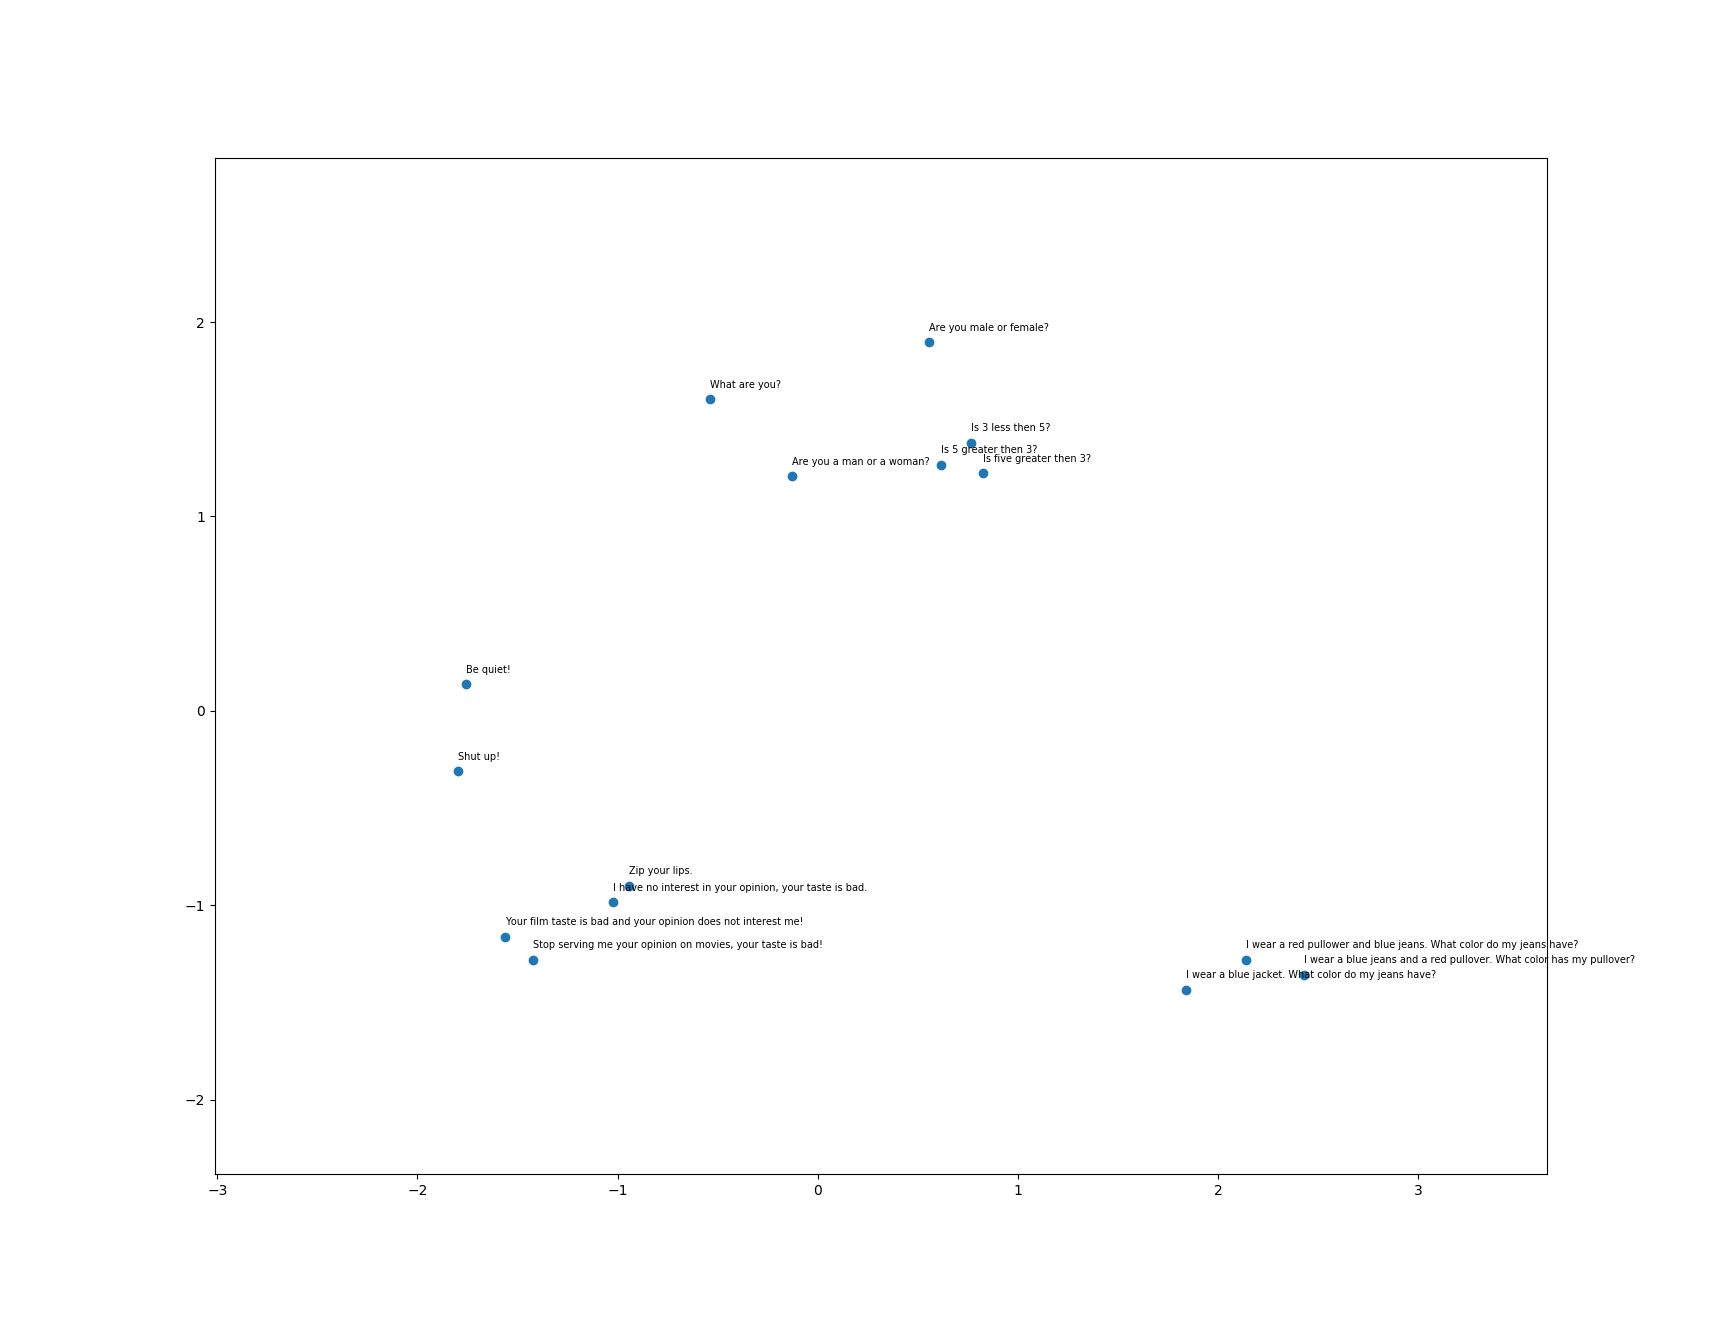
\includegraphics[width=14cm]{img/opensubtitles_thought_vector_embeddings.png}
	\caption{The projected thought vectors for 15 different sentences when using the OpenSubtitles 3.0M model. PCA was used for the projection.}
	\label{results:thougth_vectors:embeddings:opensubtitles}
\end{figure}

\begin{figure}[H]
	\centering
	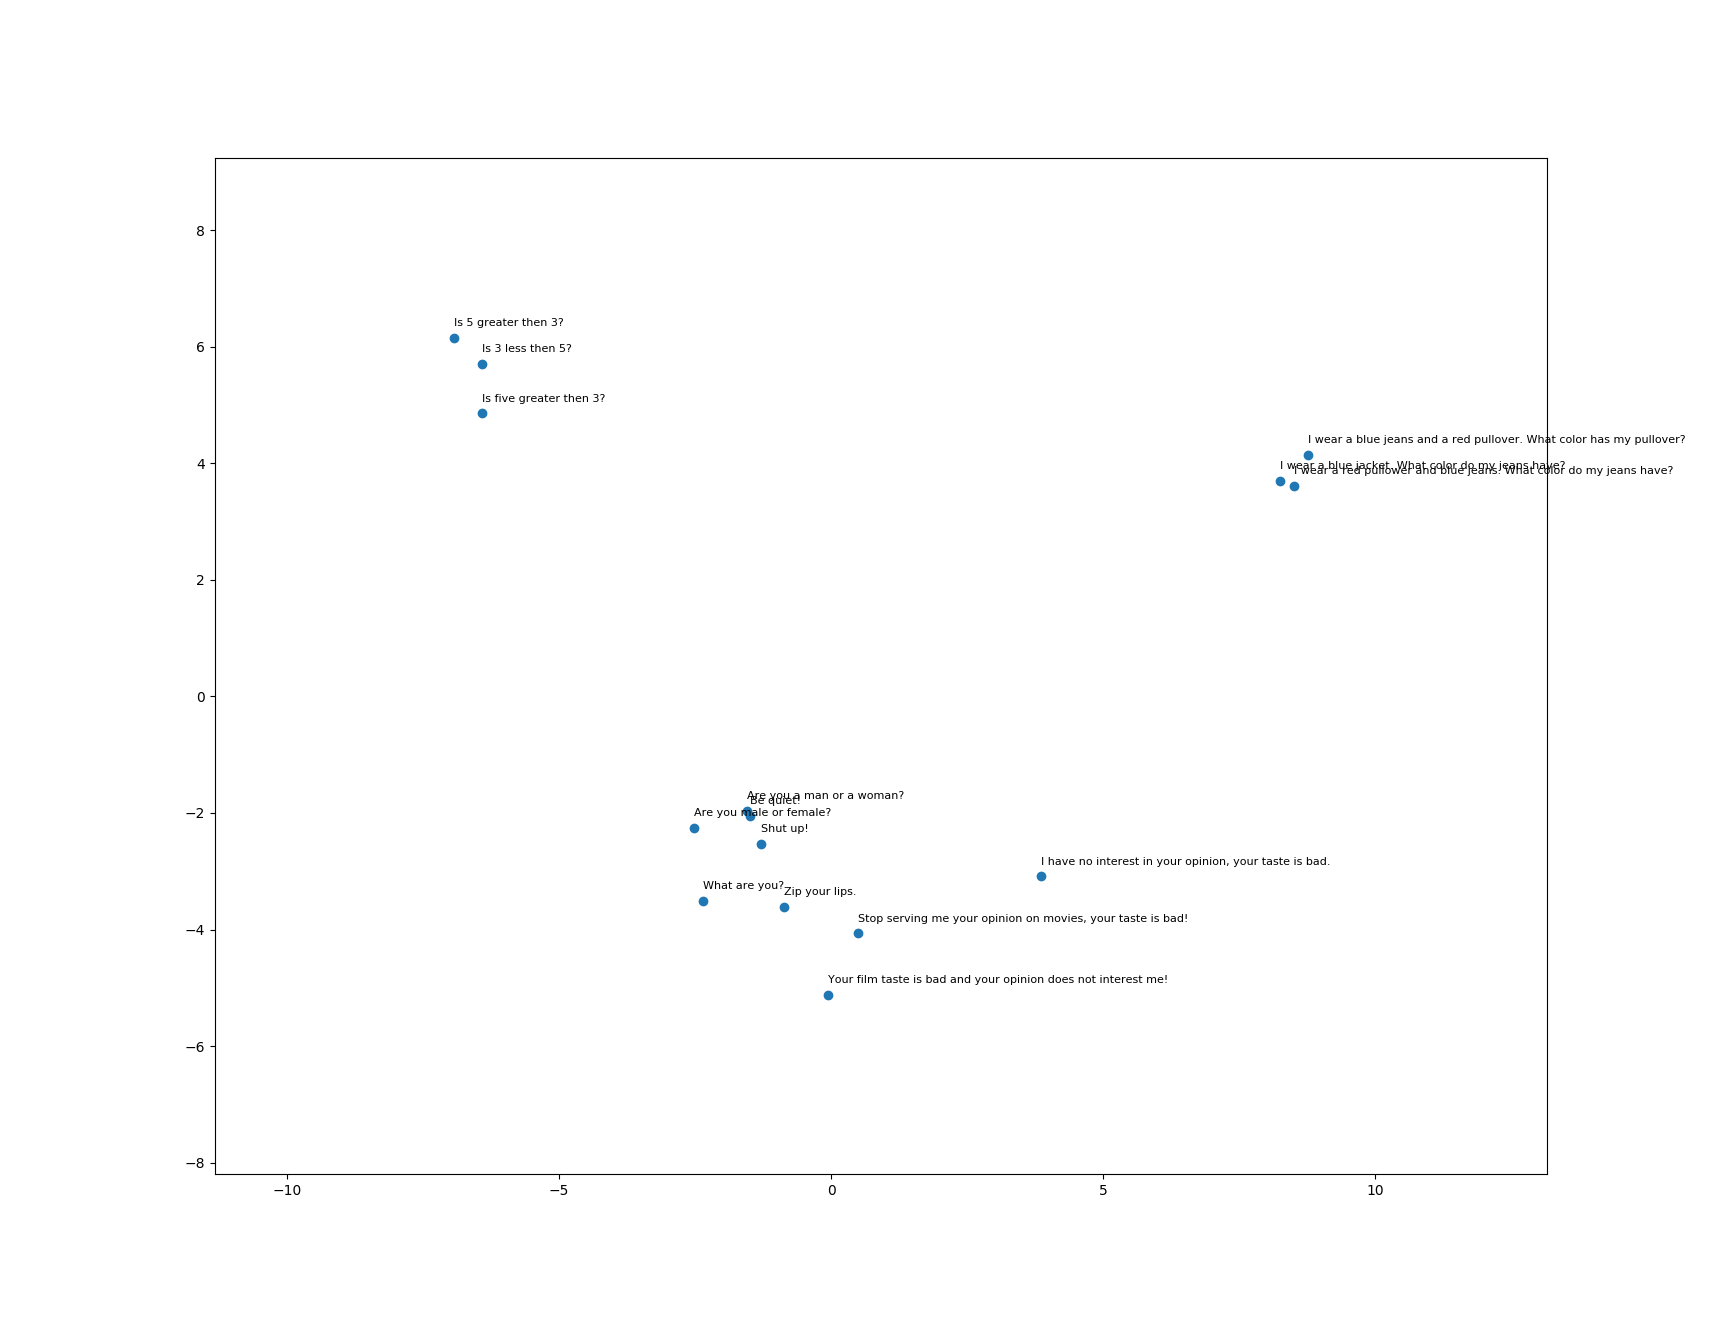
\includegraphics[width=14cm]{img/reddit_thought_vector_embeddings.png}
	\caption{The projected thought vectors for 15 different sentences when using the Reddit 2.0M model. PCA was used for the projection.}
	\label{results:thougth_vectors:embeddings:reddit}
\end{figure}

Both of the models seem to have no problems understanding direct sentences where the content is unambiguous (e.g. ``I have no interest in your opinion on movies, your taste is bad!''). This can be seen because similar sentences are clustered closely in the projected space. However, when it comes to curses and questions regarding the gender, the OpenSubtitles model starts to struggle, which can be seen by taking a look at the respective points in the projected space. The questions regarding the gender or the curses are scattered throughout the space, even though they should have been embedded closely to each other. The Reddit model seems to have less problems with this, as the embeddings for these sentences are clustered tighter. Interestingly, the Reddit model embeds the sentences with curses close to the sentences regarding the gender.

In general, it appears as the models have an understanding of these different sentences as most of the points are clustered, if they contain similar content. From this, we conclude that our models have, at least to a certain degree, an understanding of the meaning of utterances.

\section{Soft-Attention}
\label{results:soft_attention}
In the last part, we take a look at the soft-attention mechanism (see Chapter~\ref{fundamentals:soft_attention}) and analyze if the model benefits from its use by looking at the resulting attention weights. We do not expect significant advantages, as Vinyals and Le already notice in their paper~\cite{Vinyals:2015}. The visualizations are generated by feeding an utterance to our models and then visualizing the resulting attention weights (see Chapter~\ref{fundamentals:soft_attention}) in a heat-map over the different time steps of the decoding process. As utterances we use three different examples, one general question, one mathematical question and a an example which consists of two sentences with a relative pronoun in the second sentence, which refers to the subject of the first sentence.

We perform this analysis on the OpenSubtitles 3.0M and the Reddit 2.0M snapshots.

\paragraph{Attention Visualizations} The visualizations of the attention weights can be seen in Figures~\ref{results:attention:example3:opensubtitles-3M} and~\ref{results:attention:example3:reddit}. Additional visualizations of the same kind are located in Appendix~\ref{appendix:soft_attention}.

Clearly visible, the generated attention weights do not show a significant alignment with important words from the input utterance. For example when looking at the input utterance ``anna is 18 years old. how old is she?'' (Figure~\ref{results:attention:example3:reddit}), we would expect that the decoder would place a large attention weight on the thought vector when the actual age of the person is processed. However, this is not the case for any of the output words.

\begin{figure}[H]
	\centering
	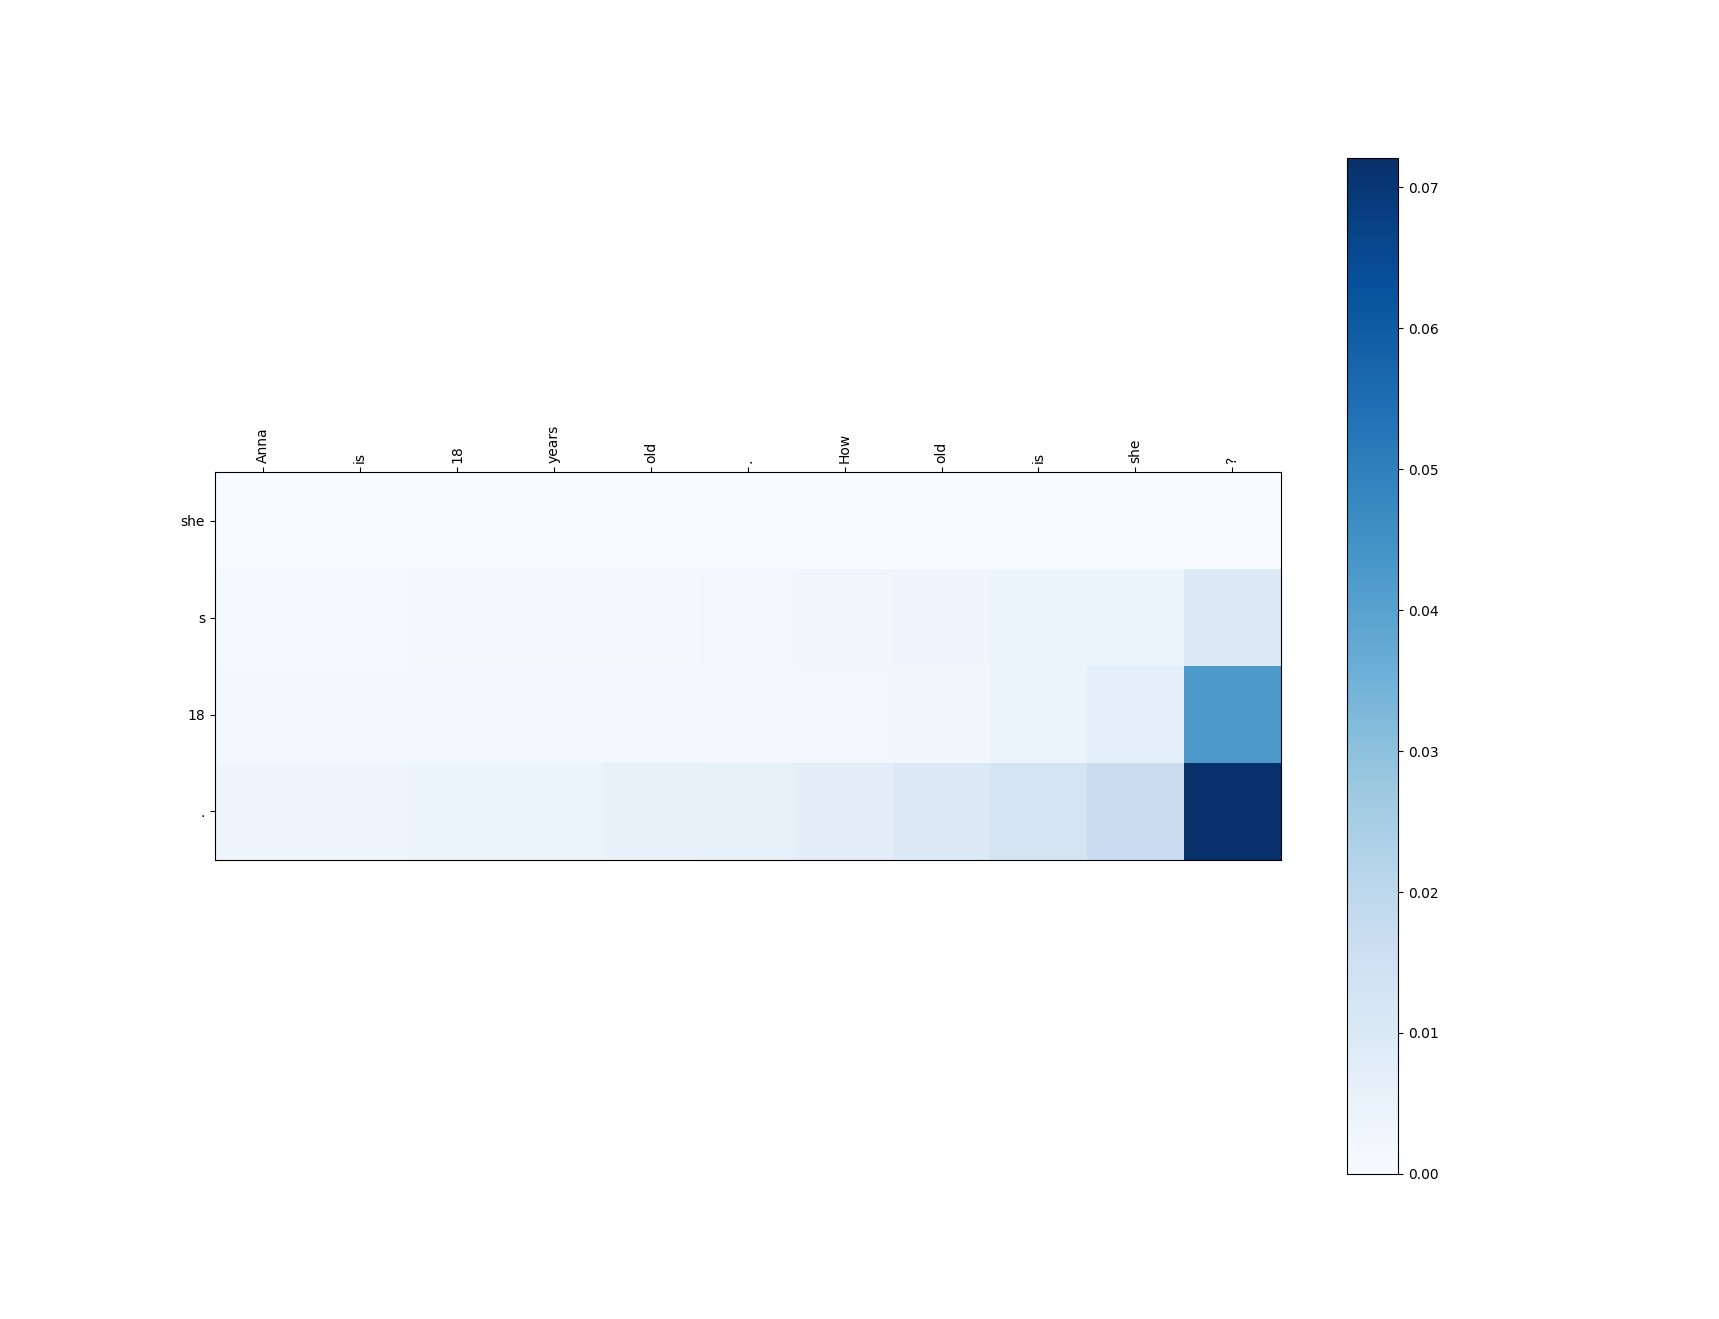
\includegraphics[width=10cm]{img/attention/attention_visualization3_reddit_2m.png}
	\caption{Visualization of the attention weights when using the utterance ``anna is 18 years old. how old is she?". On the x-axis, the input utterance is placed at the top of the chart from left to right. On the y-axis, the response from the model is placed from top to bottom. Each square in the heatmap corresponds to the attention weight the decoder computed for the thought vector of the corresponding word (x-axis) when producing the corresponding response word (y-axis). The Reddit 2.0M was used here.}
	\label{results:attention:example3:reddit}
\end{figure}

A second example, where attention does not compute meaningful alignments, is shown in Figure~\ref{results:attention:example3:opensubtitles-3M}. Here it is the same problem as before, the attention weights do not align with the important thought vectors from the input utterance.

\begin{figure}[H]
	\centering
	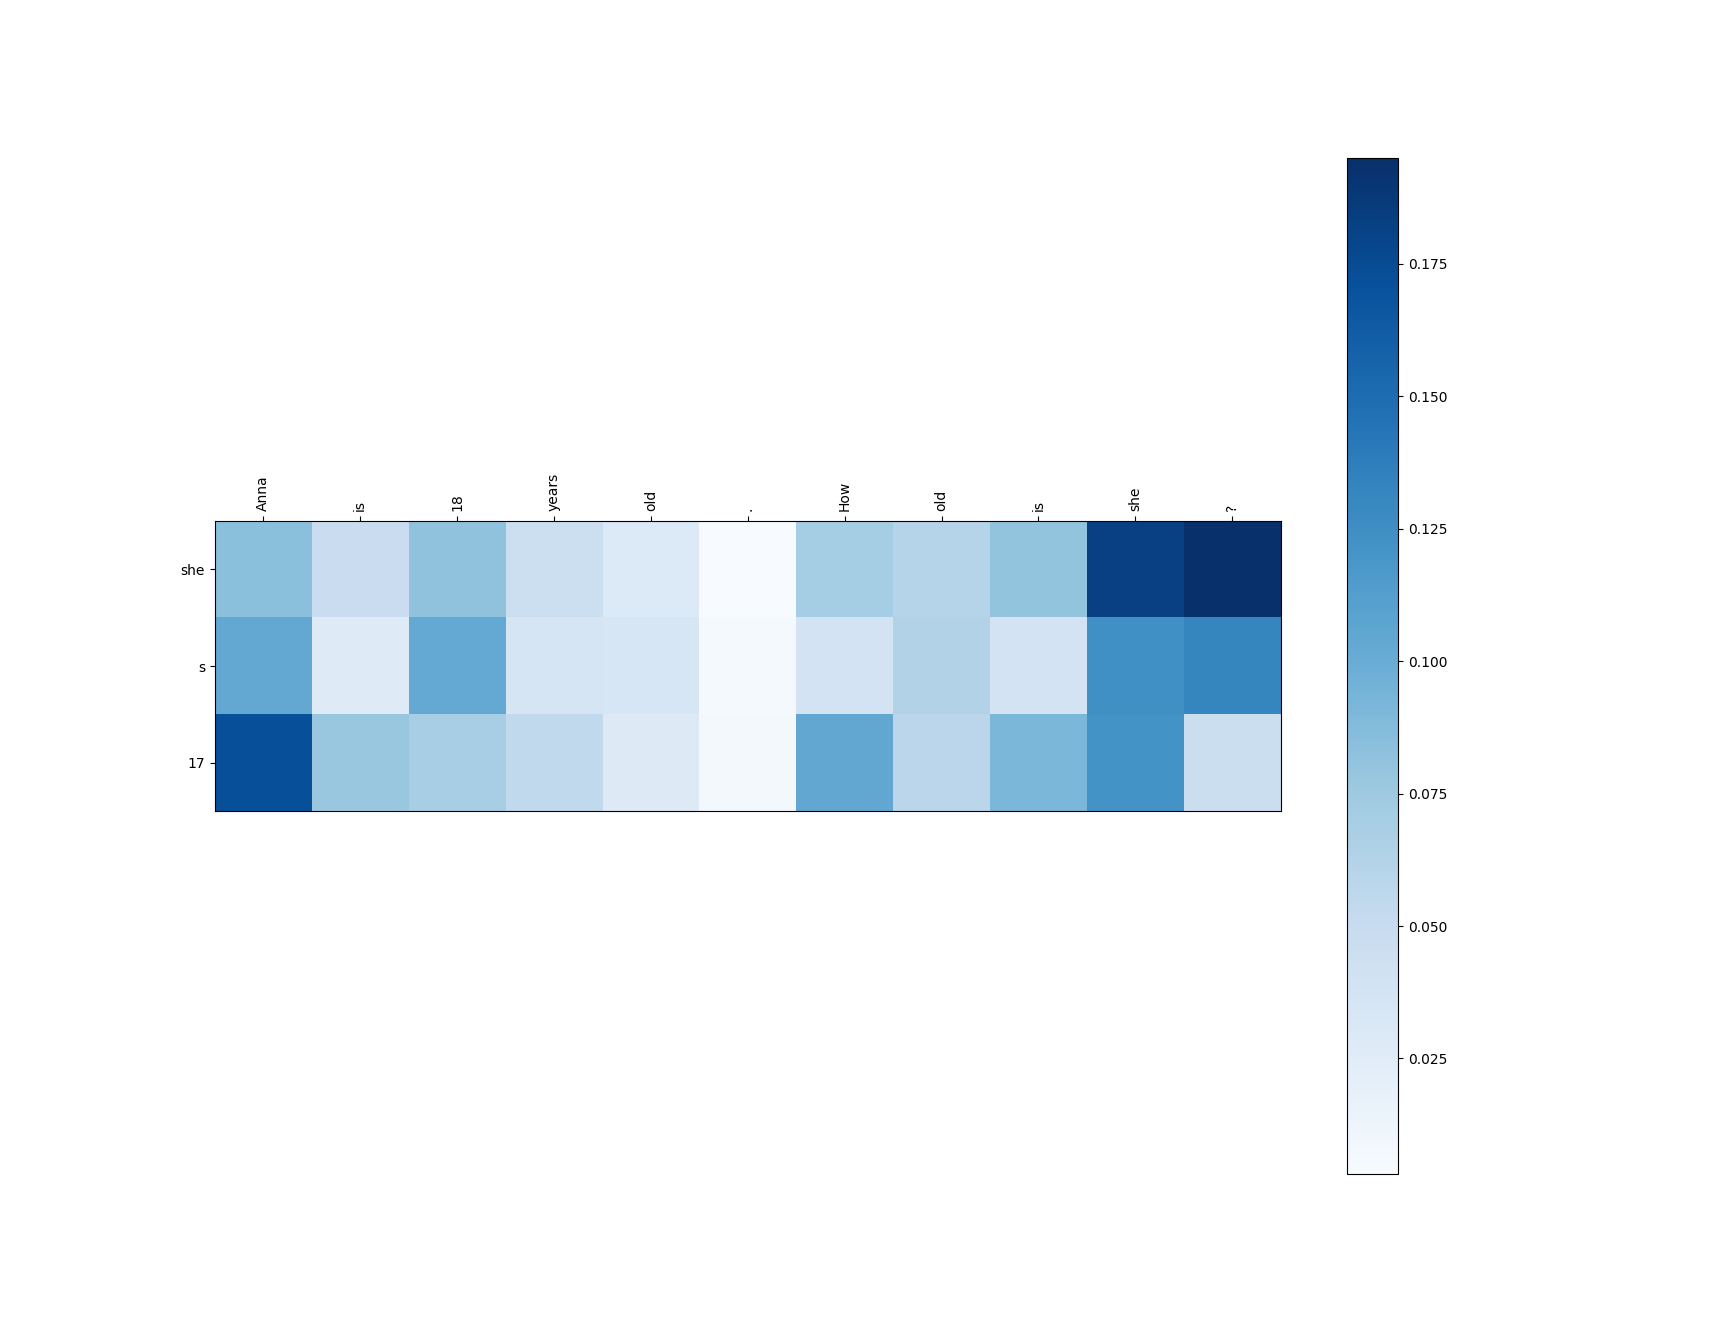
\includegraphics[width=10cm]{img/attention/attention_visualization3_OpenSubtitle-3M.png}
	\caption{Visualization of the attention weights when using the utterance ``anna is 18 years old. how old is she?". On the x-axis, the input utterance is placed at the top of the chart from left to right. On the y-axis, the response from the model is placed from top to bottom. Each square in the heatmap corresponds to the attention weight the decoder computed for the thought vector of the corresponding word (x-axis) when producing the corresponding response word (y-axis). The OpenSubtitles 3.0M was used here.}
	\label{results:attention:example3:opensubtitles-3M}
\end{figure}

From this quick analysis, we can reaffirm that the soft-attention mechanism does not seem to help to improve the decoders comprehension in conversational models, as Vinyals and Le also noticed.


\chapter{Conclusion}

We started this thesis with the goal to build an end-to-end dialog system using the architecture and technologies from the ``Neural Conversational Model'' paper of Vinyals and Le~\cite{Vinyals:2015}. Our main idea was to build such a system, but on a much smaller scale. The goal of this reduction was to fit the resulting system onto a single GPU, instead of using the ressources of a whole server as they did in the paper.

The implementation of our system was a big challenge, but it allowed us to learn more about the details on how such systems are implemented on a much lower level and taught us many different things, including how a computational graph works, the inner workings of sequence-to-sequence models and we even had the chance to implement an in-graph beam-search decoder at the end.

Due to difficulties with several different APIs from the TensorFlow framework, it took a much longer time than expected until we had our first, running version of the system. But, after all the trouble, after more than half of the semester has already passed, we could finally start the training of our models on the two datasets, namely the Reddit comment and the OpenSubtitles dataset. We have decided to use this two datasets for two reasons: First, our initial goals was build a system with which we could talk about movie related topics. The second reason was, that these two datasets represent two different types of language, spoken and written. Handling and preprocessing both of these datasets was pretty big challenge, because both of them are huge, bigger than anything we have handled before. The Reddit dataset also imposed another difficulty because we had to reconstruct the original discussions by using tree structure.

After we have obtained both datasets and a working version of the system we started to evaluate how big in terms of size we could make our models so that they would still fit onto a single GPU. This took some time, as a lot of different hyperparameters are responsible for the final memory consumption.

When we found the maximum achievable size for the models, we started their training. To keep track of the development of the models throughout the training, we took snapshots of them at six distinct points in time. After more than three weeks of training time, we had our six snapshots and could start by analyzing the results.

At first glance, everything looked fine and the loss and perplexity values on the training datasets suggested that the training went fine overall. There were differences in the speed and way how the models learned throughout the time span of the training, especially apparent was the high variance in the metrics for OpenSubtitles which we had not seen with the Reddit model. We concluded that this had to do with the differently structured datasets, as the Reddit dataset has a clear structure implied by the structure of the conversations on Reddit. This was different with the OpenSubtitles dataset, as we had no information about turn-taking or structure of the conversations.

We then went on and started evaluating our models with the respective test datasets with the mentioned loss and perplexity metrics. Additionally, we also tried a new metric based on the recently published Sent2Vec library. At first, we were shocked by the results and thought that the whole experiment has failed. However, we could then find several reasons for why the models did not show the performance we first expected. Our first finding was, that the cross-entropy loss function and the related perplexity metrics might not be the most suitable metrics for measuring the performane of a conversational dialog system, as the range of possible responses which are appropriate is extremely huge. We were aware of this problem from the beginning, why we put some thoughts into a new metric based on the Sent2Vec library. However, the results of assessing the performance of the models with this metric did also not bring the good results we wished to achieve. One interesting fact we could extract from the results was, that the Reddit model was twice as good as the OpenSubtitles model in this evaluation. We concluded that this has to do with the differences between spoken and written language, which are both present in our datasets. Overall, the results did in our opinion not reflect the performance of the models because we had already talked to them and thought that the results were not that bad. We then started to investigate into the language models to find the reason for the poor results.

Our first try to find a reason for the poor results was to look at the generated responses. We quickly noticed the lack variety in the responses. Instead our models often generated generic sentences, such as ``i don t know'' and ``i m not sure''. We started to investigate into the how our models adopted the language models from the training datasets. We did this by looking at the development of uni- and bi-gram distributions over the time span of the training. This revealed, that the learning process of the OpenSubtitles model differed from the learning process of the Reddit model. It exhibited much more variance, which we concluded is due to the much more noisey dataset in comparison to the Reddit dataset. It also revealed, that it is not recommendable to use smaller dataset and iterate over it multiple times, as we did with the Reddit model. The result was, that the snapshots of the later Reddit models showed a much poorer performance overall, for metrics and if we talked to the model directly.

We still had the assumption that the generic responses could be explained somehow. This is why we did another analysis were we analyzed the usage frequencies of the top 10 most used uni-, bi-grams and sentences in the outputs when using the test datasets. Our intention with this analysis was that we wanted to see how the language variety evolves over time. The results showed that the amount of generic responses decrease over time. We could also confirm our subjection impression that the models have a tendency to become better over time, especially the OpenSubtitles. For the Reddit model, we could conclude through this analysis that the language variety and hence the performance of the model is at its peak when using the 1.5M or 2.0M snapshots. \todo{wir könnten noch sagen, wir fanden die Ursache leider nicht, aber immerhin die sinkende tendenz...}

After all the analysis, we started to compare our models to two other, namely the CleverBot and the results from the paper mentioned at the beginning of this chapter. Our models could keep up with the CleverBot and the results from the paper, as long as the utterances did not involve complicated or indistinct sentences. In general, the results from comparing our models to the result from the paper were sober, because most of the utterances we used from the paper yielded poor results. However, this was not a surprise, as we already knew that the samples from the paper involved a lot of complicated topics, including morality and philosophy. We concluded that the main factor that the responses by our models were not as expressive and thoughtful as in the paper are the training time and the model size, which is half of that used in the paper.

As the last analysis, we took a quick look into the beam-search implementation, the soft-attention mechanism and the clustering of thought vectors. This revealed, that the results coming from the beam-search decoder are often times better then when using the greedy decoder. However, as our beam-search implementation is pretty basic, we could not us\todo{use it?}. The analysis of the soft-attention mechanism and its impact on the generation of responses by our models showed that it does not help a lot in the context of conversational models, as already noticed by others. The clustering of generated thought vectors however showed, that our models indeed had a understanding of language, as most of the similar sentences were clustered near to one another.

In summary, we see this thesis as a success, even though the results were worse than we initially expected. It gave us the possibility to dive into a complete new and previously unknown topic in the area of machine learning. We learned to know a vast amount of new theories, research areas and architectures, while simultaneously allowing us to implement a system to solve a really interesting task. We learned a lot about the most recent innovations in the field of chatbots and dialog systems and would liked to have much more time for this thesis, as this would have allowed us to dive even deeper and use more time for training the models.

\chapter{Future Work}
Weiter trainieren
grösserer Corpus
granularerer snapshots
Output (grösse hiddenstate) Grösse verdoppeln zum inputlayer? (gelesen irgendwoe, sprachvarianz findet im encoder stat)
Bidirektional?
\appendix
\begin{appendices}
\chapter{Neural Networks}
\label{basics:neural_network}

Neural networks, in the following referred to as NN, are a model used in the area of machine learning, which is biologically motivated and loosely mimics the function of the human brain. In the following paragraphs, we're going to explain the functions of all the components which make up a NN.

\paragraph{Neuron}\label{basic:neural_network:neuron} A NN, at the lowest level, is composed by \emph{neurons}, sometimes also called \emph{perceptrons}. These neurons are basically modelling a mathematical functions and are the building blocks of every NN.

These neurons accept $n$ input values $\mathbf{x} = (x_0, x_1, \dots, x_n)$ and use them to compute a single output value $o$. A unique weight $w_n$ from the set $\mathbf{w} = \{w_0, w_1, \dots, w_n\}$ is assigned to each of the input values. The input value of $x_0$ is almost always set to $1$ and not further changed; this value is the called the \emph{bias} value and allows the modelled function to affine instead of linear. This increases the modelling power of such neurons, as the space of functions which can possibly be modelled grows. With the aforementioned input values $\mathbf{x}$, the associated weights $\mathbf{w}$ and the activation function $\varphi$, the output $o$ of the neuron can be computed as shown in equation \ref{fundamentals:neural_network:compute_equation}:

\begin{equation}
o = \varphi(\mathbf{w} \cdot \mathbf{x}) = \varphi\bigg(\sum_{i=0}^{n} w_i x_i\bigg)
\label{fundamentals:neural_network:compute_equation}
\end{equation}

The activation function $\varphi$ is responsible for squeezing the result of the computation of a neuron into a predefined range of values; for example using \emph{tanh} always results in output values in the range $[-1, +1]$, no matter which scale the input values originally had. Examples of commonly used activation functions are \emph{tanh}, \emph{relu}, \emph{sigmoid} or \emph{binarystep}. They are visualized as plots in figure \ref{fundamentals:figures:activation_functions}.

\begin{figure}[h]
	\subfigure[$\tanh(x) = \frac{e^x - e^{-x}}{e^x + e^{-x}}$]{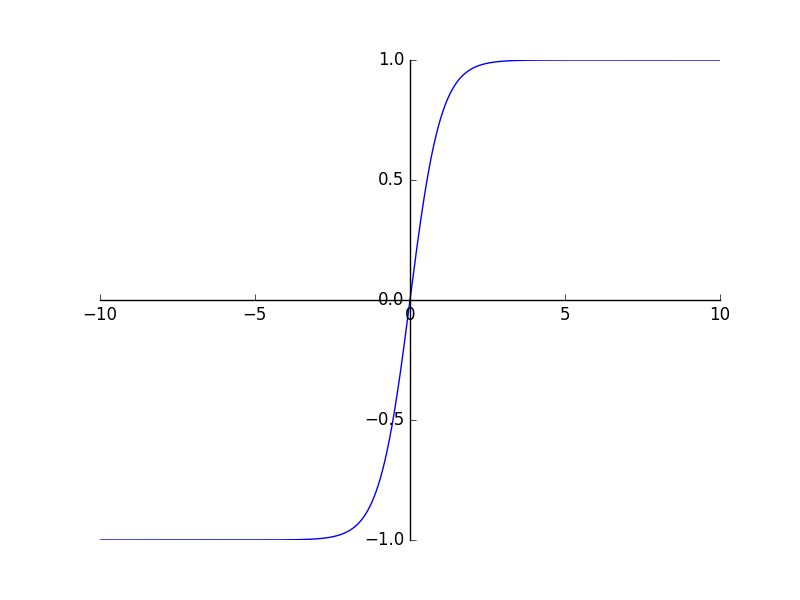
\includegraphics[width = 3in]{img/tanh_activation}}
	\subfigure[$\operatorname{sigmoid}(x) = \frac{1}{1 + e^{-x}}$]{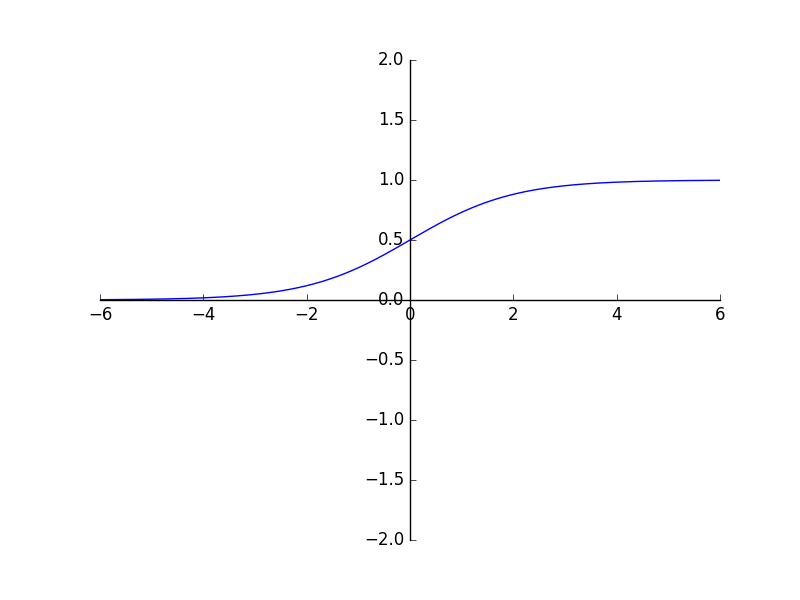
\includegraphics[width = 3in]{img/sigmoid_activation}}
	\subfigure[$\operatorname{relu}(x) = \max\{0,x\}$]{\includegraphics[width = 3in]{img/relu_activation}}
	\subfigure[$\operatorname{binarystep}(x) = \left\{\begin{array}{lr}0 & \text{for }x < 0\\1 & \text{for }x \geq 0\end{array}\right\}$]{\includegraphics[width = 3in]{img/binary_step_activation}}
	\caption{Plots of several commonly used activation functions for neurons in NNs.}
	\label{fundamentals:figures:activation_functions}
\end{figure}

\paragraph{Layer}\label{basic:neural_network:layer} With the neurons introduced one paragraph earlier, we can now start to build the layers of a NN. Each layer consists of multiple neurons stacked on top of each other, as seen in figure \ref{fundamentals:figures:neural_network}. These layers are then arranged in a sequential manner to form a full NN. Each NN usually has at least three of these layers: The first one is called the \emph{input layer}, the second the \emph{hidden layer} and the most right one is the \emph{output layer}.

\begin{figure}[h]
	\centering
	\includegraphics[width=10cm]{img/basic_neural_network}
	\caption{Simplified visualization of a NN with one input, hidden and output layer.}
	\label{fundamentals:figures:neural_network}
\end{figure}

The input data $\mathbf{x} = (x_1, x_2, \dots, x_n)$ is enters the NN through the input layer. At this stage, the bias $x_0$ value is usually set to $1$ again. Most of the time, there is only one bias value and weight for all neurons in a layer of an NN. The input values in $\mathbf{x}$ are then forwarded to the neurons of the (first) hidden layer which then compute their activations $o_{ln}$, where $l$ signifies the layer and $n$ shows the position of the neuron in that layer respectively. The resulting activation values are then passed to the output layer, where the embodied neurons compute their activation values $o_{21}, o_{22}, \dots, o_{2n}$. The input values of a single neuron in the output layer are usually the activation values of all neurons in the preceding layer. Such a layer is also called \emph{fully-connected}, as every neuron uses all values from the preceding layer. The output of the NN is then the set of activation values $o_{31}, o_{32}, \dots, o_{3m}$ in the output layer, where $m$ signifies the number of neurons in the output layer.

This procedure of doing one forward-pass through the NN is called \emph{forward propagation}. Our example only consists of one hidden layer, but one can also imagine NNs with multiple hidden layers; such NNs are then called \emph{deep neural networks}. The number of layers and neurons in each of them is strongly dependent on the nature of the problem it is applied to.

\paragraph{Backpropagation with gradient-descent} As in almost all models in the area of machine learning, a NN learns by optimizing a \emph{loss function} $L$, also sometimes called error function. Every function which can be used to quantify the predictive error of a NN can be used as a loss function. As examples, one could mention the \emph{mean squared deviation} $\operatorname{msd}(y_{true}, y_{pred}) = \frac{1}{n}\sum_{i=0}^{n} (y_{pred} - y_{true})^2$ or the one used for the model of this thesis, the \emph{categorical cross-entropy} function $H(p,q) = -\sum{x} p(x)\operatorname{log}(q(x))$. The optimization of this loss function is almost always done via a method called \emph{backpropagation} in conjunction with the \emph{gradient-descent} algorithm. The optimization is then done as follows:

\begin{enumerate}
	\item Do the forward propagation with the given input values $\mathbf{x} = (x_0, x_1, \dots, x_n)$ as described above.
	\item Use the predicted and expected values in combination with the defined loss function to quanitfy the predictive error of the NN.
	\item The predictive error is now backpropagated through the NN via the gradient-descent algorithm. The weights of all inputs for each neuron are then adapted with respect to their influence on the exhibited predictive error.
\end{enumerate}

The influence of each weight on the predictive error is determined by computing the partial derivate of the loss function $L$ with respect to the respective weights, as seen in equation \ref{fundamentals:equation:gradient_descent}. After computing the partial derivation, the weights are updated accordingly. This is done by multiplying the computed derivation value by the learning rate $\eta$ and subtracting the resulting value from the current value of the weight. The learning rate defines, how strong a single run of gradient-descent alters each weight in the network.

The new value for the weight $i$ in layer $l$, with given learning rate $\eta$ and loss function $L$, is then computed as follows:

\begin{equation}
\label{fundamentals:equation:gradient_descent}
w_{li} \coloneqq w_{li} - \eta \frac{\delta E(\mathbf{w})}{\delta w_{li}}
\end{equation}

In practice, this computation is done in a vectorized manner to speed up the computation significantly. Here we use the gradient (hence the name) of the loss function with respect to all weights $\mathbf{w}$:

\begin{equation}
\mathbf{w} \coloneqq \mathbf{w} - \eta(\nabla_{\mathbf{w}}E(\mathbf{w}))
\end{equation}

One of the big drawbacks of gradient-descent is, that its success is highly dependent on the chosen learning rate $\eta$. When the learning rate is chosen too large, the algorithm might miss the optimium or the value of the loss function even diverges; if the learning rate is too small on the other hand, it might take a really long time until the final optimum is found. We've visualized this problem in figure \ref{fundamentals:figures:learning_rates}, where the development of an arbitrary loss function with different learning rates is plotted over time.

To mitigate this issue, we've chosen to use \emph{AdaGrad} \cite{Duchi:2011} for the model of this thesis, which is an advancement to vanilla gradient-descent. It solves the problem of manually setting a learning rate partially by incorporating blabalbal!!!

\begin{figure}[h]
	\centering
	\includegraphics[width=6cm]{img/learning_rates_comparison}
	\caption{Visualization of the development of a loss function when using different learning rates.\protect\footnotemark}
	\label{fundamentals:figures:learning_rates}
\end{figure}
\footnotetext{http://cs231n.github.io/assets/nn3/learningrates.jpeg}
\chapter{Additional Charts}
\blindtext
\chapter{Using the Software System}
\label{appendix:software_usage}
The following chapter gives a tutorial on how to use the software system (see Chapter~\ref{software_system}) implemented to conduct the experiments in this thesis.

\section{Download}
The code of the software system can be downloaded by using \texttt{git}\footnote{https://git-scm.com/}. The repository is located on the publicly accessible GitHub website\footnote{https://github.ch/vongrdir/BA-ML-17}. However, the visibility of the repository is set to private. To gain access, please send an e-mail with the request and the username of your GitHub account to either \texttt{vongrdir@students.zhaw.ch} or \texttt{weilemar@students.zhaw.ch}.

\section{Requirements}
To use the software and all the related scripts, the following software packages must be installed:

\begin{itemize}[noitemsep]
	\item \texttt{python} in the version 3.5.2\footnote{https://www.python.org/}
	\item If a GPU is used:
	\begin{itemize}[noitemsep]
		\item Nvidia GPU driver\footnote{http://www.nvidia.de/Download/index.aspx} for the respective GPU.
		\item Nvidia \texttt{cuda} 8 toolkit\footnote{https://developer.nvidia.com/cuda-toolkit}.
	\end{itemize}
\end{itemize}

The experiments and script can also be conducted without a GPU and solely on the CPU. However, this leads to higher runtime in several parts of the system, mainly when training models. In addition to the mentioned software packages the \texttt{python} libraries listed in Chapter~\ref{software_system:software_packages} must be installed.

The libraries can be installed via the \texttt{python} package manager \texttt{pip}\footnote{https://packaging.python.org/installing/}. It is recommended to us the exact versions of the mentioned software packages and \texttt{python} libraries to avoid any compatibility issues. However, it might certainly be possible that the software system runs find with newer version without any problems.

\clearpage
\section{Structure of the Repository}
In the following table, we explain the structure of the repository and the contents of the main directories.

\begin{table}[H]
	\centering
	\begin{tabularx}{\textwidth}{lX}
		\toprule
		Name of Directory & Description\\ \midrule
		\texttt{configs/} & In this directory, all the JSON configurations for all experiments are stored.\\
		\texttt{report/} & All documents related to the thesis are stored in this directory.\\
		\texttt{misc/} & Directory for storing miscellaneous files.\\
		\texttt{results/} & The results of all the run experiments are stored in this directory. The results themselves are stored in a directory named after the \texttt{WHAT} of the experiment. In total, the model, all collected metrics and the configuration of experiments are stored in this directories.\\
		\texttt{scripts/} & The scripts used in this thesis are stored in this directory (see Chapter~\ref{software_usage:using_scripts}).\\
		\texttt{source/} & The whole source code of the software system itself is located in this directory including all the components necessary to implement the system described in the Chapter~\ref{sofware_system}.\\
		\bottomrule
	\end{tabularx}
	\caption{Remarks regarding the structure of the repository.}
\end{table}

\clearpage
\section{Using the Scripts}
\label{software_usage:using_scripts}
In the following section, we are going to introduce the most important scripts necessary to use the software system for running experiments. The scripts themselves are located in the directory \texttt{scripts/}.

\begin{table}[H]
	\centering
	\ra{1.3}
	\begin{adjustbox}{max width=\textwidth}
		\begin{tabular}{lp{8cm}p{8cm}}
			\toprule
			Name & Description\\ \midrule
			\texttt{analyse{\_}ngram{\_}from{\_}corpus.py} & With this script, it is possible to analyse a corpus regarding its bigrams. This script was used to generate the n-grams in Chapter~\ref{chapter:data:ngram} and~\ref{results:development_language_model}.\\
			\texttt{analyze{\_}timestamp{\_}problematic{\_}opensubtitles.py} & With this script, the time-lag analysis between utterances in the OpenSubtitles corpus can be done (see Chapter~\ref{data:opensubtitles:time_lag_analysis}).\\
			\texttt{analyze{\_}word{\_}coverage.py} & This script allows to analyse the word coverage of a corpus with regard to a given vocabulary (see Chapter~\ref{data:word_coverage}).\\
			\texttt{split{\_}corpus.py} & This script allows to split a given corpus into a training, test and validation set by proportions. The split itself is done randomly (see Chapter~\ref{data:split_corpus}).\\
			\texttt{evaluate{\_}trained{\_}model.py} & This script allows to evaluate a trained model on a certain dataset and stores the resulting metrics of this evaluation.\\
			\texttt{generate{\_}s2v{\_}sequence{\_}embeddings.py} & This script allows for generating Sent2Vec embeddings for the given list of sequence samples. These are then used in Chapter~\ref{results:performance_on_test_datasets} for the similarity analysis.\\
			\texttt{get{\_}internal{\_}embeddings{\_}from{\_}samples.py} & This script allows to generate thought vectors for a list of given sample texts. They are used in the analysis in Chapter~\ref{results:thought_vector_clustering}.\\
			\texttt{preprocess{\_}opensbutitles{\_}data.py} & This script is responsible for preprocessing the raw OpenSubtitles corpus as described in Chapter~\ref{data:preprocessing}.\\
			\texttt{preprocess{\_}reddit{\_}corpus.py} & This script is responsible for preprocessing the raw Reddit corpus and building the tree which is the finally converted into the datasets as described in Chapter~\ref{data:preprocessing}.\\
			\texttt{talk{\_}to{\_}model.py} & This script provides a possibility to talk to trained models through the terminal. The functionality is basically the same as in the web frontend (see Chapter~\ref{sofware_usage:web_frontend}).\\
			\bottomrule
		\end{tabular}
	\end{adjustbox}
	\caption{Descriptions of the most important scripts to use the software system.}
\end{table}

There are much more scripts than the ones described above (e.g. for plotting, creation of vocabularies). Not all of them are necessary to conduct experiments, which is why only explain the most important.

In the following table there are exemplary calls for all scripts listed above:

\begin{table}[H]
	\centering
	\ra{1.3}
	\begin{adjustbox}{max width=\textwidth}
		\begin{tabular}{lp{20cm}}
			\toprule
			Name & Exemplary Call\\ \midrule
			\texttt{analyse{\_}ngram.py{\_}from{\_}corpus.py} & python scripts/analyse{\_}ngram.py{\_}from{\_}corpus.py data/opensubtitles/opensubtitles\_raw.txt 2 results/opensubtitles/bigram\_analysis.csv results/opensubtitles/bigram\_analysis\_words.csv\\
			\texttt{analyze{\_}timestamp{\_}problematic{\_}opensubtitles.py} & python scripts/analyze{\_}timestamp{\_}problematic{\_}opensubtitles.py data/OpenSubtitles2016 analysis\_timestamps\_opensubtitles.json\\
			\texttt{analyze{\_}word{\_}coverage.py} & python scripts/analyze{\_}word{\_}coverage.py data/reddit/reddit\_corpus.txt word\_coverage\_reddit\_new.json data/reddit/vocab\_100k.pickle,data/reddit/vocab\_50k.pickle\\
			\texttt{split{\_}corpus.py} & Tpython scripts/split{\_}corpus.py data/reddit/reddit\_corpus\_preprocessed.txt 80,10,10 data/reddit/reddit\_train.txt data/reddit/reddit\_valid.txt data/reddit/reddit\_test.txt\\
			\texttt{evaluate{\_}trained{\_}model.py} & python scripts/evaluate{\_}trained{\_}model.py results/reddit/model-100000.chkp data/reddit/reddit\_train.txt results/reddit/test\_metrics.json results/reddit/test\_predictions.csv 250000\\
			\texttt{generate{\_}s2v{\_}sequence{\_}embeddings.py} & python scripts/generate{\_}s2v{\_}sequence{\_}embeddings.py misc/fasttext misc/sent2vec\_wiki\_bigrams 700 2 results/reddit/test\_predictions.csv results/reddit/test\_s2v\_generated\_wiki\_bigrams.h5\\
			\texttt{get{\_}internal{\_}embeddings{\_}from{\_}samples.py} & python scripts/get{\_}internal{\_}embeddings{\_}from{\_}samples.py samples.txt results/reddit/model-100000.chkp results/reddit/samples\_embeddings.h5\\
			\texttt{preprocess{\_}opensubtitles{\_}data.py} & python scripts/preprocess\_opensubtitles\_data.py data/opensubtitles/raw-xml-files/ data/opensubtitles/opensubtitles\_raw.txt\\
			\texttt{preprocess{\_}reddit{\_}corpus.py} & python script/preprocess\_reddit\_corpus data/reddit/full\_corpus/ 2014,2015 movies\\
			\texttt{talk{\_}to{\_}model.py} & python scripts/talk\_to\_model.py\\
			\bottomrule
		\end{tabular}
	\end{adjustbox}
	\caption{Exemplary calls for the most important scripts to use the software system.}
\end{table}

\clearpage

\section{Running Experiments}
\label{software_usage:running_experiments}
To run experiments, one has to write a configuration file in the JSON format. All of them reside in the directory \texttt{configs/}. In the following table, all important configuration parameters are explained:

\begin{table}[H]
	\centering
	\ra{1.3}
	\begin{adjustbox}{max width=\textwidth, max height=\textheight}
		\begin{tabular}{llp{10cm}}
			\toprule
			Name & Default Value & Description\\ \midrule
			\texttt{device} & \texttt{/gpu:0} & Defines the device on which the computations are run.\\
			\texttt{train} & \texttt{true} & Defines whether a training should be run or not. Is set to \texttt{false} in case inference is run.\\
			\texttt{git\_rev} & \texttt{null} & This parameter stores the SHA1 of the latest \texttt{git} revision when an experiment was started.\\
			\texttt{model\_path} & \texttt{null} & This parameter signifies if an already trained model should be loaded before starting the training or inference.\\
			\texttt{training\_data} & \texttt{null} & Defines which dataset should be used for training the model while training.\\
			\texttt{validation\_data} & \texttt{null} & Defines which dataset should be used for validating the model while training.\\
			\texttt{reverse\_input} & \texttt{false} & Defines whether the input sequence should be fed to the model in reverse if set to \texttt{true}.\\
			\texttt{use\_last\_output\_as\_input} & \texttt{false} & Defines whether the output of the last sample should be used as the input for the next sample.\\
			\texttt{start\_training\_from\_beginning} & \texttt{false} & Defines whether the training should start from the first sample of the training dataset or not. If it is set to \texttt{true}, the training will start with the first sample the model has not already seen in previous trainings, as indicated by internal variables of the model saved when storing the model.\\
			\texttt{show{\_}predictions\_while\_training} & \texttt{false} & Defines whether the outputs of the model should be printed to the terminal when training.\\
			\texttt{show{\_}predictions\_while\_training\_num} & \texttt{5} & Defines how much predictions should be printed at the end of each epoch when training.\\
			\texttt{vocabulary} & \texttt{null} & Defines which \texttt{pickle} vocabulary should be used for the current model.\\
			\texttt{epoch} & 1 & Defines the number of epochs which should be done in case of training a model.\\
			\texttt{save\_model\_after\_n\_epochs} & \texttt{10} & Defines the interval in which the model is stored based on the number of epochs finished.\\
			\texttt{epochs\_per\_validation} & \texttt{10} & Defines the interval in which the model is validated while training based on the number of epochs finished.\\
			\texttt{batches\_per\_validation} & \texttt{0} & Defines the interval in which the model is validated while training based on the number of epochs finished.\\
			\texttt{batches\_per\_epoch} & \texttt{1000} & Defines how much batches should be processed in one epoch.\\
			\texttt{batch{\_}size} & \texttt{1} & Defines how much samples should be put in one batch.\\
			\bottomrule
		\end{tabular}
	\end{adjustbox}
	\caption{Explanation of the important configuration parameters of the software system (part 1).}
\end{table}

\clearpage

\begin{table}[H]
	\centering
	\ra{1.3}
	\begin{adjustbox}{max width=\textwidth, max height=\textheight}
		\begin{tabular}{llp{10cm}}
		\toprule
		Name & Default Value & Description\\ \midrule
		\texttt{max{\_}input\_length} & \texttt{50} & Defines the maximum number of words to consider from the input sequence.\\
		\texttt{max{\_}output\_length} & \texttt{50} & Defines the maximum number of words the decoder can generate before the decoding stops.\\
		\texttt{num{\_}encoder\_layers} & \texttt{1} & Partially defines the number of layers to use for the encoder and decoder. This number is added to \texttt{num{\_}decoder\_layers} to get the full number of layers for the encoder and decoder.\\
		\texttt{num{\_}decoder\_layers} & \texttt{1} & Partially defines the number of layers to use for the encoder and decoder. This number is added to \texttt{num{\_}encoder\_layers} to get the full number of layers for the encoder and decoder.\\
		\texttt{num{\_}hidden\_units} & \texttt{1024} & Defines the size of the hidden state used in the encoder and decoder cell.\\
		\texttt{cell{\_}type} & \texttt{LSTM} & Defines which kind of RNN cell is used for the model. Can be either \texttt{LSTM}, \texttt{GRU} or \texttt{RNN}.\\
		\texttt{sampled{\_}softmax\_number\_of\_samples} & \texttt{512} & Defines the number of words sampled when using the sampled softmax loss function. Is disabled in case the number of words is smaller than the provided number or if the parameter is set to 0.\\
		\texttt{hidden\_state\_reduction\_size} & \texttt{null} & Defines the dimensionality the hidden state of the decoder cell should be projected down to before it is fed to the softmax layer at the end.\\
		\texttt{max\_random\_embeddings\_size} & \texttt{512} & Defines the dimensionality of the word embeddings used within the model.\\
		\texttt{use\_beam\_search} & \texttt{false} & Defines whether the beam search decoder should be used instead of the greedy decoder.\\
		\texttt{beam\_size} & \texttt{10} & The number of beams which should be considered when using the beam search decoder.\\
		\texttt{beam\_search\_only\_best} & \texttt{true} & Defines that the output of the beam search decoder should only be the one resulting from the best beam if set to \texttt{true}, or the results from all beams otherwise.\\
		\texttt{buckets} & \texttt{[[50, 50]]} & Defines the buckets which are used when using the model. We only used one bucket, but it is certainly possible to use multiple of them. The range of available buckets has to cover \texttt{max{\_}input\_length} and \texttt{max{\_}output\_length}.\\
		\texttt{dropout\_input\_keep\_prob} & \texttt{1.0} & Defines how much percent of the input to the RNN cells should be kept when using dropout.\\
		\texttt{dropout\_input\_keep\_prob} & \texttt{1.0} & Defines how much percent of the output of the RNN cells should be kept when using dropout.\\
		\bottomrule
		\end{tabular}
	\end{adjustbox}
	\caption{Explanation of the important configuration parameters of the software system (part 2).}
\end{table}

One peculiarity can be seen from the names of the configuration parameters: Some of them contain the word \emph{epoch}, but not necessarily refer to the definition of epoch found in the glossary. This is related to the way training works with TensorFlow, as it does use the term epoch differently. Instead of referring to one full iteration over the training corpus, it refers to a fixed number of batches being processed, because TensorFlow itself has no notion of epoch but rather uses the term \emph{step}. A fixed number of steps is then called an epoch.

The descriptions above are neither complete nor concluding. We recommend consult the source code for the exact behavior of the additional parameters. Also, there are more model related parameters which are only applicable to the models stored in the source code file \texttt{other\_models.py}, where implemented, but now unused models reside.

\clearpage

An example configuration can look as follows:

\begin{figure}[thp]
	\centering
	\begin{tabular}{c}  % the tabular makes the listing as small as possible and centers it
		\begin{lstlisting}[style=json]
		{
			"epochs": 150000,
			"batches_per_epoch": 100,
			"batches_per_validation": 2500,
			"epochs_per_validation": 50,
			"save_model_after_n_epochs": 100,
			"batch_size": 64,
			"cell_type": "LSTM",
			"num_hidden_units": 2048,
			"hidden_state_reduction_size": 1024,
			"num_encoder_layers": 1,
			"num_decoder_layers": 1,
			"training_data": "data/reddit_train.txt",
			"validation_data": "data/reddit_valid.txt",
			"vocabulary": "data/reddit/vocab_50k.pickle",
			"max_random_embeddings_size": 1024,
			"max_input_length": 30,
			"max_output_length": 30,
			"reverse_input": false,
			"show_predictions_while_training": true,
			"buckets": [[30, 30]],
			"sampled_softmax_number_of_samples": 512,
			"word_tokenizer": "none",
			"use_last_output_as_input": false,
			"start_training_from_beginning": false
		}
		\end{lstlisting}
	\end{tabular}
	\label{software_usage:config_json_example}
	\caption{Example JSON configuration for the Reddit experiment.}
\end{figure}

To start experiments, one has to invoke the \texttt{run.sh} script at the root of the repository with the configuration of the experiment desired to run.

\texttt{\$ ./run.sh configs/config-1.json}

The results are then stored in a directory in \texttt{results/} within a subdirectory named after the name of the configuration file supplied to \texttt{run.sh}.

\section{Web Frontend}
\label{sofware_usage:web_frontend}
We implemented a simple web frontend for communicating with already trained models. It is implemented by using \texttt{flask}, \texttt{jQuery}\footnote{https://jquery.com/} and the \texttt{bootstrap}\footnote{http://getbootstrap.com/} frontend framework. To us the frontend, one has to start it using the following command from the root of the project:

\texttt{\$ python scripts/web/app.py}

This will start the web frontend running on \texttt{localhost} and using the port 9001. After it has been started, one has to select the model it would like to load from the models in the dropdown at the top. All models found in the \texttt{results/} directory (which can be loaded) are listed there. After the selection, a session has to be started by clicking on the \emph{Start} button. This might take a moment, as the loading of the model is a costly process. After the model has been loaded (as indicated by ...), one can start to communicate with it by sending text. Keep in mind, that the kind of output of the model (e.g. beam-search or greedy) directly depends on the configuration stored in the directory where the loaded model is located. This means, if one wants to see for example the output of all beams (in case of beam-search), one has to change the configuration value of the key \texttt{beam\_search\_only\_best} to \texttt{false} there. For a comprehensive list of all configuration values and their meaning, please see Chapter~\ref{software_usage:running_experiments} or the source code itself.
\\
\begin{figure}[H]
	\centering
	\includegraphics[width=10cm]{img/web_frontend_inference}
	\caption{Frontend showing the output when sending the sequence ``1 2 3 4 5'' to a model trained on the copy task (see chapter \ref{software_sytem:model_validation_checks}).}
\end{figure}

One last remark: Currently, there is still a bug when the user tries to end a running session and start a new one. The work around is to simply restart the entire web application.

\end{appendices}
% Glossar entries

\newglossaryentry{cell}
{
	name={Cell},
	description={Any instance of any kind of RNN layer is called a cell}
}

\newglossaryentry{corpus}
{
	name={Corpus},
	description={Refers to the raw data used to build the datasets}
}

\newglossaryentry{dataset}
{
	name={Dataset},
	description={Refers to the dataset resulting from the preprocessing of the raw corpus}
}

\newglossaryentry{epoch}
{
  name={Epoch},
  description={One iteration through all of the training data is called an epoch}
}

\newglossaryentry{encoder}
{
	name={Encoder},
	description={Part of seq2seq models responsible for processing the input sequence}
}

\newglossaryentry{decoder}
{
	name={Decoder},
	description={Part of seq2seq models responsible for generating the output sequence}
}

\newglossaryentry{neuron}
{
  name={Neuron},
  description={Basic building blocks of NN. Models a mathematical function}
}

\newglossaryentry{layer}
{
  name={Layer},
  description={Collection of multiple neurons. An NN usually consists of several of these layers}
}

% Acronyms
\newacronym{CPU}{CPU}{Central Processing Unit}
\newacronym{GPU}{GPU}{Graphical Processing Unit}
\newacronym{NN}{NN}{Neural Network}
\newacronym{RNN}{RNN}{Recurrent Neural Network}
\newacronym{LSTM}{LSTM}{Long Short-Term Memory Network}
\newacronym{Seq2Seq}{Seq2Seq}{Sequence-To-Sequence}


\glsaddall
\printglossary[type=\acronymtype,title=Glossary]
\listoftables
\listoffigures
\printbibliography[heading=bibintoc]


\end{document}
